%% Template for Master thesis
%% ===========================
%%
%% You need at least KomaScript v3.0.0,
%% e.g. available in Texlive 2009
\documentclass  [
  paper    = a4,
  BCOR     = 10mm,
  twoside,
  fontsize = 12pt,
  fleqn,
  toc      = bibnumbered,
  toc      = listofnumbered,
  numbers  = noendperiod,
  headings = normal,
  listof   = leveldown,
  version  = 3.03
]                                       {scrreprt}

% used pagages
%\usepackage[margin=10pt,font=small,labelfont=bf,labelsep=endash]{caption}
\usepackage     [utf8]          {inputenc}
\usepackage     [T1]            {fontenc}
\usepackage                     {color}
\usepackage                     {amsmath}
\usepackage                     {graphicx}
\usepackage     [english]       {babel}
\usepackage     [round]         {natbib}

\usepackage                     {hyperref}
\usepackage						{cleveref}
\usepackage						{subfigure}
\usepackage						{multirow}
\usepackage						{booktabs} % Allows the use of \toprule, \midrule and \bottomrule in tables
\usepackage						{multicol} % Required for creating multiple columns in slides
\usepackage		[version=4]		{mhchem}
%\usepackage{cvpr}
%\usepackage{times}
\usepackage{epsfig}
\usepackage{amssymb}
% links
\definecolor{darkblue}{rgb}{0.0,0.0,0.4}
\definecolor{darkgreen}{rgb}{0.0,0.4,0.0}
\hypersetup{
    colorlinks,
    linkcolor=black,
    citecolor=darkgreen,
    urlcolor=darkblue
}
%\renewcommand{\partname}{}
%\renewcommand{\thepart}{}

\begin{document}
  %% title pages similar to providet template instead of maketitle
  %% this will generate title pages similar to the template provided
%% by the Department of Physics and Astronomy Heidelberg
%%
%% More information:
%% http://www.physik.uni-heidelberg.de/aktuelles/studium/
%% (PDF link: ...studium/download/145/Vorlage_Diplomarbeit_Formular.pdf)

%% Titleintro
\thispagestyle{empty}
\begin{center}
  \renewcommand{\baselinestretch}{2.00}
  \Large\sffamily
  Department of Physics and Astronomy\\
  \large University of Heidelberg
  \par\vfill\normalfont
  Master thesis\\
  in Physics\\
  submitted by\\
  Elsa  Wilken\\
  born in Hamburg\\
  2018
\end{center}
\newpage

%% Titlepage
\thispagestyle{empty}
\begin{center}
  \renewcommand{\baselinestretch}{2.00}
  \Large\bfseries\sffamily
    Retrieval Advances of BrO/\ce{SO2}              \\
    Molar Ratios from NOVAC\\
  \par
  \vfill
  \large\normalfont
  This Master thesis has been carried out by Elsa Wilken\\
  at the\\
  Institute for Environmental Physics, University of Heidelberg, Germany\\
  under the supervision of\\
  Prof. Ulrich Platt,\\
  Dr. Nicole Bobrowski,\\
  Florian Dinger
  %% additionally insert second supervisor here if carrying out an
  %% external diploma thesis. Reduce vspace in L. 44 accordingly.
\end{center}\par
\vspace{5\baselineskip}

% reset baselinestretch
\renewcommand{\baselinestretch}{1.00}\normalsize % or english title page
  %% Abstract page
%% =============
%%
%% Content of abstract pages has been put into seperate pages to simplify
%% word counting. Use e.g. the unix command
%%   wc abstract-ger.tex
%% or
%%   wc abstract-eng.tex
%% to get the number of words contained in these files.
\thispagestyle{empty}
\begin{center}
  \begin{minipage}[c][0.48\textheight][b]{0.9\textwidth}
    \small
    \textbf{Optimierte Bestimmung des molaren BrO/\ce{SO2} Verhältnisses aus NOVAC Daten
    }\par
    \vspace{\baselineskip}
    %% Latex markup und Zitate funktionieren auch hier


Die Messung der absoluten Menge und von Konzentrationsverhältnissen vulkanischer Gas Emissionen geben Einsicht in magmatische Prozesse. Das Network for Observation of Volcanic and Atmospheric Change (NOVAC) besteht aus einem System von automatisierten UV-Spektrometern, welche die Gas Emissionen der Vulkane aufzeichnen. Die Emission von BrO und \ce{SO2} kann mithilfe von Differenzieller optischer Absorptionsspektroskopie (DOAS) aus den aufgenommen Spekren bestimmt werden wobei die optische Absorption in der Fahne mit einem Reference Spectrum verglichen wird. Dies setzt voraus, dass das Reference Spectrum frei von Vulkanische Gasen ist. Typischerweise wird das Reference Spectrum für einen Scan bei einem Elevationswinkel aufgenommen welcher welcher so gewählt wird dass das Instrument nicht in die Fahne schaut. Es hat sich jedoch gezeigt, dass auch diese Spektren noch durch Vulkanische Emissionen verunreinigt sein können. Als alternative Referenzspektren könnten 1) ein theoretisches Solar Atlas Spektrum oder 2) ein nicht verunreinigtes Referenz Spektrum des selben Messgeräts dienen. Option 1) hat den Nachteil einer verringerten Messgenauigkeit, da Instrumenteneffekte hier modelliert werden müssen und ist daher nur für das typischerweise in hoher Konzentration vorkommende \ce{SO2} anwendbar. Option 2) setzt voraus, dass das Referenzspektrum unter ähnlichen Wetter- und Strahlungsbedingungen aufgenommen wurde. Wir verwenden die erste Methode um (\ce{SO2}) Kontaminierung zu identifizieren und greifen für die Bestimmung der Gas Konzentration auf die zweite Methode zurück um eine hohe Qualität der Messung sicher zu stellen. Im Folgenden stellen wir unsere Methode für NOVAC Daten von den Vulkanen Tungurahua und Nevado Del Ruiz vor.
  \end{minipage}\par
  \vfill
  \begin{minipage}[c][0.48\textheight][b]{0.9\textwidth}
    \small
    \textbf{Retrieval advances of BrO/\ce{SO2} molar ratios from NOVAC
    }\par
    \vspace{\baselineskip}
    %% Latex markup and citations may be used here

%Measurements of magnitude and composition of volcanic gas emissions allow insights in magmatic processes. Within the Network for Observation of Volcanic and Atmospheric Change(NOVAC) automatically scanning UV-spectrometers are monitoring gas emission at volcanoes. The emissions of BrO and \ce{SO2} can be retrieved from the recorded spectra by applying Differential Optical Absorption Spectroscopy(DOAS) and comparing the optical absorption of the volcanic plume to the background. Therefore, the background spectrum must not be affected by volcanic influence. Conventionally, the background spectrum is taken from the same scan but from an elevation angle which has been identified to be outside of the volcanic plume. However, experience shows those background spectra can still be contaminated by volcanic gases.  Alternatively, background spectra can be derived from 1) a theoretical solar atlas spectrum or 2) a volcanic-gas-free background spectrum recorded by the same instrument at another time. 1) comes with a drawback of reduced precision, as the instrumental effects have to be modeled and added to the retrieval. For 2), the alternative background spectrum should be recorded at similar conditions with respect to meteorology and radiation. We use the first option to check for contamination and the second to evaluate the spectra to maintain a good fit quality. We present our approach and its results when applied on NOVAC data from Tungurahua and Nevado del Ruiz.

Measurements of magnitude and composition of volcanic gas emissions allow insights into magmatic processes. In this thesis, the concentration ratio of BrO and \ce{SO2} is analyzed. The measurements are performed with scanning UV-spectrometers provided by the "Network for Observation of Volcanic and Atmospheric Change (NOVAC)".
The concentrations are then retrieved by applying Differential Optical Absorption Spectroscopy (DOAS).
For this purpose, especially weak absorbers like BrO require a gas-free reference spectrum to eliminate the Fraunhofer structures.
However, with the conventional evaluation approach, it is still possible that the chosen same-time-reference spectra are contaminated. Alternative reference spectra could be (1) a theoretical solar atlas spectrum or (2) a temporal shifted uncontaminated reference spectrum which is recorded by the same instrument. (1) comes with the drawback of a decreased measurement precision, as instrumental effects must be modeled, while (2) only works with a reference that is recorded under similar conditions as the measurement spectrum. In this work, a new approach is presented which uses (1) for the identification of (\ce{SO2}) contamination and (2) for the actual measurement of the gas concentration. The novel approach sidesteps the systematic underestimation of the concentration and increases the amount of reliable data by approximately 30\%. Moreover, we are able to prove the occurrence of BrO contamination.
  \end{minipage}
\end{center}


  \tableofcontents
  %% Put your contents here
	\chapter{Introduction}	
	
%% Introduction page
%% =============
%%
Volcanic activities on Earth have  always shaped the earth surface and influenced atmospheric processes. Volcanoes are often particularly recognized by their dramatic consequences of a major volcanic eruption. But volcanoes influence our lives in more than this way. Volcanic gases can effect the weather (timescales of days to weeks) or the climate (timescales of months to years) \cite{schmidt2015volcanismarticle}.
Examples are the lake eruption in Iceland (1783-1784) followed by a very hot summer and a cold winter in central Europa \cite{thordarson2003atmospheric} and the Tambora eruption, indonesia in 1815 which caused the "year without summer" in 1816.\\
%
\newline
%
Considering the plate tectonics of earth  most volcanoes are caused by diverging or converging of the continental plates and therefore located at the margins of the continental plates.
Another possibility for occurrence of volcanoes is the the interior of continental or oceanic shelves. \cite{schmincke2000vulkanismus}\\
The most abundant volatile species released during a volcanic eruption are water vapour (H$_2$O; relative amount of the plume: 50\%-90\%) and carbon dioxide (CO$_2$; relative amount of the plume: 1\%-40\%) \cite{platt2015quantification}. But the short effects of those two gases are rather low since there effect on atmospheric composition is negligibly due to the high abundance of atmospheric H$_2$O and CO$_2$. But on timescales of the age of the earth the volcanic emission of H$_2$O and CO$_2$ are the source of our current atmosphere. \cite{schmidt2015volcanism}\\ 
A typically volcanic plume consists of many different gases alongside H$_2$O and CO$_2$  sulfur dioxide (SO$_2$) contributes with 1\%-25\% to the plume, hydrogen sulfide (H$_2$S) with 1\%-10\% and hydrogen chloride with (HCl) 1\%-10\%. Furthermore there are trace gases for example carbon disulfide (CS$_2$), carbon sulfide (COS) carbon monoxide (CO) hydrogen fluoride (HF) and hydrogen bromide (HBr) \cite{platt2015quantification}\\
%
A decrease of stratospheric ozone (O$_3$) has been observed after the eruption of  El Chickon in 1982 and the eruption of mount Pinatubo 1991. A depletion stratospheric O$_3$ results in ozone holes. The depletion comes from volcanic aerosols which serve anthropogenic chlorine/bromine into more reactive forms \cite{solomon1998ozone}. 
%
Volcanic gases can alter the radiative balance of the earth in timescales relevant for climate change due to scatter and absorption of solar radiation \cite{schmidt2015volcanism}.\\
%
The gas composition of the volcano plume change with activity and could be a indication for the processes inside the earth.\\ 
%
In this work we are particularly interested in the ratio of BrO and SO$_2$. The halogen sulfur ratio is a proxy for volcanic processes. Therefore we make the assumption
that the ratio of BrO and SO2 contains informations about its degassing source depth. A change in BrO/SO2 prior to eruption was observed at Etna and Nevado del Ruiz.\\
%
\newline
%
To gain further knowledge about the volcanoes the Network for Observation of Volcanic and Atmospheric Change (NOVAC) was installed. NOVAC is a Network of DOAS Instruments located next to about 30 volcanoes in America, Africa and Europe. At every Volcano there are two to four DOAS Instruments installed, recording record back-scattered solar radiation spectra at different viewing angles.\\
NOVAC is a network which produces a large amount of data and we have the chance to evaluate long time periods which is a unique opportunity to study correlations of the trace gases.\\
Since the conditions at volcanoes are rough, the instruments need to be rather simple to keep the maintenance cheap and to assure a longer lifetime of the instruments. So we need to waive on temperature stabilization even at the expense of the quality of the data.\\
%
\newline
%
One possibility to measure the volcanic trace gases is to use Differential Optical Absorption Spectroscopy \cite{platt2008differential}. DOAS exploit the wavelength dependency of the absorption of light. Here the gas emissions can be retrieved
from the quotient of the absorption signal of the volcanic plume and a
reference region. This will be explained in a further chapter.\\
%
\newline
%
The reference region, is usually treated as free of
volcanic trace gases. If the reference region is for any reason
contaminated by volcanic trace gases, the reference spectrum has to be
replaced by a volcanic-gas-free reference. Alternative spectra could be for example a
theoretical solar atlas spectrum or a volcanic-gas-free reference
spectrum recorded in the temporal proximity(eg. a day before) by the same instrument. 
The first option comes with the drawback of reduced precision, as the
instrumental effects have to be modeled and added to the retrieval. The
reduction in precision is acceptable for the SO2 retrieval, but not suitable
for a BrO retrieval because then most data would be below the detection
limit. For the second option, the alternative reference spectrum should
have been recorded at similar conditions with respect to meteorology and
radiation as well as in the temporal proximity due to instrumental changes
with time and ambient conditions. We combined both options in order to
achieve both, enhanced accuracy but still maximum possible precision of
the SO2 and BrO retrievals. We present an algorithm which finds the
optimal reference spectrum automatically. As first step, a possible SO2
contamination of the standard reference is checked by a comparison with
the theoretical solar atlas. If a contamination is detected, as second step,
the algorithm picks a volcanic-gas-free reference (beforehand
automatically checked for contamination) from another scan.\\
%
\newline
%
In this work we are mainly dealing with data from Tungurahua in Ecuador in the timespan of 01.08.2008 to 30.07.2009. Later on, we will also show the results of Nevado del Ruiz a volcano located in Colombia.\\
    \part{Theoretical background}
\chapter{Volcanism and volcanic chemistry}

\section{Volcanism}
The high thermal energy in the deep interior of the earth is mostly well separated from the earth’s surface by the earth’s crust. A volcano is geological structure that allows magma to reach the earth’s surface. Such a phenomenon can occur in various ways. In the following paragraphs the different types of volcanoes are described.
\paragraph{ Mid-ocean ridge volcanism}
The mid-ocean ridge volcanism can be traced back to tectonic processes of oceanic plates. The spreading of two plates, that are pulled apart, leads to a thinning of the oceanic earth crust. This way solid material from the upper mantel (lower than 100 km) can ascend to depths of approximately 50 km. As the pressure at this depth is much lower, the mantle material starts to melt to basaltic magma that fills the gap between the two plates.
\paragraph{ Continental rift zone volcanism}
Similar to mid-ocean ridge volcanism continental rift zone volcanism results from two continental plate are pulled apart.
\paragraph{ Subduction zone volcanoes}
Subduction zone volcanoes occur if an oceanic plate converges under another plate (oceanic or continental). This way the descending plate penetrate into the lower mantle. At a depth of 80-150 km the water of this plate evaporates and rises and causes the mantle material above to melt. The resulting water-rich magma mainly consists of andesite. Subduction zone volcanoes are known for their violent eruptions caused by the low viscosity magma.
\paragraph{ Hot-spot volcanoes} Hot-spot volcanoes occur on continental or oceanic plates. This type of volcanoes arises from a hot spot at the coremantle boundary inside Earth that leads to a plume in the mantle where solid material can rise. This material melts to basaltic magma at a depth of 100-150 km. Through a futher rise also other types of magma (e.g. rhyolitic, more-viscous magma) can arise.


\section{Volcanic gases and their impact on the climate}
\begin{figure}
	\centering
	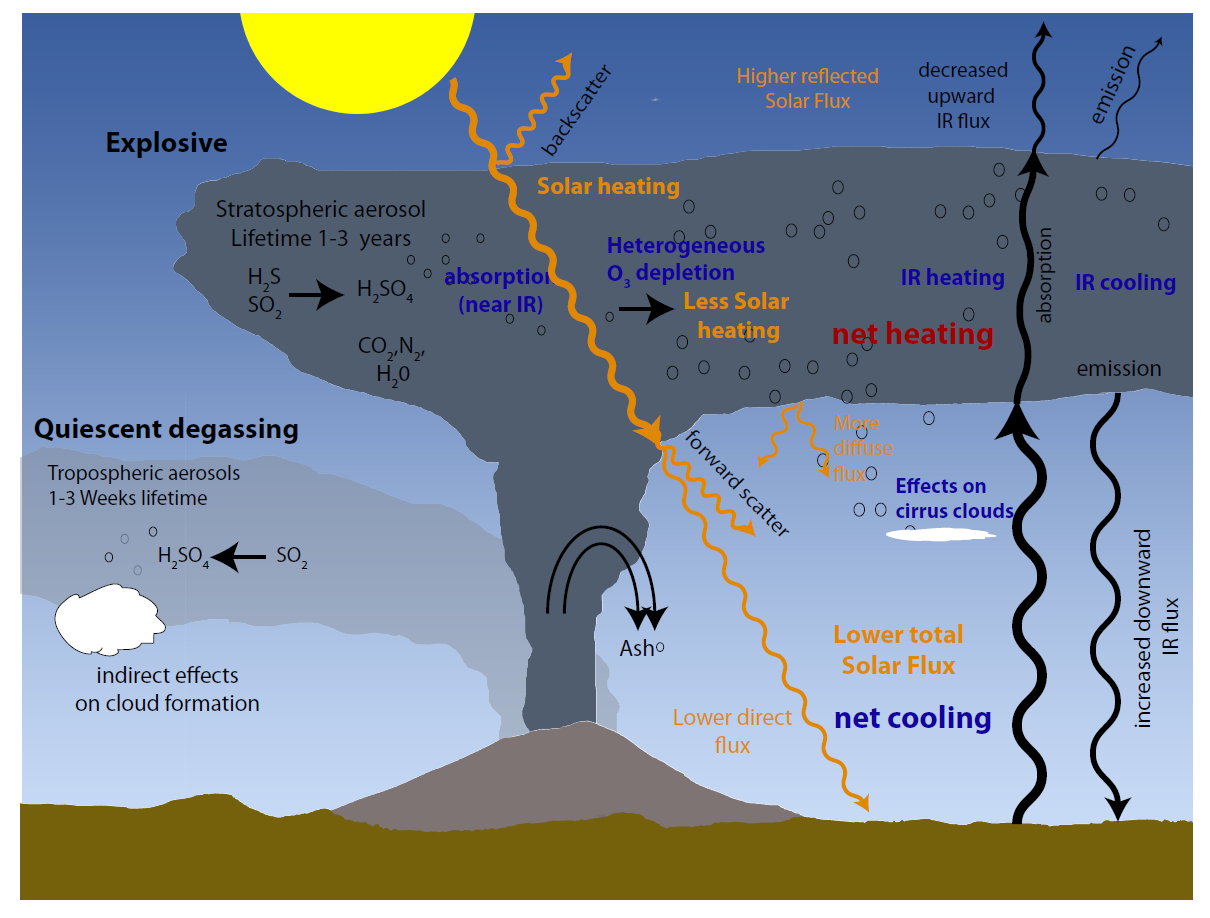
\includegraphics[width=0.8\linewidth]{Bilder/Simon/Bilder_Tung/Climate_Influence}
	\caption{Influence of volcanic eruptions and quiet degassing on earth climate. Redrawn on the basis of \cite{robock2000volcanic}}
	\label{fig:climateinfluence}
\end{figure}
Volcanoes emit various gases (see \cref{tab.volcemissions}) in the atmosphere. This can occur due to volcanic eruptions or due quiet degassing. Gas emitted by quiet degassing remains in the troposphere while eruptions can inject volcanic gases up to the stratosphere \citet{robock2000volcanic}. Due to the larger lifetime in the stratosphere and a larger sensitivity of the stratospheric chemistry to the volcanic gases, these gases have a larger impact on the earth climate as will be discussed for SO2 below.
Volcanic gases have a large impact on the earth climate especially CO2 and \ce{SO2}  or more specific its oxidation product sulfur acid.\\ 
The relevance of  \ce{CO2} for the climate is a subject of many discussions, the share of volcanic  \ce{CO2} is rather low further informations can be found in:...\\\\
Even though the emissions during eruptive episodes are up to one order higher than during quite degassing episodes, \cite{halmer2002annual} estimated that quiescent degassing contributes 40\% of the accumulated SO2 between 1972 to 2000.\\
\cite{halmer2002annual} estimated the mean annual \ce{SO2}  emitted from volcanoes from 1972 to 200 as 7.5 to 10.5TgSyr$^-1$, while the anthropogenic \ce{SO2}  amount for 2000 is estimated as 55TgSyr$^-1$ \citep{IPCC}. Despite the less \ce{SO2}  occurring from volcanoes the impact may be higher as the impact of the anthropogenic So2. \cite{graf1997volcanic} supposed that the volcanic \ce{SO2}  has a higher impact on the climate since its reaches up to the stratosphere while the anthropogenic \ce{SO2}  is mostly located in planetary boundary layer. In the lower troposphere sulphuric acid has a lifetime of about a week whereas the lifetime in the stratosphere is about a year \citep{IPCC}.\\
Sulphuric acid in the atmosphere increases the earth albedo due to direct backscattering radiation. Additional the condensation on sulphuric acid particles leads to finer droplets thus to more stable and more white clouds this increases the albedo as well \citep{twomey1974pollution}.
volcanic particles can be surfaces for heterogeneous reaction. The result is a depletion of stratospheric Ozone, and thus more high energetic solar flux on the earth surface.
Large particles may backscatter IR radiation from the earth surface and the lower atmosphere leading to a small reduction of the net cooling of the lower troposphere.
In the upper troposphere ore stratosphere absorption of IR or UV radiation results in a net heating in the stratosphere and a cooling at the earth surface.
\Cref{fig:climateinfluence} shows the above described effects and their localization in the atmosphere.
The dominating radiative effect of volcanic gases is a cooling of the earth atmosphere due to  more backscattered radiation, more diffusive scattering\citep{robock2000volcanic}.
\cite{IPCC} records a volcanic radiative forcing of $-0.11Wm^{-1}$ between 2008 and 2011. For comparison the radiative of  \ce{CO2} is estimated as  $1.68Wm^{-1}$.





\section{Volcanic degassing}

\section{Volcanic plume chemistry}
Volcanoes are emitter of many gases and and a mixture of aerosols rising and forming the volcanic plume. 
The volcanic plume consists of a mixture many gases and aerosol particles which are emitted at a temperature of 500$^{\circ}C$ \citet{gerlach2004volcanic}.
Due to the high temperatures the gas raises, cools down and mix up with ambient air. This process leads to many chemical reactions. The large amount of aerosols catalyses heterogeneous reactions.\\
The volcanic gases are listed in \Cref{tab.volcemissions}.
This chapter will discuss the chemical reactions of the plume constituents \ce{BrO}  and SO2. This are the gases observed in this thesis. 
	\begin{table}[h]
	\begin{tabular}{p{2cm}p{1.0cm}p{1.0cm}p{1.0cm}p{1.0cm}p{1.0cm}p{1.0cm}p{1.0cm}p{1.0cm}p{1.0cm}}
		\toprule
		%	\toprule
		Species	&  \ce{H2O}  & \ce{CO2}  & \ce{SO2} &  \ce{H2S} &  \ce{COS} & \ce{SC2} & \ce{HCl} & \ce{HBr} & \ce{HF} \\
		\toprule

		\multirow{ 3}{*}{\% / vol} & 50 & 1 & 1 & 1 & $10^{-4}$ & $10^{-4}$ & 1 & &\\
		&-&-&-&-&-&-&-&?&<\\
		& 90 & 40 & 25 & 10 & $10^{-2}$  & $10^{-2}$  & 10 &  & $10^{-3}$  \\ 
		\midrule
		\multirow{ 3}{*}{Tg / year} &  & & 1.5 & 1 &0.005 & 0.007 & 0.4 &0.0078 &0.06\\
		&?&75&-&-&-&-&-&-&-\\
		&&& 50 & 2.8 & 0.1 & 0.096 &11  & 0.1  & 6\\ 
		\bottomrule
	\end{tabular}
		\caption{Volcanic gas constituents at the emission vent and global estimated source strength. Adapted from \cite{textor2004emissions}}
		\label{tab.volcemissions}
\end{table}

\subsection{Sulphur species\label{chap:so2}}
Sulphur species are the third most abundant gases in volcanic plumes, hereby contributes \ce{SO2}  with about 25\% and \ce{H2S} with 1 to 10\%. Only \ce{H2O} and \ce{CO2} have a larger share on the volcanic gases in the plume \Cref{tab.volcemissions}.\\
Outside of the volcanic plume the \ce{SO2}  amount is with approximately 1ppb negligible, in contrast the \ce{SO2}  amount inside he plume can easily reach 1ppm \cite{Coppenheimer 2003}
When \ce{H2S} escapes from the volcano vent, it enters the oxidizing conditions in the atmosphere. The conversion of \ce{H2S} into \ce{SO2} starts with:
\begin{equation*}
\ce{H2O}+\ce{OH}\rightarrow \ce{H2O}+\ce{SH}
\end{equation*}
The \ce{SH} radical goes through a series of reactions, leading to the \ce{SO2} formation \cite{Seinfeld}\\
\ce{SO2} is removed from the atmosphere by dry or wet
deposition. At homogeneous reactions the lifetime is from 1-3 weeks \cite{robock2000volcanic}. Heterogeneous reactions such as take place on particles or liquid phases leads to much faster depletions. But this was yet not observed by volcanic plume measurements.\\
Further discussions of the stability of \ce{SO2}  in the atmosphere can be found at \cite{lubcke2014optical}.\\
However SO2 can be seen as stable several ours after the release of the volcanic vent.\\ The long lifetime  alongside of the negligible amount of SO2 in the atmospheric background makes SO" a good trace of the volcanic plume.
Relatively to other trace gases SO2 may be used to examine their evolution independent of the plume dispersion.\\
One attempt to use SO2 to examine other trace gases was made by \cite{bobrowski2007reactive}. They found a higher BrO/SO2 ratio at the edges of volcano plumes \textcolor{red}{hier noch den vulcan} and concluded that the BrO amount is higher at the edges due to the insufficient mixing with ozone rich air inside of the plume (see \ref{fig:broplume}).
In this thesis it is assumed that \ce{SO2}  is stable on timescales occurring with ground based remote sensing measuring of about 20 minutes. \\



\subsection{Bromine oxide}
\begin{figure}
	\centering
	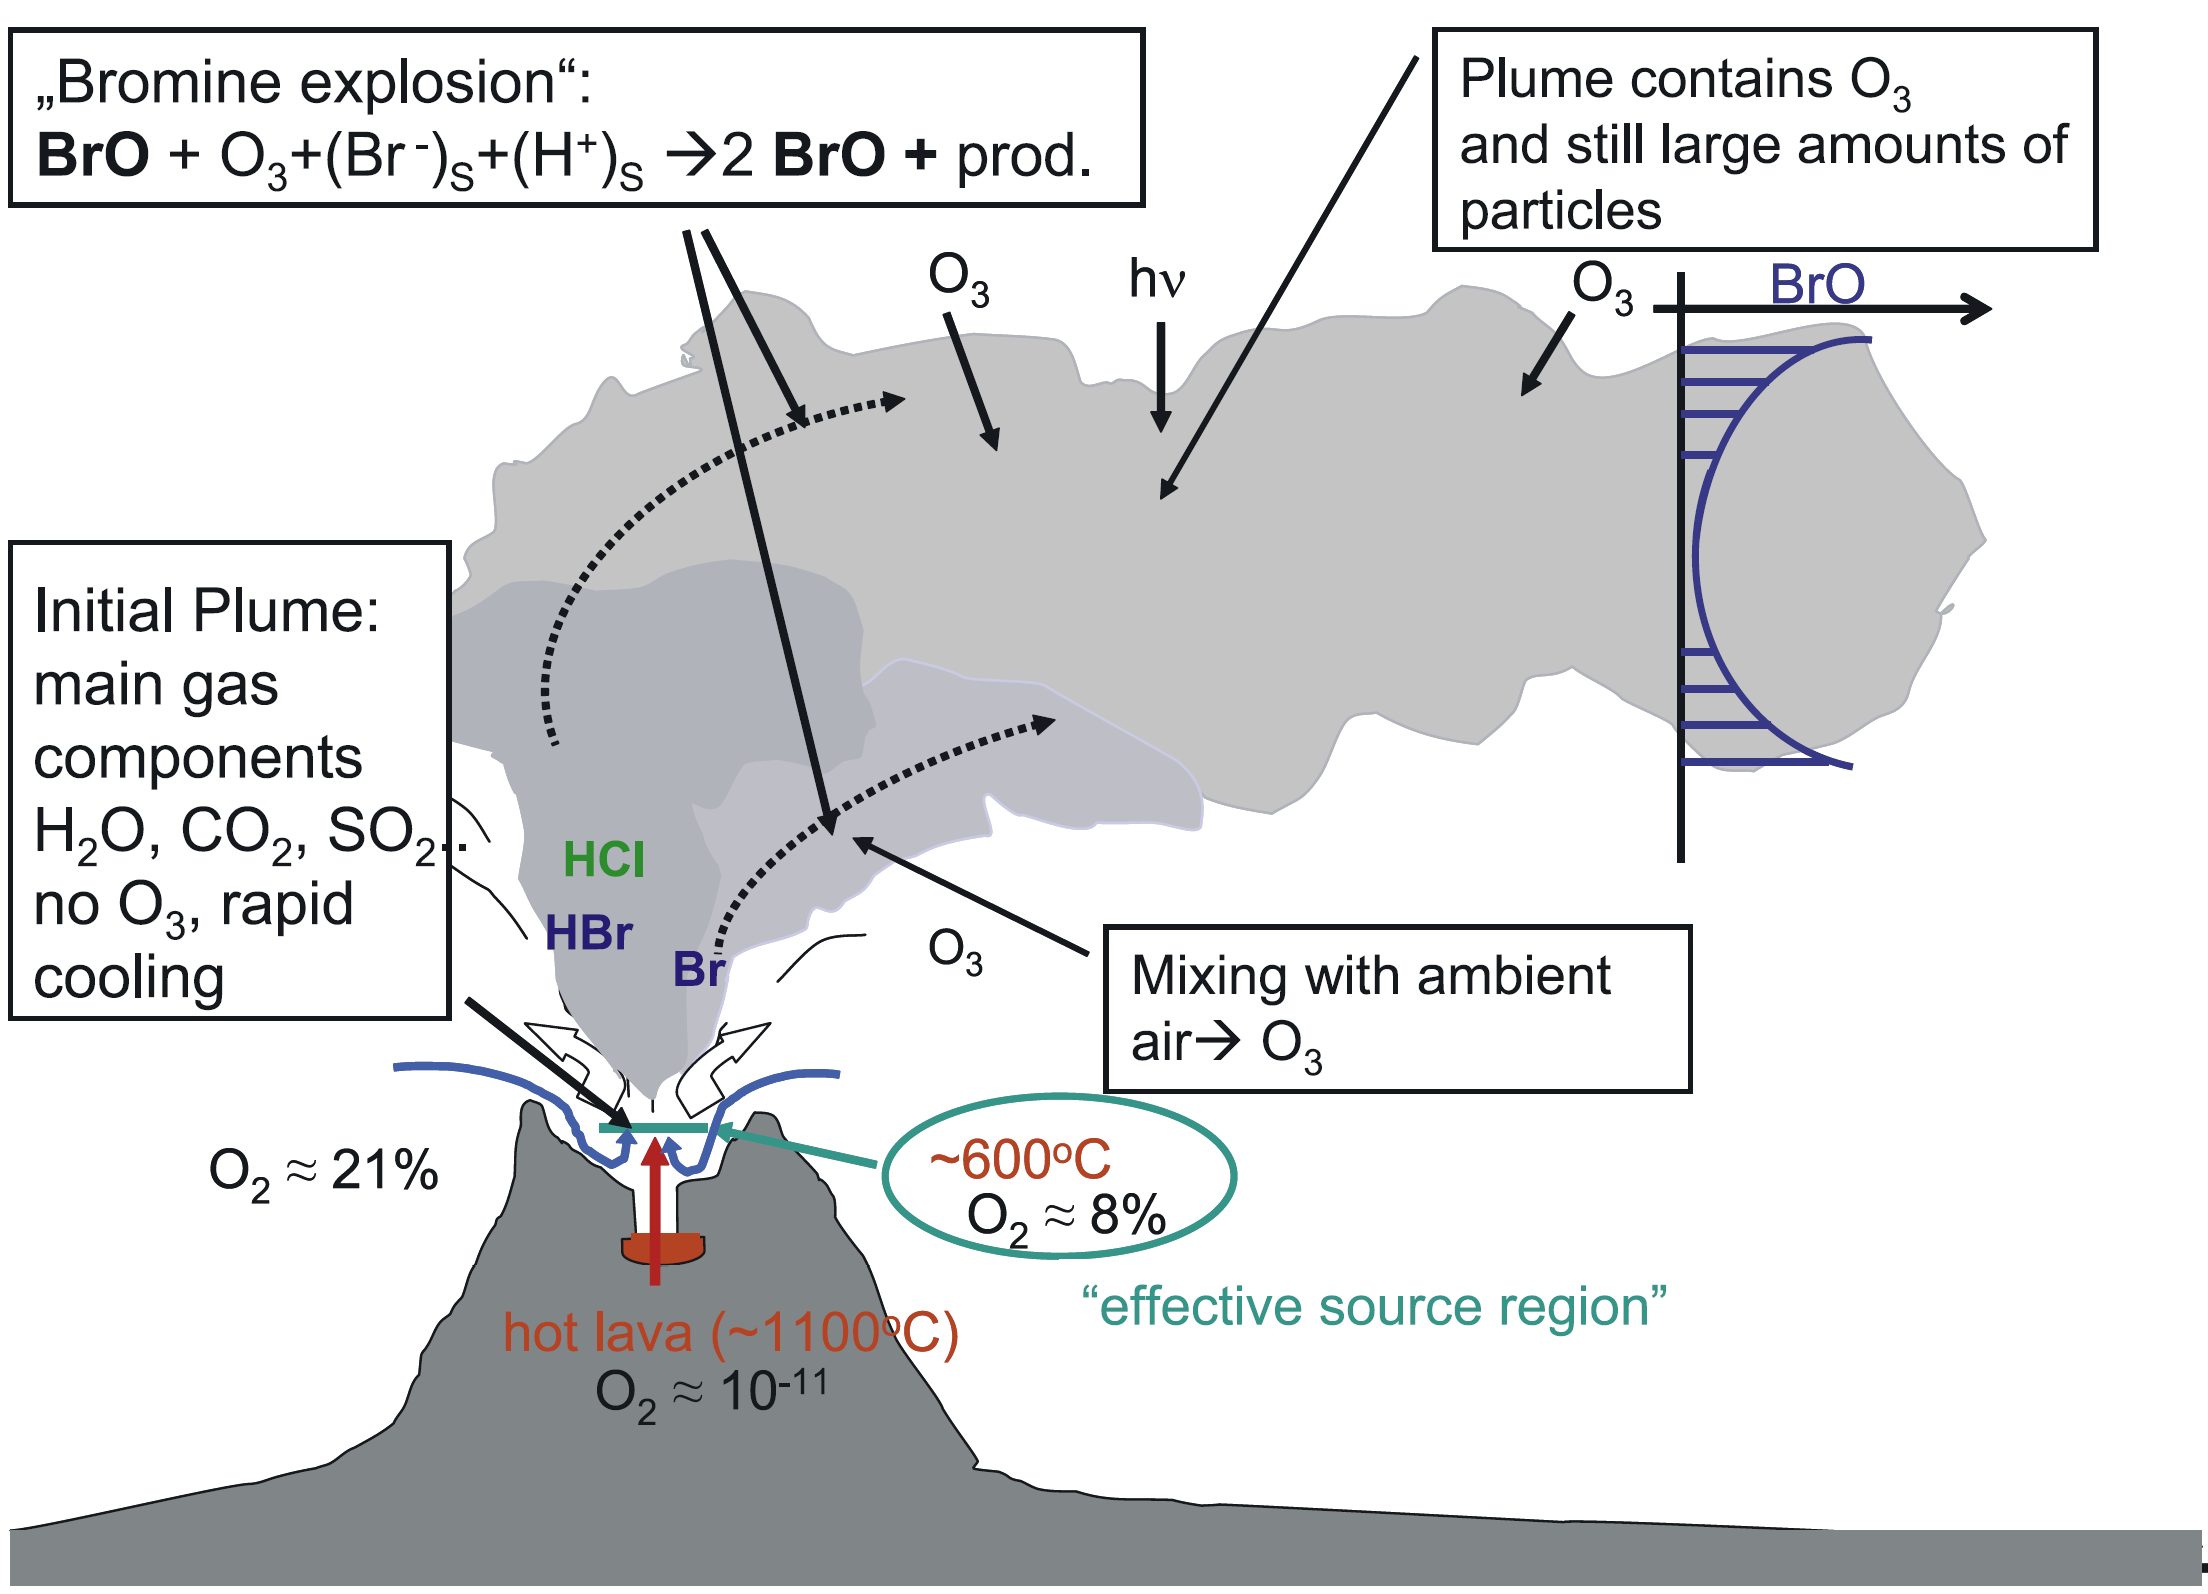
\includegraphics[width=0.9\linewidth]{Bilder/Simon/Bilder_Tung/BrO_Plume}
	\caption{schematic sketch of a Bromine Explosion.
		Release of \ce{HBr} at the volcanic vent. Mixing with ambient air in the effective source region leads to \ce{Br} formation. This resulting Bromine species react to \ce{BrO} with ozone from the plume. Adapted from \cite{bobrowski2007reactive}}
	\label{fig:broplume}
\end{figure}
The amount of Bromine in volcanic plumes is rather low compared to \ce{SO2}. The first time Bromine monoxid (BrO) was observed at a volcano was 2013 at the soufriere hills by \cite{Bobrowski 2013}. Since then many others were able to detect \ce{BrO}  using ground based remote sensing measurement techiques (DOAS: see \Cref{DOAS}) for exampel:
\citet{bobrowski2007so2}, \citet{bobrowski2007reactive},\citet{vogel2011volcanic} and \cite{lubcke2014bro}
\\
The main Bromine formation which is released from the volcano is  \ce{HBr}. \ce{BrO}  is formed due to mixing with the ozone rich atmosphere at ambient temperatures \cite{bobrowski2007reactive}.\\
Due to the raising of hot air in the volcano vent , ambient air is pulled into the vent. There temperatures of  600$^{\circ}C$ to 1200$^{\circ}C$    prevent the formation of \ce{BrO}. Only Br id formed. \ce{BrO}  occures after further cooling and mixing while rising. When the temperature cooles down to ambient conditions the so called "Bromine Explosion" causes a non linear formation of \ce{BrO}.
The "Bromine Explosion" is illustrated in \Cref{fig:broexplosion} and can be described with the following reaction cycle:
\begin{align}
\ce{HBr}_{gas} &\rightarrow \ce{Br}^{-}_{aq} + \ce{H}^{+}_{aq} \label{eq1}\\
\ce{HOBr}_{(gas)} &\rightarrow \ce{HOBr}_{(aq)} \\
\ce{HOBr}_{(aq)} + \ce{Br}^{-}_{(aq)} + \ce{H}^{+}_{(aq)} &\rightarrow
\ce{Br}_{2(aq)} +  \ce{H2O}\label{eq2}\\
\ce{Br}_{2,aq} &\rightarrow \ce{Br}_{2,gas} \\
\ce{Br2} + h\nu &\rightarrow 2 \ce{Br} \\
\ce{Br} + \ce{O3} &\rightarrow \ce{BrO} + \ce{O2} \\
\ce{BrO} + \ce{HO2} &\rightarrow \ce{HOBr} + \ce{O2} \\
\ce{BrO} + \ce{BrO} &\rightarrow 2 \ce{Br} + \ce{O2} \\
\ce{BrO} + \ce{BrO} &\rightarrow \ce{Br2} + \ce{O2}
\end{align}
The gaseous HBr emitted by the volcano is splited heterogeneously int H$^{+}$ and Br$^{-}$ (\cref{eq1}). Inside of an aerosol it forms with HOBr Br2 and H2O (\cref{eq2}). Br2 evaporates to the gaseous phase and splits photolytic  into 2Br .Including an ozon molecule (O3) the two Br react to 2BrO. The last step o the circle visualized in \Cref{fig:broexplosion} with blue lines is the reaction of a BrO with H20 to an HOBrO molecule condensing into the liquid phase  and thuse closing the circle. The non linear explosion occurs due the formation of two BrO particles from one HBr from the volcano.\\
The BrO formation is slightly diminished due to self reaction of BrO molecules marked with the red lines in \cref{fig:broexplosion}. The 2BrO react with themselves and form Br2 or may split photolyticaly into 2Br.\\
THe BrO concentration reaches a maximum approximately 5 minutes after emission and then remains constant for the next 25 minutes \textcolor{red}{hier noch nen Bild} \citet{lubcke2014bro}.
 
\begin{figure}
	\centering
	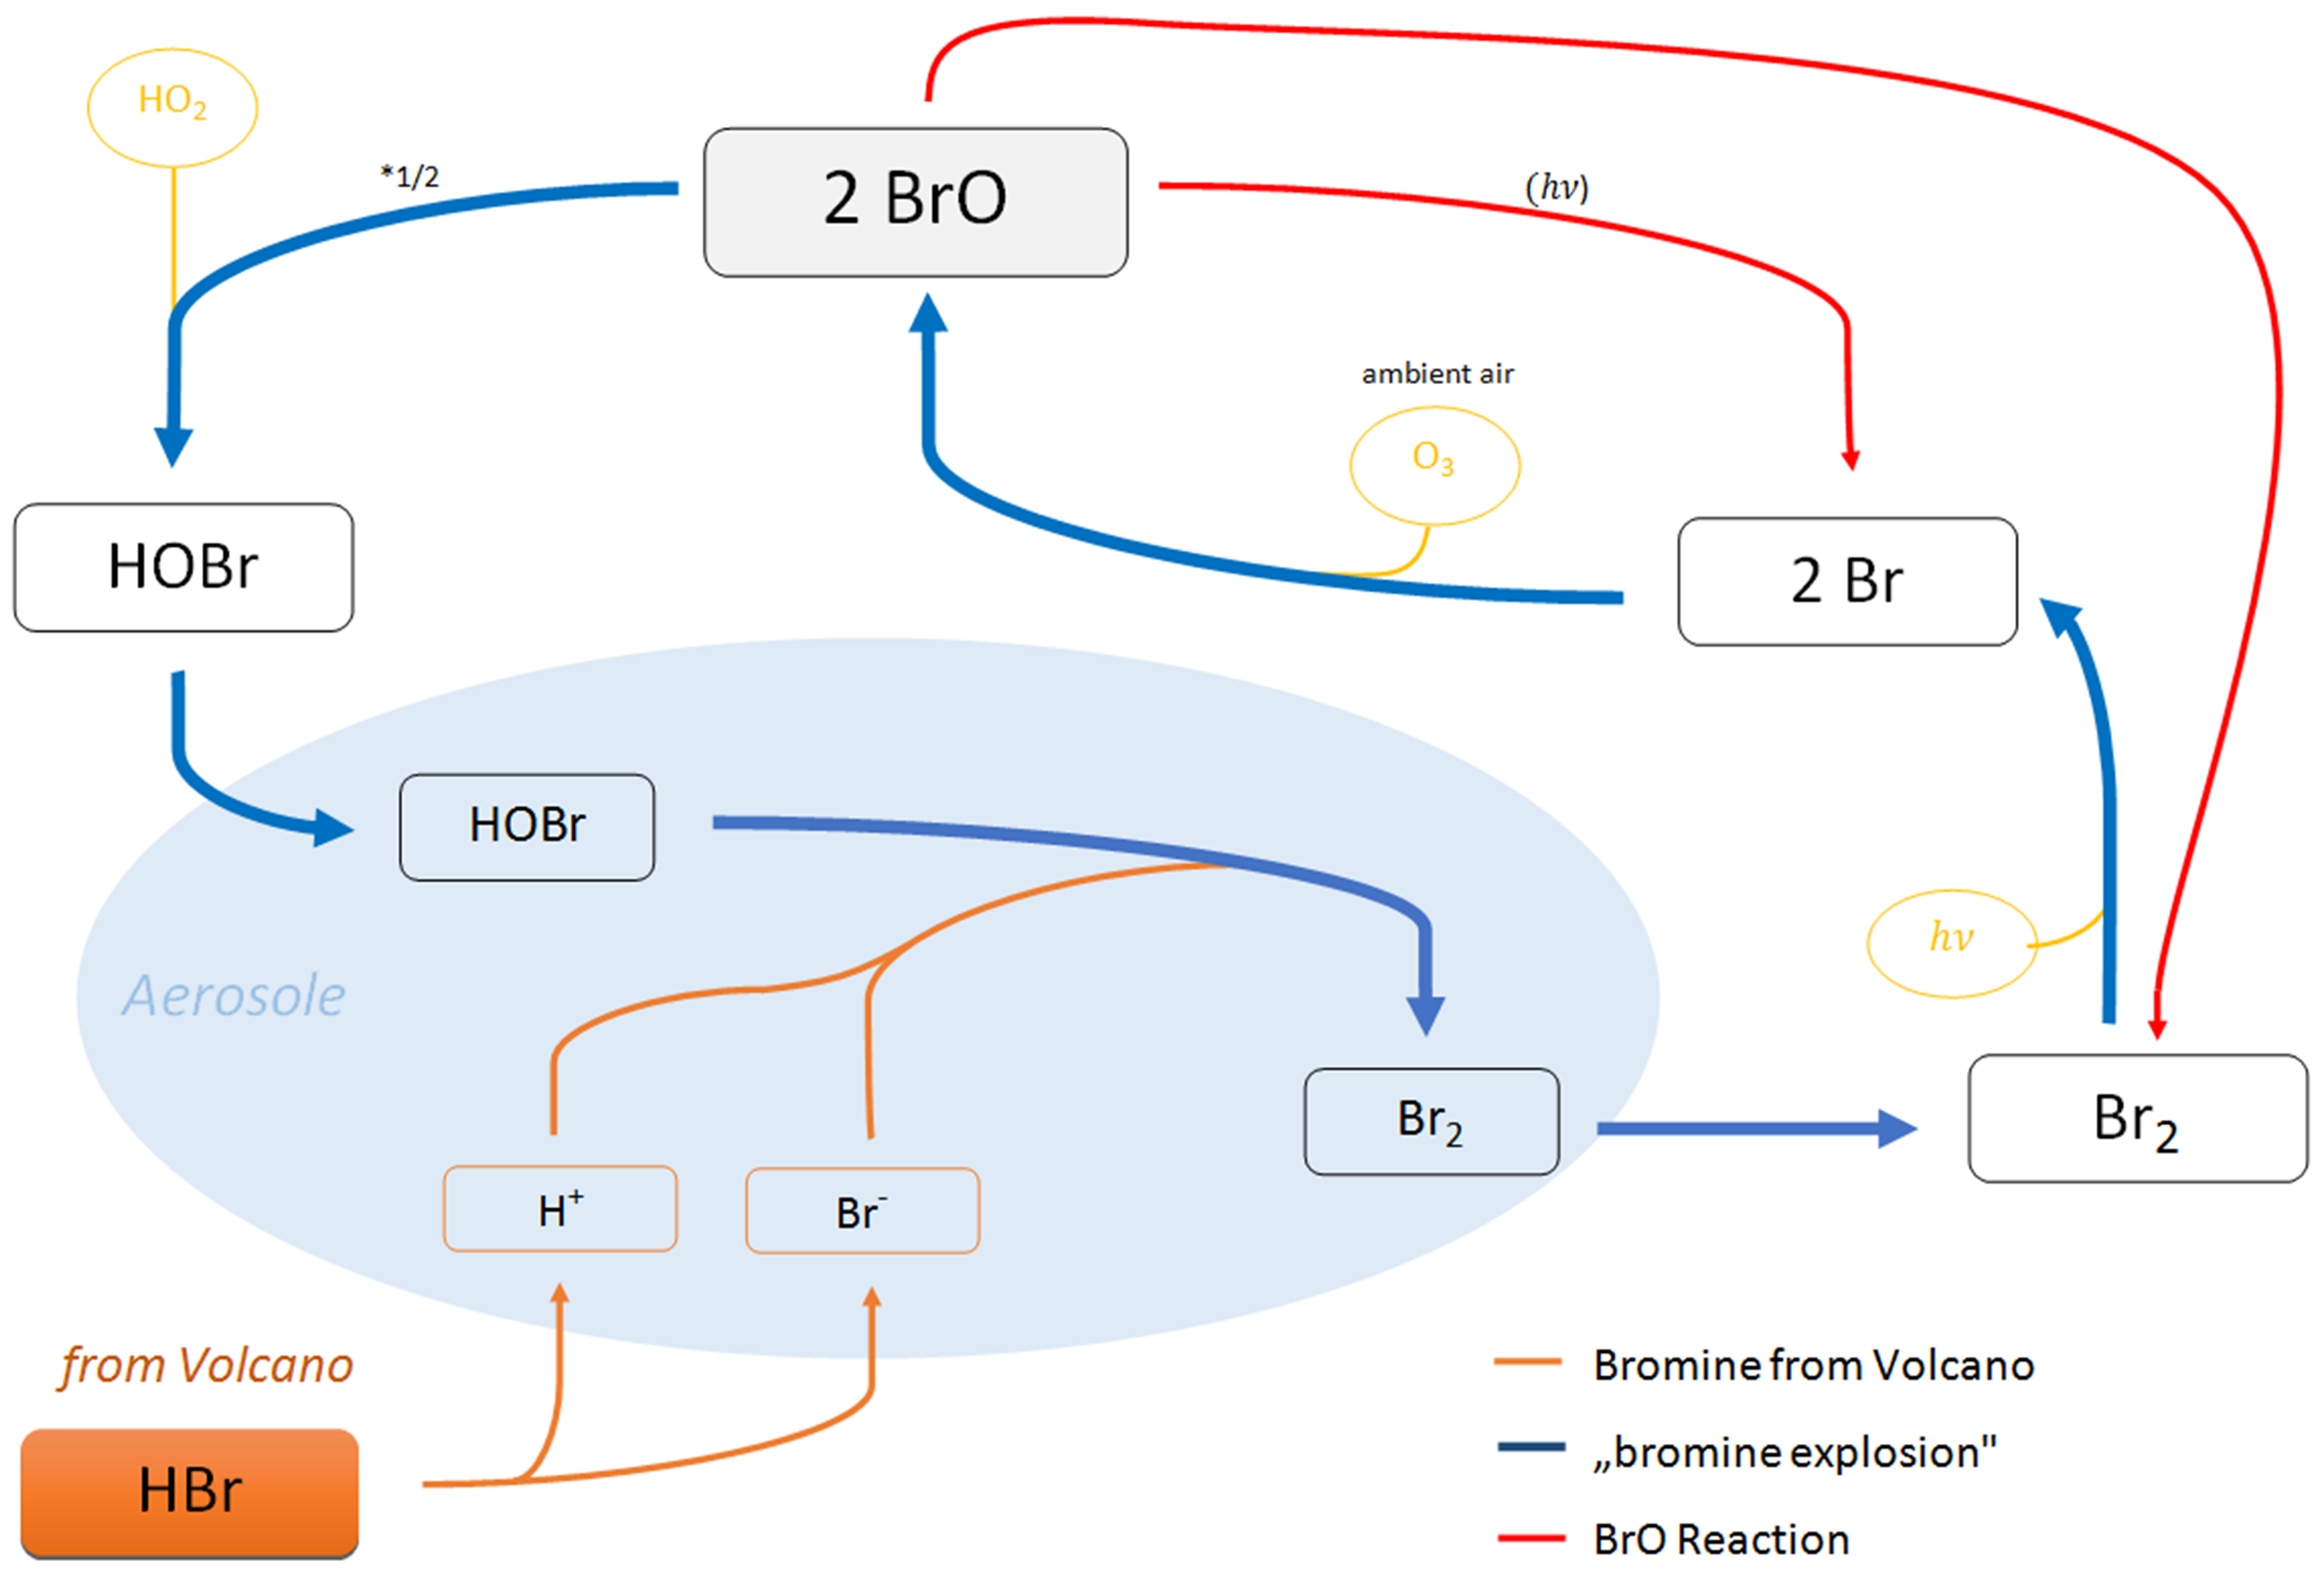
\includegraphics[width=0.9\linewidth]{Bilder/Simon/Bilder_Tung/BrO_Explosion}
	\caption{Bromine reactions inside of a volcanic vent. The release of Hbr at the volcaninc vent is drawn  in orange. Inside of aerosols heterogeneous dissociation with HOBr forms Br2. Then Br2 splits photolytically into single Br radicals. \ce{BrO}  results through a reaction with  \ce{O3}upon mixing with ambient air. Reactions with  \ce{H2O}  forms HOBr creating an autocatalytic cycle. The reaction cycle along the blue lines are called Bromine explosion. From \cite{WarnachSimon}}
	\label{fig:broexplosion}
\end{figure}








\section{Using the \ce{BrO}/\ce{SO2}  ratio to study volcanic activity}
\begin{figure}
	\centering
	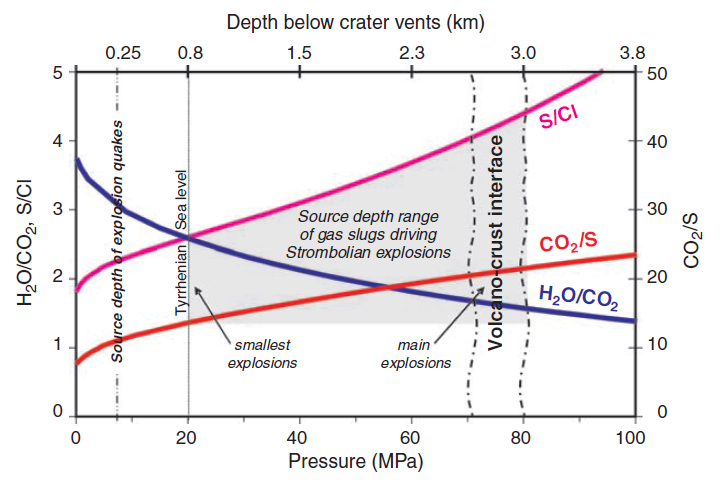
\includegraphics[width=0.9\linewidth]{Zwischenbericht2018/Bilder/so2_bro}
	\caption{Dependency of the ratios of different volcanic trace gases on depth. Data originate from Stromboli volcano. From \cite{lubcke2014optical} reproduced from Burton et al. (2007)}
	\label{fig:so2bro}
\end{figure}    
	
	Volcanic degassing is influenced by many factors, which can be exploit to study volcanic activity by using the gas composition of the volcano plume. Therefore remote sensing should be an additional tool for forecasting of volcanic activity next to classical monitoring techniques like seismographic and deformation measurements.\\
	Inside of volcanoes volatiles are in solution in magmatic melt. The Henry law \Cref{Henrylaw} describes the necessary conditions for gas formation:
	\begin{equation}
	P = K_{H}\cdot c
	\label{Henrylaw}
	\end{equation}
	Here P is the partial pressure at equilibrium of the solute, c is the concentration and $ K_{H}$ is the Henry constant which is anti proportional the the solubility $\alpha$ ($\alpha = \frac{1}{ K_{H}}$).
	If the partial pressure of the gas solute (in this case a magmatic gas constituent) exceeds the pressure of the surrounding solvent, a formation of gaseous bubbles occur. Otherwise, if the partial pressure of the gas in the solution is below the surrounding pressure the formation of gas bubbles stops.\\
	The solubility $\alpha$ depends on the temperature, the chemical composition and on the solvent (here magma). Whereas the partial pressure of the constituent depends on the surrounding pressure. The pressure below the volcanic vent increases with depth, this leads to a correlation between the partial pressure of the constituents and the depth.
	The result is, that the gas starts exsolving at a certain depth depending on the  partial pressure of the constituent. Thus the gas bubble formation increases with rising magma. But at a certain depth the percentage of solved gas is different for each volcanic gas. The result is, that the composition of the gases changes with depth. So gas ratios contain information about its originating source depth.\\
	Prior to volcanic eruptions the magma starts raising since the gas is mostly less dense than the magma it raises faster and could be therefore a indicator for its origin source depth thus a indicator for the volcanic activity.\\
	\Cref{fig:so2bro} shows the ratios of  \ce{H2O} / \ce{CO2},S/CL, \ce{CO2}/S as a function of the pressure respectively on the depth. 
	%
	Especially halogen-sulfur ineresting due to ambient air concentrations are negligible
	%
	Noguchi and kamiya 1963 found decrease Cl/S prior to eruptive periods
	%
	pennisi and le cloarec 1998 lower CL/S ratio during reuptive periods than not erutive periods at etna
	%
	Burton et al 2007 at stromboli  \ce{CO2}/\ce{SO2}  so2/hCl ratios 3-5 times higher during explosions  compaered to quiet degasing
	%
	the authors compared these data to gas formation simulations for different degassing source depth (see fig ..) they concluded that these eruptions were driven by gas slugs from deeper levels where the ratios were higher while quiet degasing originates from from shallow magma
	%
	BrO/\ce{SO2}  curves like in fig .. are not avalible due to lack of  bromine solubility curve but the following observations were made:
	%
	changes of \ce{BrO}/\ce{SO2}  were found by bobrowsky and giuffrida 2012: multiple eruptions between 2006 and 2009 highest ratios 2-3 month before the eruptions the ratio then decreased and was lowest during eruptiv ephase -> bromine exsolved ealyer at lower depth than sulphur 
	%
	lübke found decrease of \ce{BrO}  5 month prior to th eruption 2012 at nevado del ruiz can also be atributed to a earlyer exsolution of bromine during rising magma
	%
	Despite the lack of the solubility curve of \ce{BrO}  until now, the \ce{BrO}/\ce{SO2}  has a great potential for investigations of the volcanic activity. The first reason is, that both gases can be measured with remote sensing by DOAS instruments. For examples ground based measurements by \cite{bobrowski2007reactive}, \cite{lubcke2014optical} ore satelite based measurement by \cite{Hörman et al 2013} or \cite{Beirle at al 2014}. The advanteg of remote sensing techniques is the possibility of measuring during eruptions which is with in situ measurements not always possible.
	Secondly due to the NOVAC network (See \ref{NOVAC}) continues measurements are possible.\\
	Another reason for the research on \ce{BrO}/\ce{SO2}  ratios at volcanoes is the constance of the ratio from 5 to at least 30 minutes after release \citep{bobrowski2007reactive};\citep{lubcke2014optical}. As well as the constance from 5 to 20 km off the volcano see \ref{bild von Simon noch kriegen}. This ensures that the data measured from different positions or at different conditions are comparable.\\
	\\
	This chapter motivated the research on the \ce{BrO}/\ce{SO2}  ratio as a tracer for volcanic activity.
	
	
	
	
	
	
	
	
	
	
	
	
	
	

	\subsection*{Tungurahua \label{Tung}}
	Tungurahua is a subduction zone volcano located in the Ecuadorian Andes (Lat: 01$^{\circ}$,28$^{'}$S; Long:78$^{\circ}$,27$^{'}$W). 2014 Tungurahua was one of the most active volcanoes in southern America, since then the activity was decreasing. Tungurahua is 5023m high and is one of the defining volcanoes of the eastern volcanic rows in Ecuador \citep{hall1999tungurahua}.\\
	Welche daten von welchen zeiten werden angeschaut??\\
	In welcher groeßenordnung sind die gasaustritte in der beochteten Zeit?
		
	\subsection*{Nevado Del Ruiz}
	Nevado Del Ruiz is also a subduction zone volcano. 	Nevado Del Ruiz  is located in the Central Cordillera of Colombia, 140 km west of Bogota.
	(Lat: 04$^{\circ}$,53$^{'}$S; Long:75$^{\circ}$,19$^{'}$W) 
	The hight of Nevado Del Ruiz is 5389 m.
	\\
	Welche daten von welchen zeiten werden angeschaut??\\
	In welcher groeßenordnung sind die gasaustritte in der beochteten Zeit?
	 
	 
	 At Tungurahua three instruments with data recorded in the time span from July in 2008 to August in 2009 are used. Nevado Del Ruiz contributes with two instruments in the time from the end of 2009 to the end of 2011. 
	\chapter{Remote sensing of volcanic gases}
	In this thesis we are interested in the volcanic trace gases \ce{SO2} and \ce{BrO}, both measured with the Differential Optical Absorption Spectroscopy (DOAS) a remote sensing technique proposed by \cite{platt2008differential}\\
	

	\section*{Beer-Lambert Law}
	The Lambert-Beer law describes the attenuation of light when traveling through a material.\\
	This section will give an overview about the reasons for decreasing light intensity when going through a medium.\\
	The Lambert-Beer law describes the attenuation of light when traveling through a material.\\
                                                                                                                                                                                                                                                                                       ,
	Atoms and Molecules exists in several energy states, depending on the different electron configuration. Moreover Molecules have additionally rotation and vibration states, also enclose to the energy states. If a photon matches the energy gap between two possible energy states, this includes, that the lower energy state is occupied and the selection rules are fulfilled  the molecule could absorb the photon, remaining in a higher energy state.\\
	The additional photon energy could be loosed by collision with another molecule or by emission. But since the direction of the emitted photon is mostly not the same direction of the absorbed photon the intensity I$_{0}$ of the light before passing the medium is higher than the intensity I after traveling the distance L through the medium.\\
	This can be described as:\\ 
	\begin{equation}
	I\left(L,\lambda\right) = I_{0}\left(\lambda\right)\cdot expt\left(-\int^{L}_{0}\sigma\left(\lambda,p,T\right)\cdot c\left(l\right)dl\right)
	\end{equation}
	where $c\left(l\right)$ is the location-dependent concentration of the trace gas of interest. $\sigma\left(\lambda,p,T\right)$ is the absorption cross section, $\sigma\left(\lambda,p,T\right)$ is unique for each molecule and depends on pressure p and on the temperature T.\\
	%
	An important quantity used in many optical remote sensing techniques is the optical density $\tau$. The optical density is a measure for the weakening of radiation when going through a material. $\tau$ can be calculated using the lambert beer law:
	\begin{equation}
	\tau = -ln\left(\frac{I\left(\lambda\right)}{I_{0}\left(\lambda\right)}\right) = \sigma\cdot S
	\end{equation}
	Hereby is $S$ the column density. The column density is the concentration of the trace when integrating along the light path, the dimension of $S$ is therefore the number of molecules divided by an area: $\frac{molec}{cm^2}$.
	\begin{equation}
	S = \int_{0}^{L}c\left(l\right)dl
	\end{equation}
	%
	\begin{figure}
		\centering
		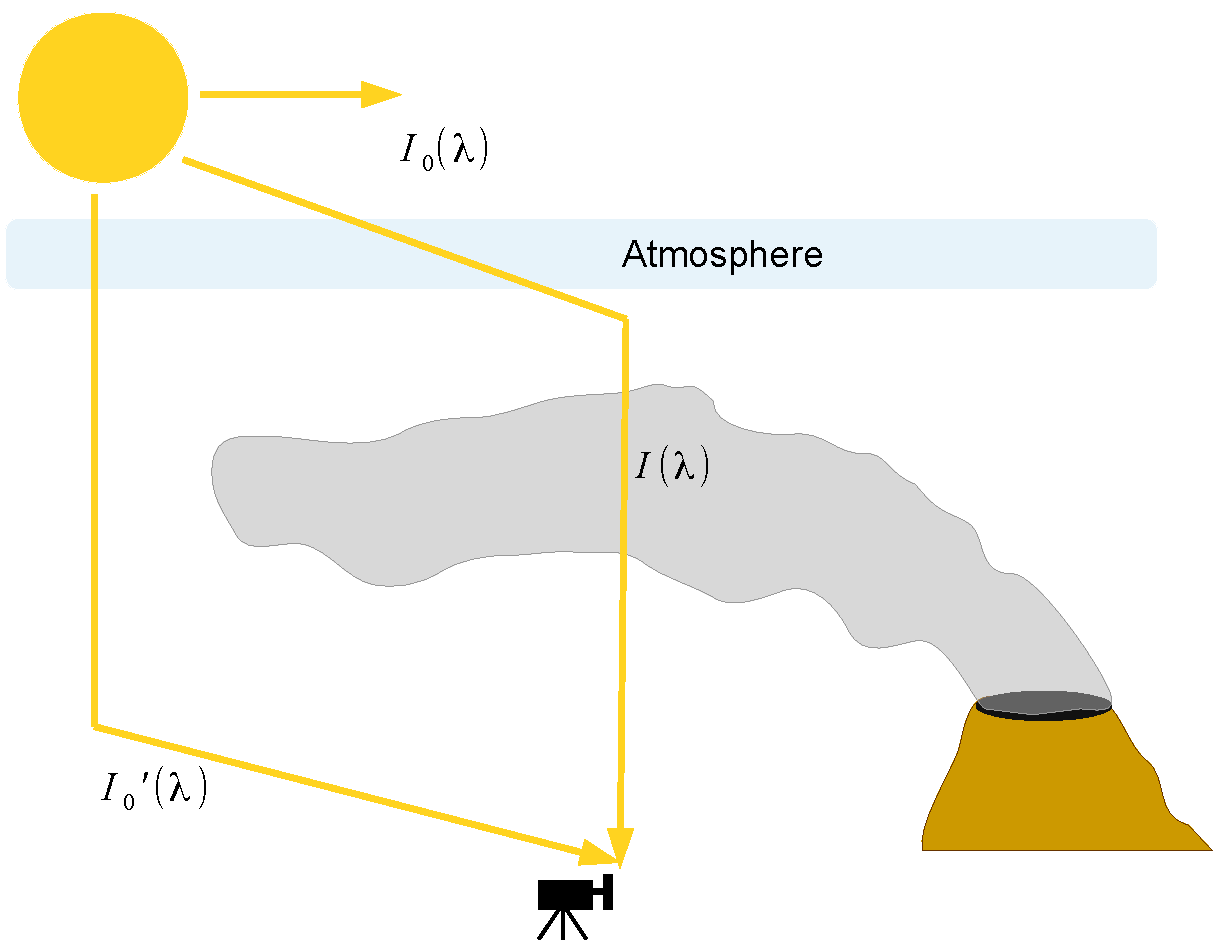
\includegraphics[width=0.9\linewidth]{Bilder/DOASFunction}
		\caption{}
		\label{fig:doasfunction}
	\end{figure}
	
	When measuring at a volcano, that means measuring in the atmosphere the situations gets more complex, since we need to deal with several absorbers and scattering processes have to be taken into account. One possibility is to treat scattering effects as pseudo absorbers with the respective extinction coefficients for Rayleigh ($\epsilon_R$) and  Mie ($\epsilon_M$) scattering
	\begin{equation}
	I\left(L,\lambda\right) = I_{0}\left(\lambda\right)\cdot expt\left(-\int^{L}_{0}\sum_{j}\sigma_{j}\left(\lambda,p,T\right)\cdot
	c_{j}\left(l\right)+\epsilon_R\left(\lambda,l\right)+\epsilon_{M}\left(\lambda,l\right)dl\right)
	\label{eq:lbe}
	\end{equation}
	The first term of \Cref{eq:lbe} in the exponential function, multiple absorbers $j$ are considered, the corresponding concentration depends on the position l of the light path.
	The last two terms in describe the extinction due to Rayleigh and Mie scattering in the atmosphere.\\
	Inelastic scattering (for example the Ring effect) and effects due to turbulences in the atmosphere are neglected here.

	\section{Differential Optical Absorption Spectroscopy (DOAS)\label{DOAS}}
		\begin{figure}
			\centering
			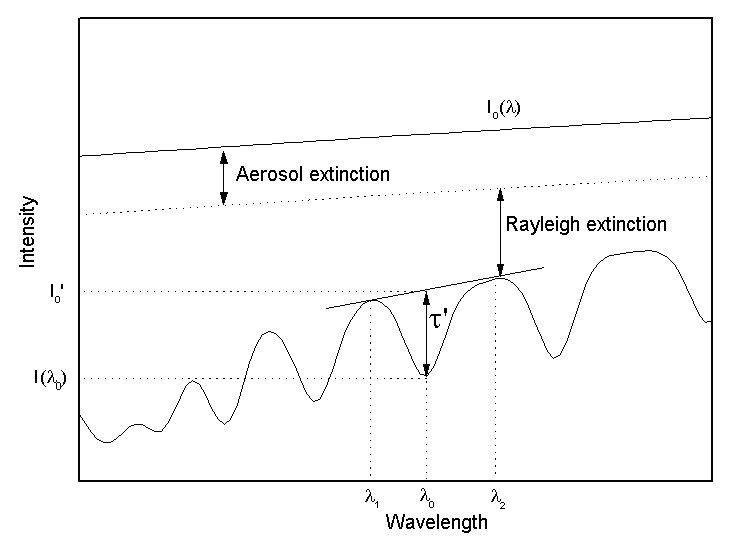
\includegraphics[width=0.8\linewidth]{Bilder/Simon/Bilder_Tung/DOAS_Intensity}
			\caption{Basic idea of the DOAS principle: Light attenuate due to broad band and narrow band effects. The broad band extinction is caused by aerosols and Raylight scattering $\left(I_0\rightarrow I^{'}\right)$. The measured intensity $I$ is formed by narrow band effects due to differential absorption structures by trace gases with the optical density $\tau^{'}$. Adapted from \cite{kern2009spectroscopic}}
			\label{fig:doasintensity}
		\end{figure}
		
	It is impossible to distinguish between various broad-band effects, like scattering in the atmosphere or instrument effects which influence the measured spectra \citep{lubcke2014optical}. Therefore \Cref{eq:lbe} cannot be applied to real measurements.\\
	Differential Optical Absorption Spectroscopy (DOAS) was invented in the late 1970s by \cite{perner1979detection}. This section will give an overview about the DOAS technique. More detailed information ca be found in the work of \cite{platt2008differential}\\
	\newline
	Differential Optical Absorption Spectroscopy uses the fact, that absorption can be divided into broad-band parts and narrow-band parts. Broad band parts are effects that only changes weakly with the wavelength,  i.e. scattering and instruments effects have a broad-band structure. 
	The narrow band part includes effects that strongly depends on the wavelength.
	Within the DOAS-Method only narrow-band absorption features of molecules are used to obtain their column densities.
	The absorption cross section of trace gases $j$ have broad-band ($\sigma_b\left(\lambda \right)$) and narrow band ($\sigma{'}\left(\lambda \right)$) features, only the narrow-band structures are used in DOAS.
	\begin{equation}
	\sigma\left(\lambda \right) = \sigma_b\left(\lambda \right) + \sigma{'}\left(\lambda \right)
	\end{equation}
	%
	With this considerations the Lambert-Beer law \Cref{eq:lbe} can be rewritten
	dividing the exponential part into a narrow-band part and a broad-band part:

	\begin{align}
	I\left(\lambda,L\right) = &\overbrace{I_{0}\left(\lambda\right)\cdot exp\left(-\int^{L}_{0}\sum_{j}\sigma_{b,j}\left(\lambda,p,T\right)\cdot c_{j}\left(l\right)+\epsilon_R\left(\lambda,l\right)+\epsilon_{M}\left(\lambda,l\right)dl\right)}^{=I^{'}_0\left(\lambda\right)} \cdot \nonumber \\
	&exp\left(-\int^{L}_{0}\sum_{j}\sigma_{j}^{'}\left(\lambda,p,T\right)\cdot c_{j}\left(l\right)dl\right)
	\label{eq:bb}
	\end{align}	
		%
	The so defined $I^{'}_0\left(\lambda\right)$ differs from $I_0\left(\lambda\right)$ only by broad band effects. With $I^{'}_0\left(\lambda\right)$ a differential optical density $\tau^{'}$ can be defined:
	\begin{equation}
	\tau^{'} = ln\left(\frac{I^{'}_0\left(\lambda\right)}{I\left(\lambda\right)}\right) = \int_{0}^{L} \sum_{j} \sigma^{'}_{j} \cdot \left(\lambda\right) \cdot c_{j}\left(l\right)dl = \sum_{j}\sigma^{'}_{j}\left(\lambda\right)\cdot S_{j}
	\label{eq:taustrich}
	\end{equation}
	
	The optical density can now be calculated by using the difference of the column density $S_{M}$ in the measurement spectrum to the column density $S_{R}$ of a reference spectrum. From \Cref{eq:bb} we know:	
	\begin{equation}
	I_{P,R} = I^{'}_{0}\cdot exp\left(-S_{P,R}\cdot\sigma\left(\lambda\right)\right)
	\label{eq:smr}
	\end{equation}
	In general the obtained column density $S_{M}$ is called differential slant column density: "dSCD". If the reference spectrum does not contain the trace gas of interest (is not contaminated with trace gases) that means $S_{R} = 0$, $S_{M}$ is called the slant column	density (SCD). 
	With \Cref{eq:smr} the optical density can be derived by:
	\begin{equation}
	\tau\left(\lambda\right) = -ln\left(\frac{I_{M}}{I_{R}}\right) = \sigma\left(\lambda\right)\cdot\left(S_{M}-S_{R}\right)
	\end{equation}
	%

	
	
	\subsection{Technical implementation of the DOAS approach}
	The theory explained above only describes the ideally situation. In real measurements more problems occur due to instrument limitations inelastic scattering causing the Ring effect and due to impacts of external parameters like temperature.\\
	In the following a short overview about these problems and their consequences for our retrieval is given. Further information can be found in \cite{lubcke2014optical}.\\
	\subsubsection*{Optical and spectral resolution of the spectrometer}
	The resolution of the spectrometer is finite, thus, the detector receives a spectrum $I^{*}\left(\lambda\right)$ which can be retrieved with a convolution of the incident spectrum $I\left(\lambda\right)$ with the instrument function H$\left(\lambda\right)$:
	\begin{equation}
	I^{*}\left(\lambda\right) = I\left(\lambda\right)*H\left(\lambda\right)=\int I\left(\lambda-\lambda{'}\right)\cdot H\left(\lambda-\lambda{'}\right)d\lambda{'}
	\end{equation} 
	For the evaluation all $\sigma_{j}$  of the trace gases of interest need to have the same spectral resolution as the instrument used for recording the spectra. In this work we will use high resolution cross sections and convolute them with the instrument function H:
	\begin{equation}
	\sigma{*}\left(\lambda\right) = \sigma\left(\lambda\right)*H\left(\lambda\right)
	\end{equation}
	The instrument function H can be approximated by using a the spectral lines of an mercury lamp since the width of those lines is only a few pm, they could be treated as delta peaks when comparing it to the resolution of the spectrometers.
	
	\subsubsection*{Effects of the detector}
	The detector only has discrete pixels, therefore a wavelength interval is mapped to a pixel $i$.
	
	\begin{equation}
	I^{'}\left(i\right) = \int_{\lambda(i)}^{\lambda(i+1)}I^{*}\left(\lambda{'}d\right)d\lambda{'}
	\end{equation}
	For the retrieval the relationship between the detector channels and the wavelength of the spectrum need to be known.
	The wavelength to pixel mapping (WMP) for a detector with q channels can be calculated as:

	\begin{eqnarray}
	\lambda(i) = \sum_{k=0}^{q-1}\gamma_{k}\cdot i^{k}
	\end{eqnarray}
	Hereby, is $\gamma_{0}$ a shift of the spectrum and $\gamma_{1}$ is a squeeze (respectively stretch) of the spectrum.
	The wavelength to pixel mapping can be discovered by using a mercury lamp again and compare pixel-position with the well known wavelength of the individual HG-lines of the mercury lamp.\\
	The wavelength to pixel mapping depends on the instrument temperature as well as on the ambient pressure \citep{lubcke2014bro}.
	\subsubsection*{Ring effect}
	As mentioned above inelastic scattering causes the Ring effect (named after Grainger and Ring, 1962).
	The Ring effect is observable through a filling of the Fraunehofer lines in spectra of scattered solar radiation, (e.g. if the sunlight travels through the earth atmosphere). When compared to direct sunlight measurements (e.g. outside of the earth atmosphere).
	(\cite{bussemer1993ring},\cite{solomon1987interpretation}) proposes that the Ring effect is a result of  rotational Raman scattering mainly of
	$O_2$ and $N_2$ in the atmosphere.
	\cite{solomon1987interpretation} suggested to treat the Ring effect as a pseudo-absorber. 


	
	\part{Evaluation of the data of Tungurahua and Nevado Del Ruiz}
	
	
	\chapter{Network for Observation of Volcanic and Atmospheric Change \label{NOVAC}}
	%	
	

%% NOVAC
%% =============
%%
		\begin{figure}[h]
			\centering
			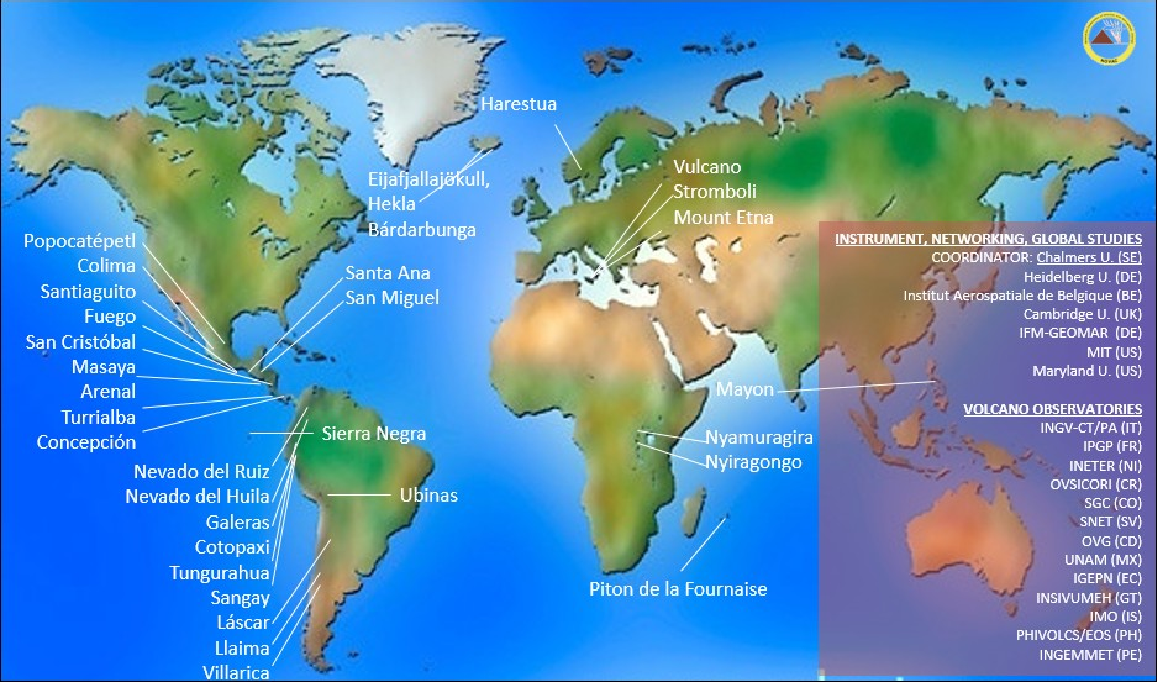
\includegraphics[width=0.8\linewidth]{Bilder/NOVAC2015}
			\caption{Global map of the volcanoes monitored by NOVAC. Used with friendly permission of Santiago Arellano.}
			\label{fig:novac2015}
		\end{figure}
		Network for Observation of Volcanic and Atmospheric Change (NOVAC) is a network of instruments monitoring volcanoes over the whole world. 
		%
		The aim of NOVAC is to gain another tool for risk assessment, for gas emissions and geophysical researches. Also many other scientific purposes are build on the data from NOVAC.\\
		%
		NOVAC was originally funded by the European Union on the first October in 2005. The aim of NOVAC is to  establish  a  global  
		network  of  stations  for  the  quantitative  measurement  of  volcanic gas  emissions. At the beginning, NOVAC encompassed observatories of 15 volcanoes in Africa America and Europe, including some of the most active and strongest degassing volcanoes in the world. Although the EU-funding has stopped, the network has been constantly growing since it was founded. In 2017 more than 80 Instruments are installed at over 30 volcanoes in more than 13 countries.
		\Cref{fig:novac2015} shows a map, with all volcanoes of the Network for Observation of Volcanic and Atmospheric Change.\\
		
		The great advantage of the data monitored in NOVAC is the fact
		that NOVAC provides continues gas emission data over many years. This ensures statistically meaningful results for the data evaluation.\\
		The instruments used in NOVAC are scanning UV-spectrometer named Mini Doas instruments. \\
		The  Mini DOAS  instrument  represents  a  major  breakthrough  in  volcanic  gas	monitoring as it is capable of real-time semi-continuous unattended measurement of the total emission fluxes of  \ce{SO2} and BrO from a volcano. Semi-continues in this case means that the measurement is only possible during daytime when enough Sunlight is there.\\
		%
		\begin{figure}
			\subfigure[Bezeichnung der linken Grafik]{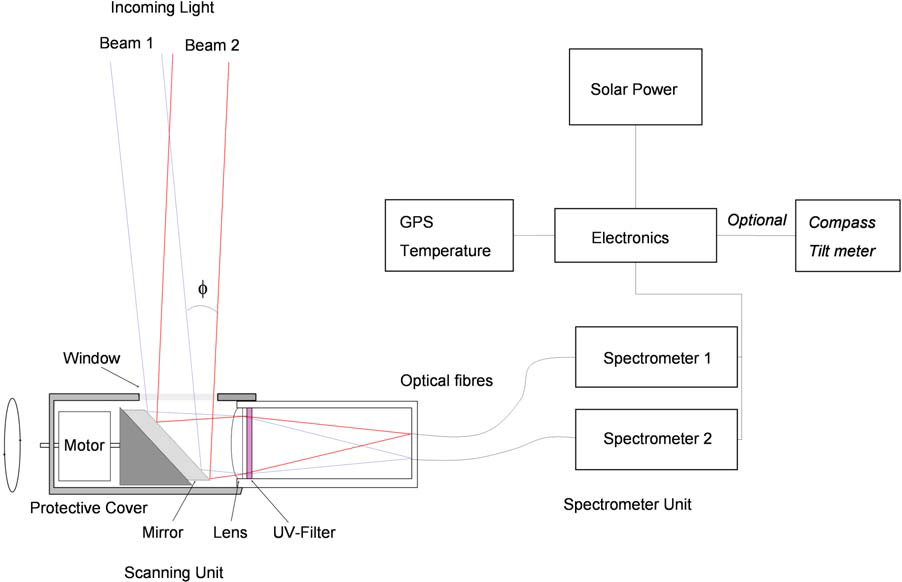
\includegraphics[width=0.49\textwidth]{Bilder/Simon/Bilder_Tung/NOVAC_Instrument}}
			\subfigure[Bezeichnung der rechten Grafik]{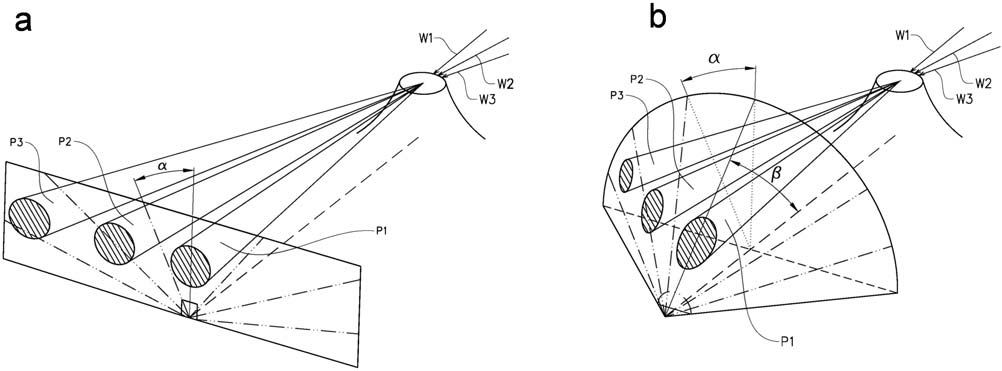
\includegraphics[width=0.49\textwidth]{Bilder/Simon/Bilder_Tung/NOVAC_scan_geo}}
			\caption{Titel unterm gesamten Bild}
		\end{figure}
		The  basic  Mini DOAS  system  consists  of  a  pointing  telescope  fiber-coupled  to  a  spectrograph.  
		Ultraviolet light from the sun, scattered from aerosols and molecules in the atmosphere, is collected by 
		means  of  a  telescope  with  a  quartz  lens  defining  a  field-of-view  of  12~mrad.
		\cite{NOVACsite} \\
		The spectrometers measure in the UV region in a wavelength range of 280 to 420~nm. In this range the differential structures of \ce{SO2} and BrO are dominant.
		\\
		The NOVAC-instruments need to be very robust to stand the conditions around volcanoes. Therefore the design of the instruments is rather simple, this means the instruments do not have internal stabilisation features like temperature stabilization to keep the measurement independent of external parameters.\\
		This comes with a reduced precision of the data, but the huge amount of data produced by NOVAC compensates for this limitation.  
		
		
		\section{Measurement Routine}
		\begin{figure}[h]
			\centering
			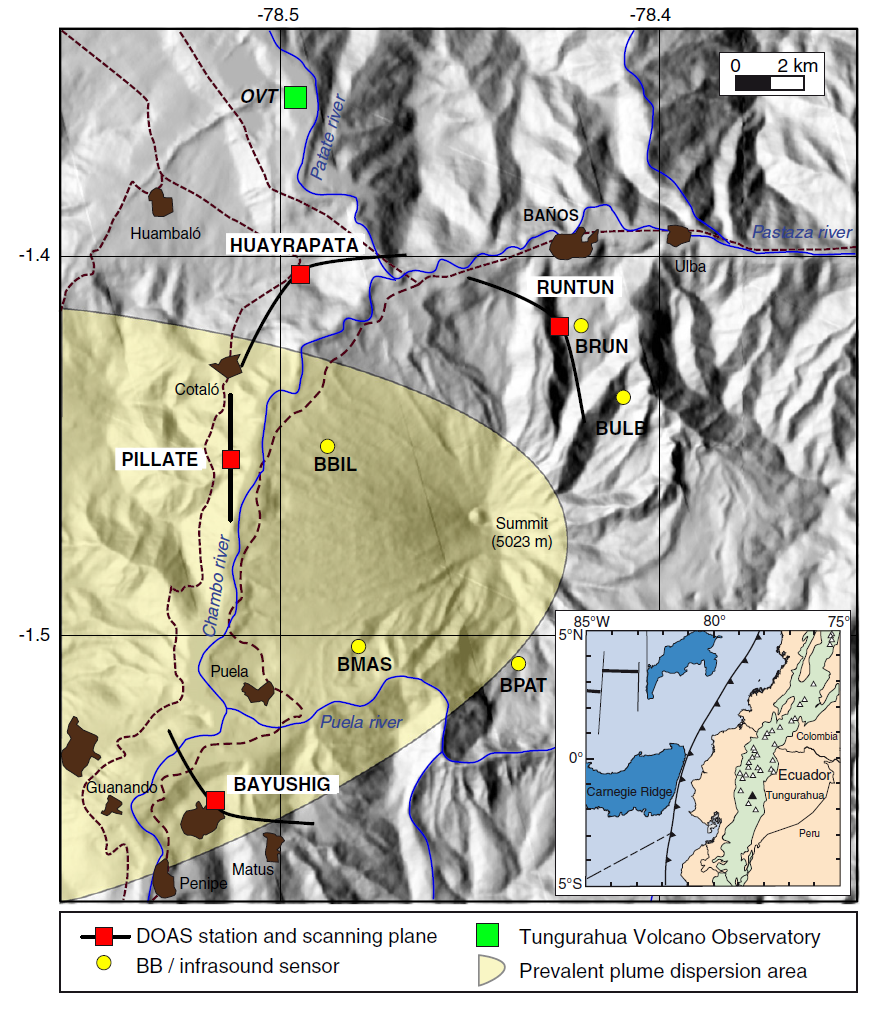
\includegraphics[width=0.6\linewidth]{Bilder/Simon/Bilder_Tung/Map_Tungurahua2}
			\caption{}
			\label{fig:maptungurahua2}
		\end{figure}
		The Instruments are set up five to ten km downwind of the volcano. To cover most of the occurring wind directions two to five instruments are installed at each volcano. Ideally, the measurement plane is orthogonal to the plume, to get the best measurement results. In reality, the measurement plane might be rotated.\\
		The Instruments record spectra in different viewing angles covering a the hole sky from horizon to horizon.\\
		The zenith is at 0$^{\circ}$.
		The measurement routine starts with a spectrum in zenith direction: the pre-reference.
		Afterwards, the dark current spectrum is recorded.\\
		Then the Instrument turns automatically to the side, recording spectra at the elevation angle from -90$^{\circ}$ to 90$^{\circ}$ with steps of 3.6$^{\circ}$. \\
		One hole measurement takes 6 to 15 minutes.
	
	\chapter{Evaluation routine}
	

%% NOVAC
%% =============
%%
This chapter outlines the algorithm which is used for the evaluation of the spectroscopic data recorded in NOVAC. 
The problem of contamination of the reference is explained and possible solutions are presented.

\section{Conventional evaluation routine}
The fitting routine used for this thesis is based on the DOASIS software \citep{kraus2006doasis}. 
The equations of the DOAS retrieval of this work are slightly different from \Cref{eq:taustrich} and therefore described in the following.
\Cref{eq:lbe} can be rewritten as:
\begin{align}
ln\left(I\left(\lambda, L\right)\right) = &ln\left(I_0 \right) + P \left(\lambda\right) -	\int_{0}^{L}\sum_{j}\sigma_j \left(\lambda, p, T \right) \cdot c_j \left(l\right)dl \nonumber \\
= &ln\left(I_0 \right) + P \left(\lambda\right)-
\sum_{j}\sigma_j \left(\lambda, p, T \right) \cdot S_j
\label{eq:lben}
\end{align}
%
The polynomial $ P \left(\lambda\right)$ accounts for all broad-band effects which approximates the scattering effects of the atmosphere as well as broad band absorptions.

The task of the DOAS retrieval is to find a model function $F \left(\lambda\right)$ that minimizes $\chi^2$:
\begin{equation}
\chi^2 = \sum_{i=\lambda_1}^{\lambda_2}\left(ln(I(i))-F(i)\right)^2
\label{eq:Chi}
\end{equation}
While $F\left(\lambda\right)$ can be expressed on the basis of \Cref{eq:lben}:
\begin{equation}
F\left(\lambda\right) = ln\left(I_0 \right) + P \left(\lambda\right)-
\sum_{j}\sigma_j \left(\lambda\right) \cdot S_j
\label{eq:F}
\end{equation}
The DOAS fitting routine uses a combination of a standard least-squares fit and a Levenberg-Marquard algorithm to minimize $\chi^2$\\
\\
Prior to the DOAS fitting. the spectra need to be calibrated, this done by using a wavelength to pixel mapping function (WMP) developed by \citet{lehman 2014}. The WMP uses a solar atlas spectrum that is concolced with the Hg line of the single instruments, hereby am initial calibration based on the Hg lines is given as a first parameter. The calibration is done by fitting the Fraunhofer lines of the recorded spectrum on the convolved Solar Atlas spectrum. The Rayleigh scattering is considered by adding a Ring spectrum as well as a wavelength dependent Ring spectrum (proportional to $\lambda^4$) \citep{wagner2009}. Mie scattering and broadband absorption structures were accounted due to adding a third order polynomial to the retrieval well as an offset polynomial to correct for stray-light influence \citep{lubcke2014bro}.\\
The \ce{SO2} evaluation is performed for a wavelength range between 314.8~nm and 328~nm. Including a \ce{SO2} absorption cross section recorded at a temperature of 298K \citep{vandaele2009fourier} and a  \ce{O3} absorption cross section recorded at 221K \citep{burrows1999atmospheric}.\\
The \ce{BrO}  evaluation is performed for a wavelength range between 330.6~nm and 352.7~nm (found by \citet{vogel2011volcanic}). The sum in \Cref{eq:F} includes for the BrO evaluation the following absorption cross sections:
\ce{BrO}  at 298K \citep{fleischmann2004new}, the \ce{SO2} and  \ce{O3} absorption cross sections described above, \ce{O4} \citep{hermans2003absorption},  \ce{NO2} at 298K \citep{vandaele1998measurements} and  \ce{CH2O} at 298K \citep{meller2000temperature}.\\
%
The choice of the wavelength range as well as the considered trace gases used in the fits is based on studies on the optimal evaluation wavelength range in a combination of real measurement data and theoretical studies for BrO and SO2, made by \citet{vogel2011volcanic}.\\
The spectra of the trace gases were convoluted by using the 334.15 nm line of a mercury lamp.\\
A further effect influencing the evaluation is the $I_{0}$ effect, in order to account for the I0-effect \citep{platt2008differential} an
iterative approach was used. Further informations can be found at (Wagner et al., 2002), \cite{lubcke2014bro},\cite{vogel2011volcanic}).
To further correct for small inaccuracies of the WMP, the FRS and both Ring spectra as one set, and all trace gases absorption cross sections as another set, are allowed to be shifted, and first order squeezed against the measurement spectrum.\\
%
NOVAC provides spectral data for roughly 50 different elevation angles. For the DOAS evaluation a reference and a measurement spectrum is needed. Obtaining the complete amount of volcanic gases is only possible in the case of the availability of references which are free of volcanic gases of interest(this will be discussed more detailed in \Cref{Chap:Cont}). The column density of  \ce{BrO}  and \ce{SO2} of the measurement spectrum relatively to the reference spectrum can be calculated \Cref{eq:Chi} and \ref{eq:F}. \\
\\
\begin{figure}
	\subfigure[]{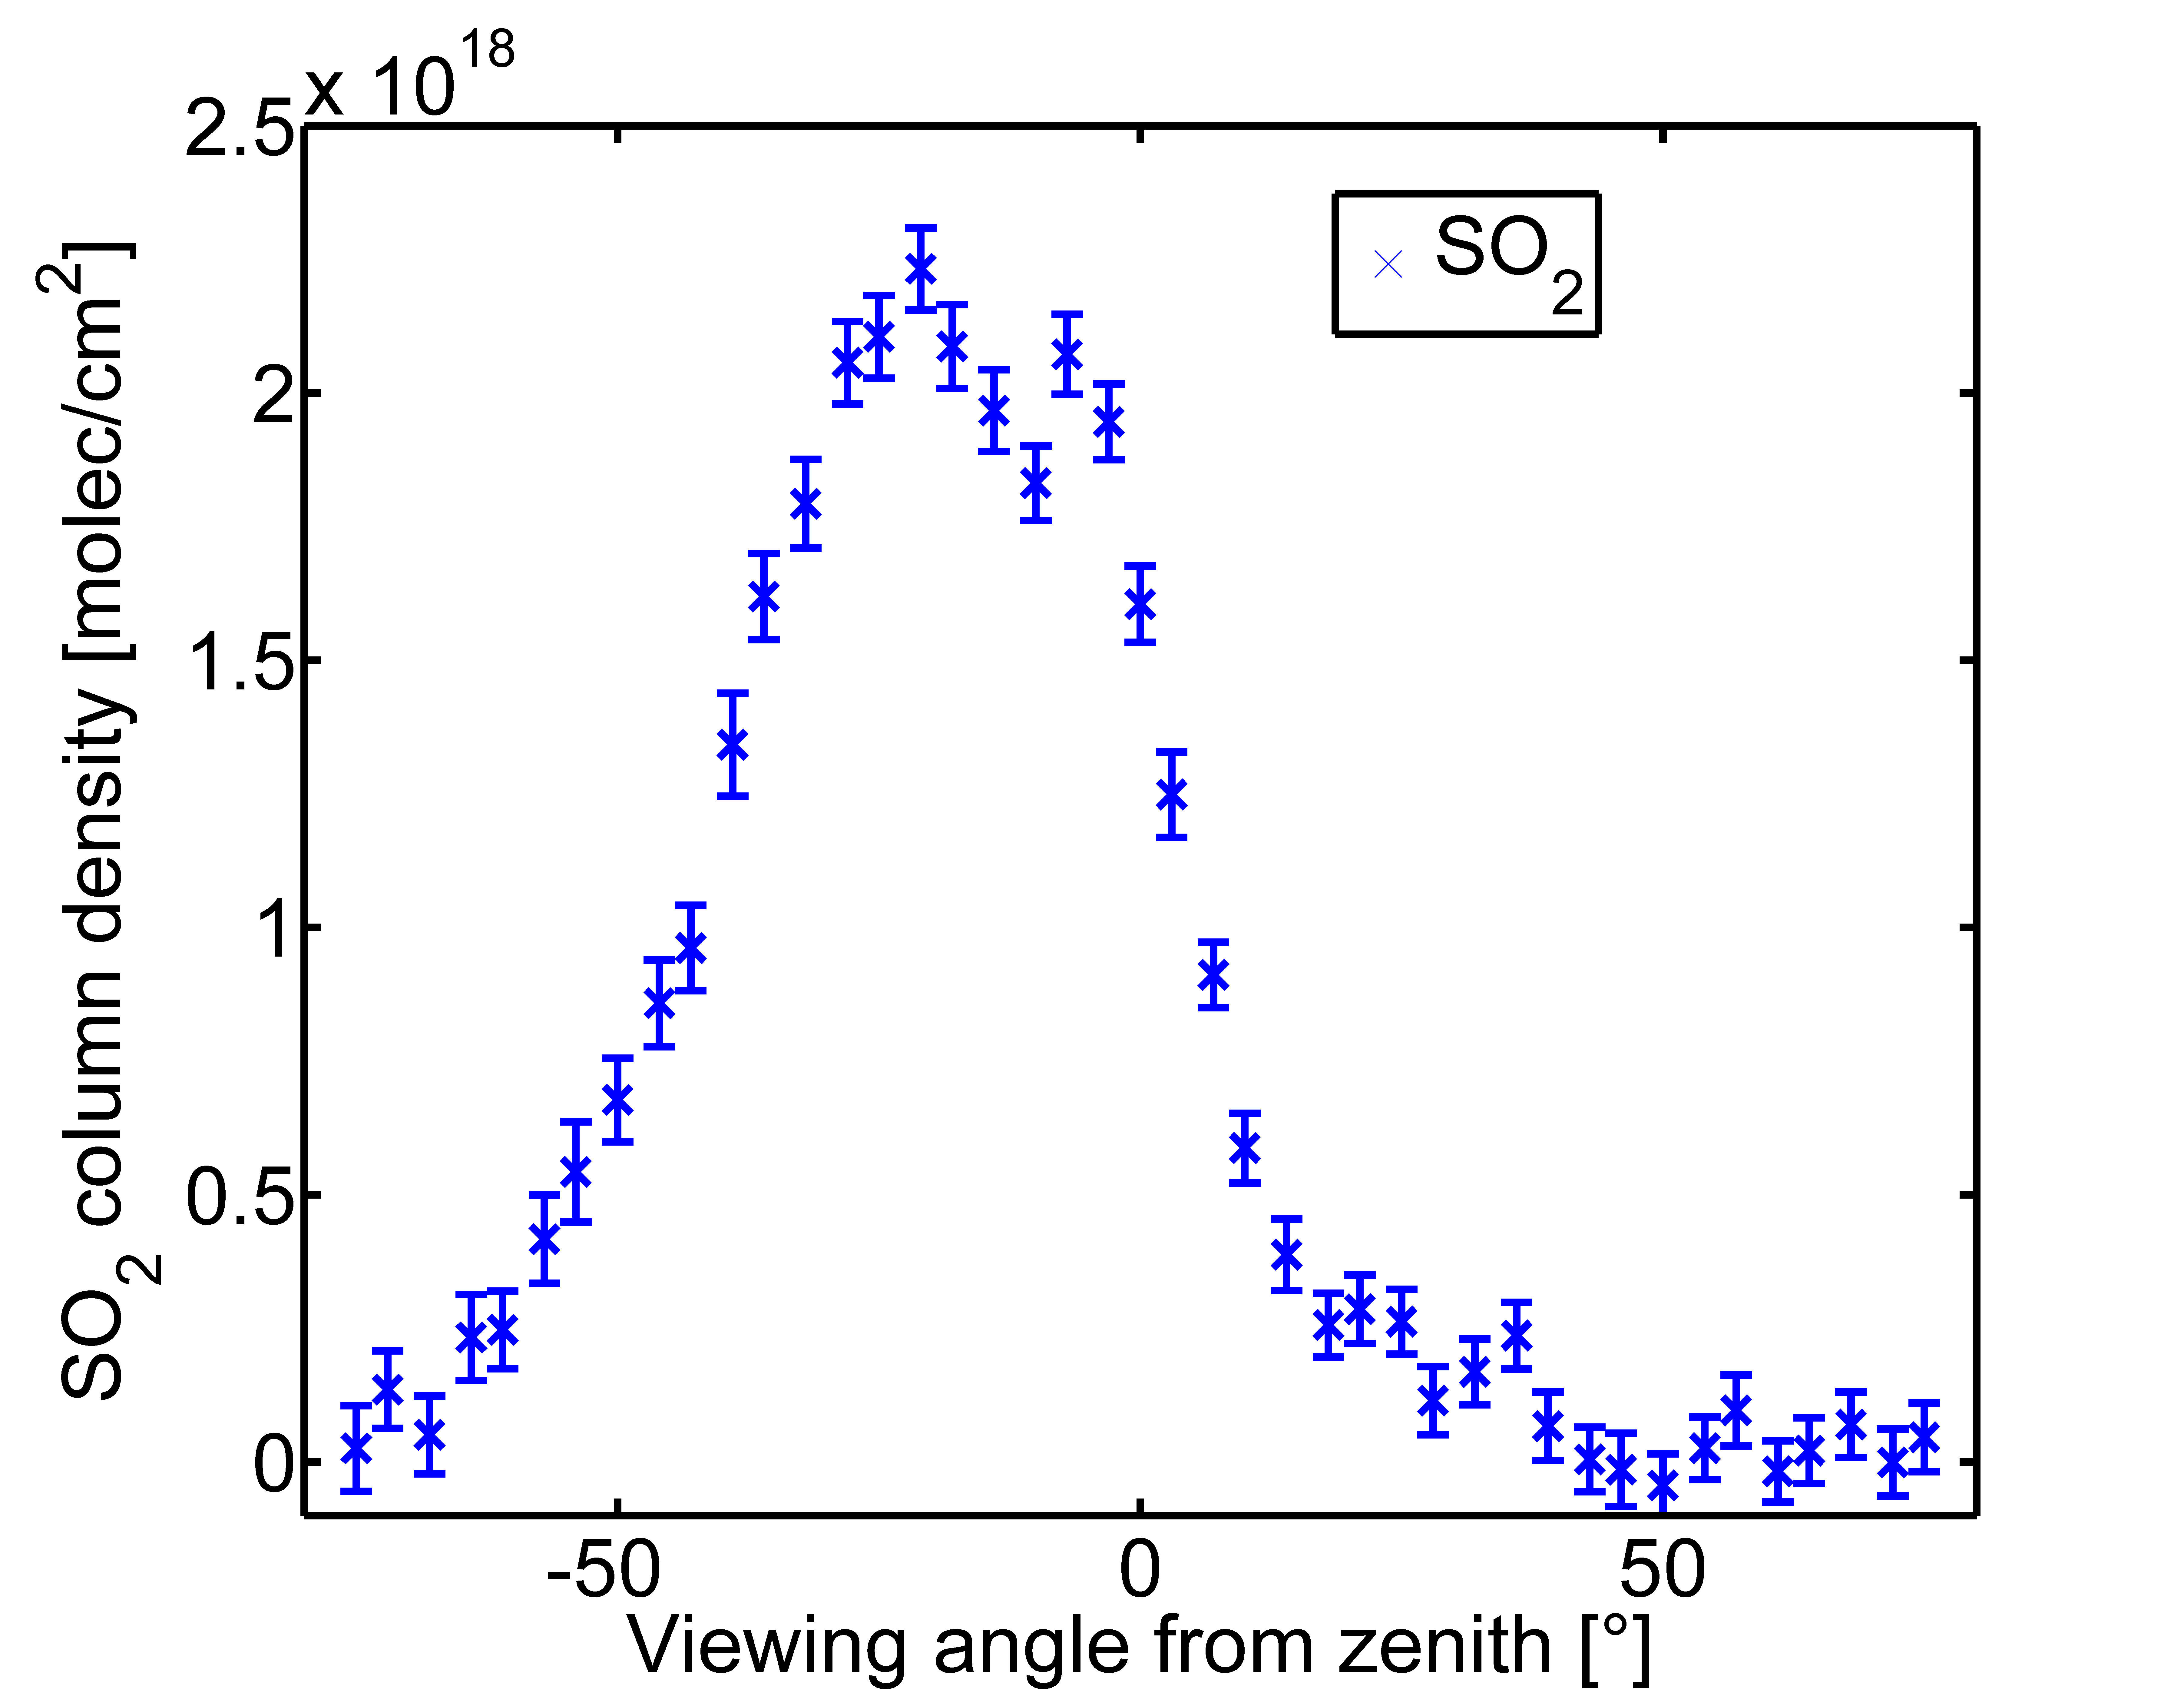
\includegraphics[width=0.51\textwidth]{Bilder/Simon/Bilder_Tung/SO2_Scan_0}}
	\subfigure[]{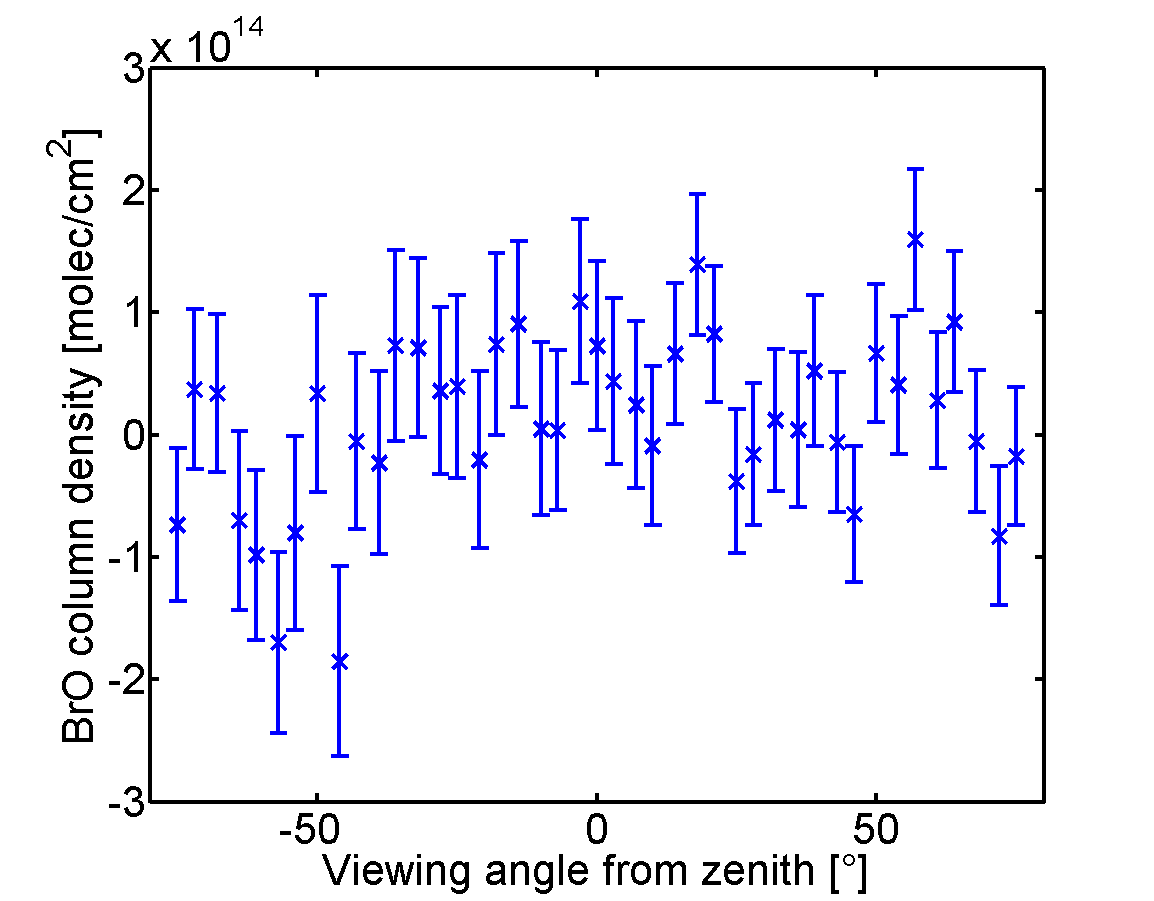
\includegraphics[width=0.51\textwidth]{Bilder/Simon/Bilder_Tung/BrO_Scan}}
	\caption{(a) \ce{SO2} SCD as a function of the elevation angle with error bars computed by the DOASIS fitting routin. (b) \ce{BrO} SCD as a function of the elevation angle with error bars computed by the DOASIS fitting routine.  Taken from \cite{WarnachSimon}}
	\label{fig:plumeref}
\end{figure}
%
In the following we describe the technical implementation of the DOAS approach using the data of NOVAC instruments:\\
%
The first step is to correct each spectrum of the scan for dark current and offset using the dark spectrum.
The next task is to locate the spectra in and outside of the volcanic plume.
First a "pre-reference" (the spectrum recorded at an elevation angle of  0$^{\circ} $) is used to perform the evaluation of the scan spectra recorded at every elevation angle.
For every spectrum of the scan the \ce{SO2} differential slant column density (dSCD) with respect to the pre-reference is calculated using \Cref{eq:F} by the DOASIS fit routine.

The result is \ce{SO2} dSCDs as a function of the elevation angle. This way the elevation angle corresponding to the maximum and the minimum of the \ce{SO2} column density can be determined. The location of the \ce{SO2} maximum defines the location of the plume. The assumption is that the minimum of the \ce{SO2} curve corresponds to a region outside of the plume which is true in most cases. The background \ce{SO2} amount in the earth atmosphere around Tungurahua is usually negligible (see  \Cref{chap:so2}) so we take it as a region of zero \ce{SO2}. \\
We use a gauss fit of the \ce{SO2}-elevation-angle-curve to define the plume region.
%
\begin{figure}
	\centering
	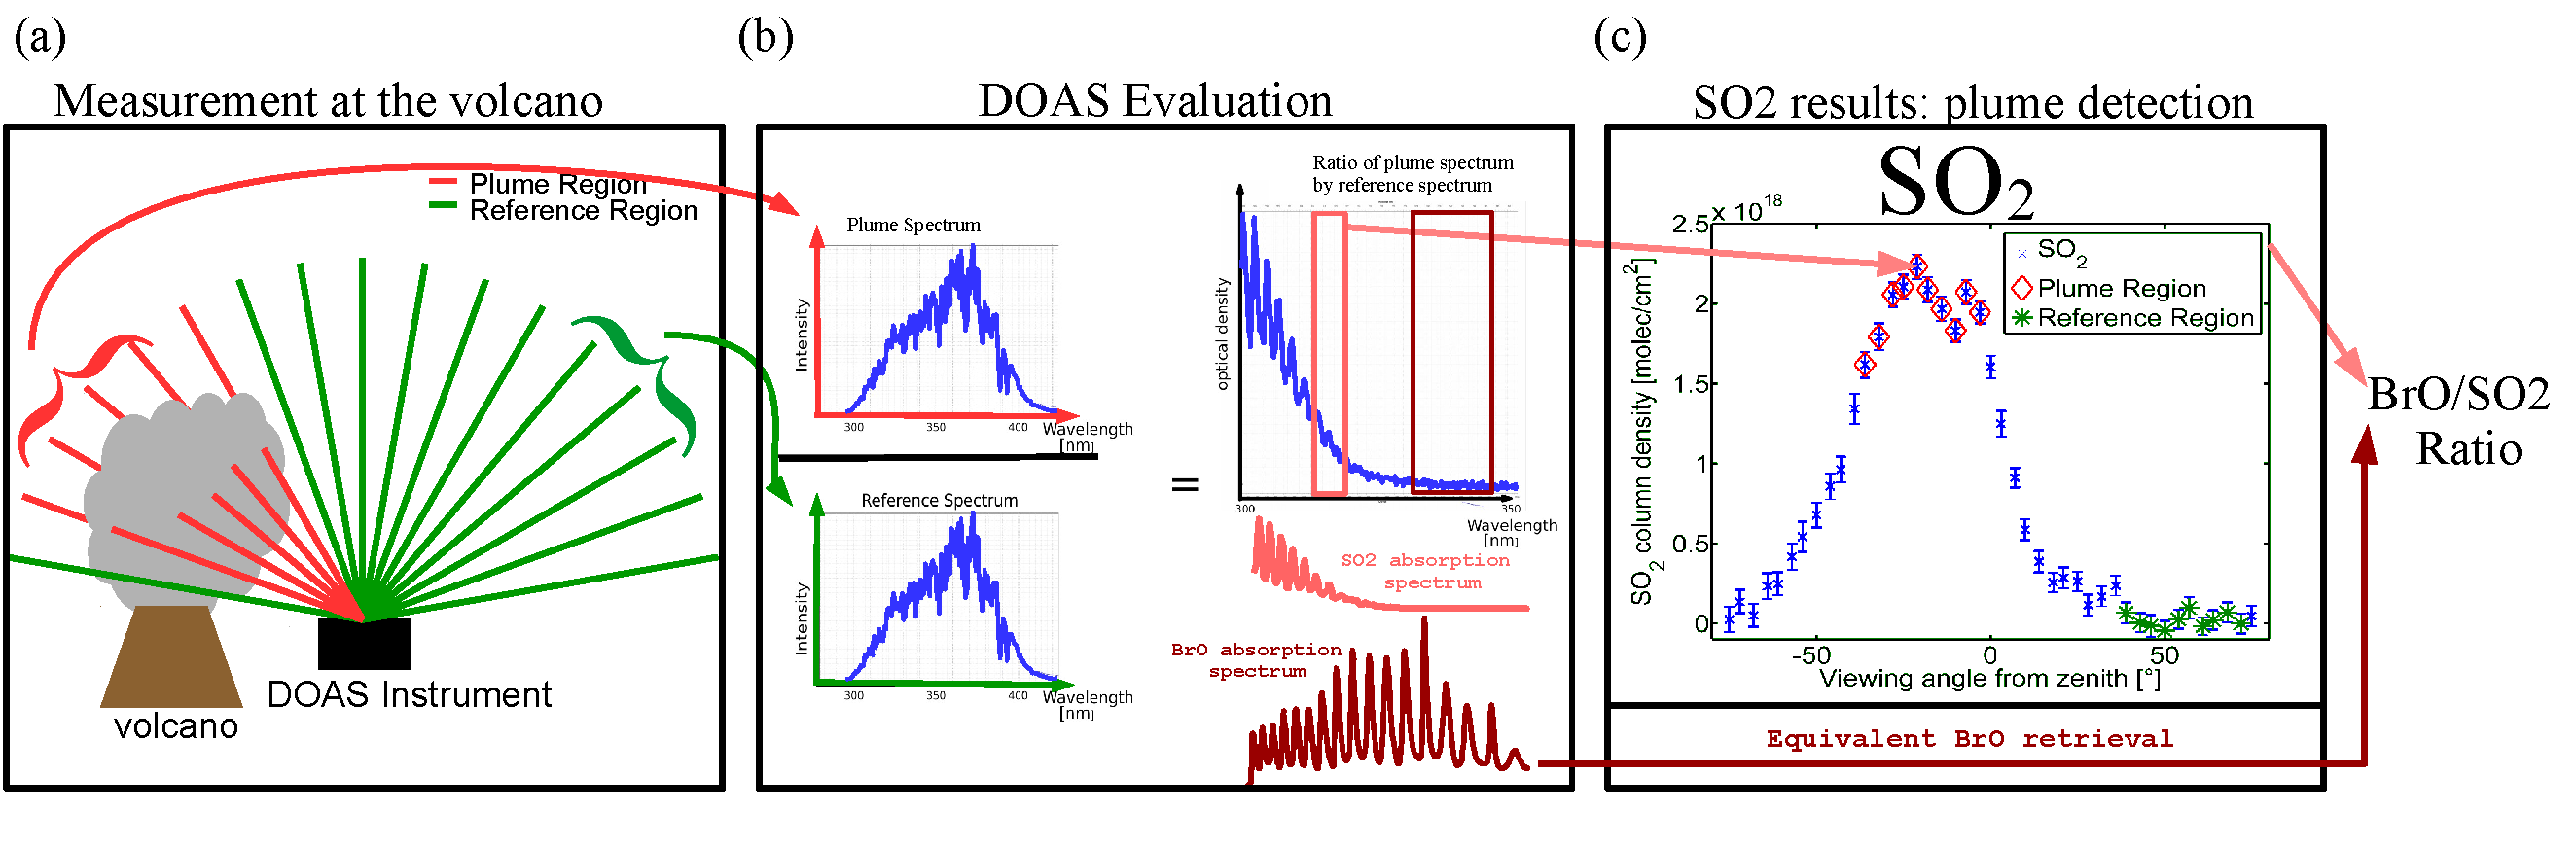
\includegraphics[width=1\linewidth]{Bilder/NOVAC_Eval}
	\caption{NOVAC Evaluation: (a) Measurement at the volcano (b) Evaluation of the spectral data with the DOAS routine using the absorption cross sections of \ce{BrO}  and \ce{SO2}. (c) Finding the location of the plume and reference (taken from \cite{WarnachSimon}) (d) Computation of the ratios BrO/\ce{SO2}}
	\label{fig:NOVAC_Eval}
\end{figure}
The sum over all plume spectra is taken, which are in the elevation angle interval of the gauss peak plus minus one sigma, to increase the photon statistic and to reduce the residuum. If the gauss curve is too wide, what this means in specific is that more then 10 spectra are added within the gauss evaluation, The running mean is calculated and the 10 spectra with the highest \ce{SO2} amount are used for the retrieval. As reference we use the sum of the 10 spectra with the lowest \ce{SO2} amount.\\
The absolute slant column densities (SCD's) of \ce{BrO}  and \ce{SO2} can now be calculated with the previously defined reference and plume spectrum.
In \Cref{fig:plumeref} (a) an example \ce{SO2} SCD as a function of the elevation angle is shown. The \ce{SO2} curve has a maximum at the position of the plume at an elevation angle of approximately $-30^{\circ}$ to $0^{\circ}$  and a reference region at an elevation angle of $40^{\circ}$ to $70^{\circ}$. \Cref{fig:plumeref} (b)  illustrates that  extrema of the \ce{BrO}  curve are not as distinct as it is the case for the \ce{SO2} curve.\\
Since the \ce{BrO} column density is much lower than the \ce{SO2} column density, and just lies slightly above the detection limit, the plume is hard to detect using the \ce{BrO} column density as it is shown in fig. \ref{fig:plumeref} (b). 
Therefore we evaluate BrO only in the plume location determined by using \ce{SO2}.\\
In a further step multiple reference and plume spectra of successive measurements are added to further increase the fit quality.
\Cref{fig:NOVAC_Eval} visualizes the different steps described above in the retrieval of the BrO/\ce{SO2} ratios.\\
\Cref{fig:algorithm} (b) shows the routine of adding multiple spectra of consecutive measuring times. In the following the spectra resulting from the multi adding technique will be referred to as "Multi Add Spectra". The algorithm for co-adding is visualized in \Cref{fig:algorithm} (b) was invented by \citet{vogel2011volcanic} and \citet{lubcke2014bro}.\\
%
Taking the \ce{BrO}/\ce{SO2} molar ratios if the column densities are close to zero yields unpredictable and unrealistic results. Thus, spectra measured in a thin volcano plume need to be excluded.
This could be achieved by setting a \ce{BrO} or/and an \ce{SO2} threshold. A reasonable \ce{BrO} threshold needs to be at least in the order of the DOAS fit error. However this could lead to elevated \ce{BrO}/\ce{SO2} ratios, since the \ce{BrO} error is often close to the detection limit. Thus, all low \ce{BrO} column densities are excluded from the evaluation  \citep{lubcke2014bro}, as an effect the ratios are systematic to high.
%
\begin{figure}
	\subfigure[ ]{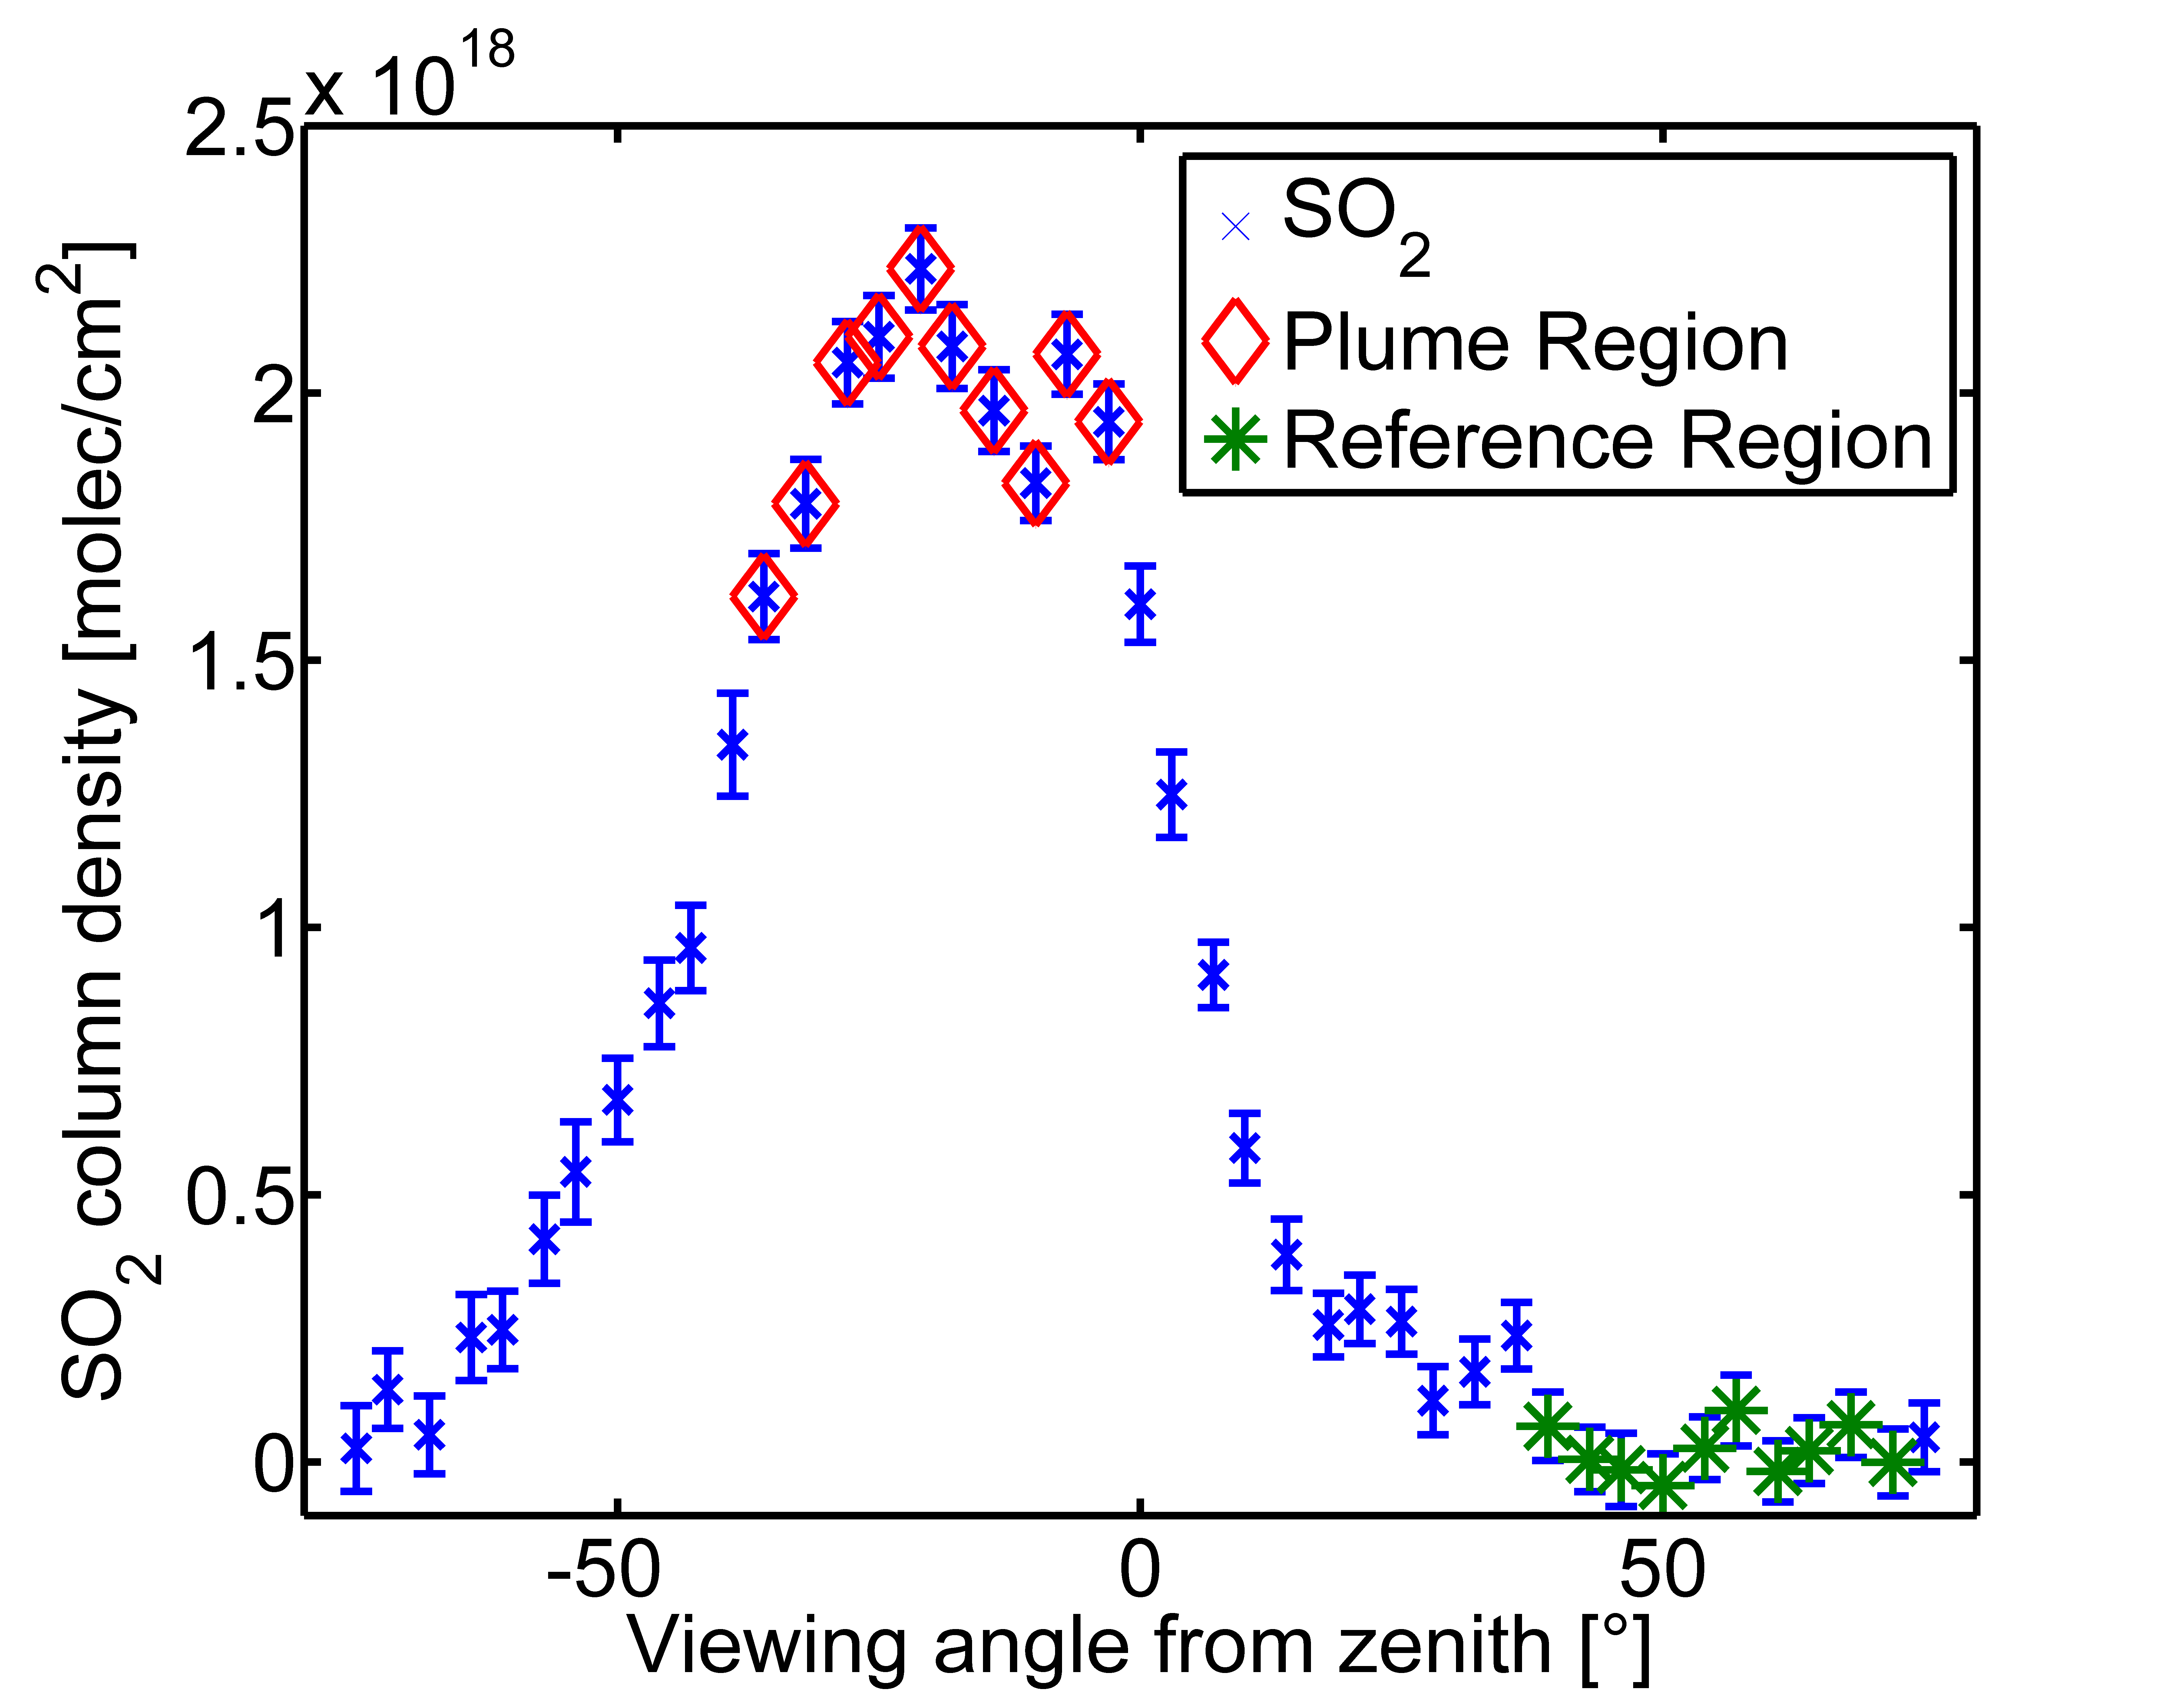
\includegraphics[width=0.53\textwidth]{Bilder/Simon/Bilder_Tung/SO2_Scan}}
	\subfigure[ ]{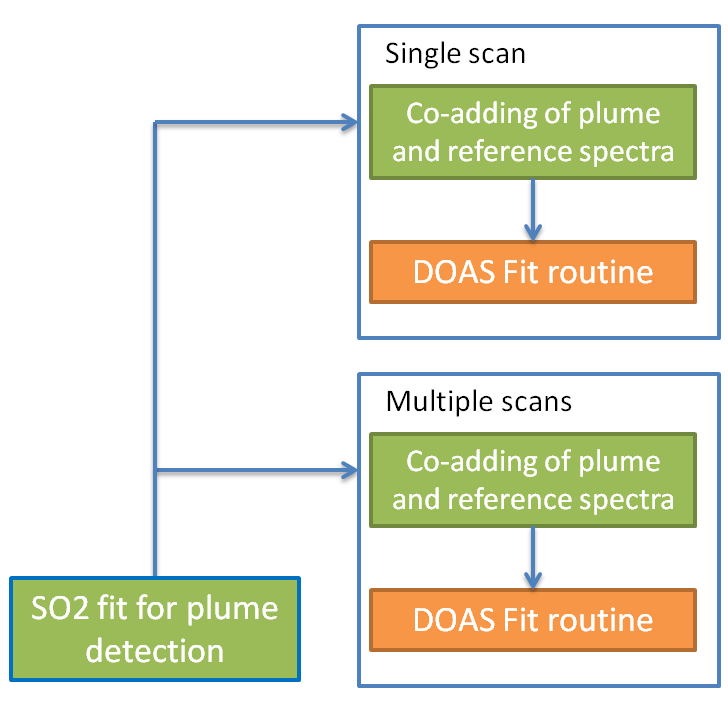
\includegraphics[width=0.47\textwidth]{Bilder/Simon/Bilder_Tung/Algorithm}}
	\caption{(a) \ce{SO2} SCD as a function of the elevation angle. The co-added plume region is marked with red diamonds, and the co added reference region with green stars. From \cite{WarnachSimon}. (b) Flow chart of the \ce{BrO}  and \ce{SO2} evaluation. From \cite{lubcke2014optical}.}
	\label{fig:algorithm}
\end{figure}
The other possibility is to set an \ce{SO2} threshold. In this thesis an \ce{SO2} threshold (plume limit) of $7\cdot 10^{17} \frac{molec}{cm^2}$ is used for the selection of spectra for the evaluation of the \ce{BrO}/\ce{SO2} ratio. $7\cdot 10^{17} \frac{molec}{cm^2}$ is a high threshold for the column density. However, this approach assures that only strongly significant gas amounts are accounted \citep{lubcke2014bro}. Choosing the \ce{SO2} threshold in this way leads to consistent observations for strong degassing, but low degassing events are rather excluded in the evaluation.\\
\textcolor{red}{Ich würde hier noch erwähnen für welche Ratios wir mit diesem Plume Limit sensitiv sind (siehe Appendix in Dinger et al, 2018).}\\
Increasing a plume limit leads to a decrease of usable data. The ratio of usable  data as a function of the plume limit is shown in \Cref{fig:percentageminso2}. An exponential decrease of data can be observed. The plot is based on the data of Tungurahua. Plume limits below 7$\cdot10^{17}$ are shaded in yellow. A plume limit of 7$\cdot10^{17}$ leads to a ratio of usable data of approximately 10\%.
\begin{figure}
	\centering
	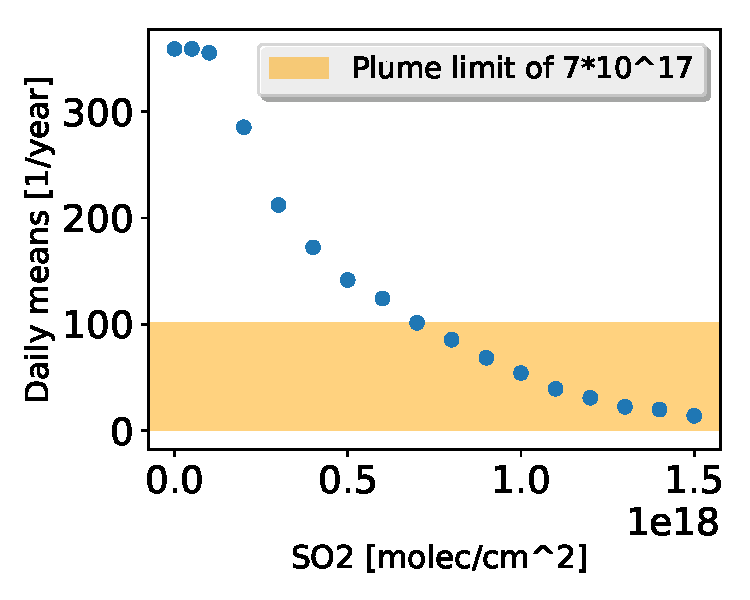
\includegraphics[width=0.7\linewidth]{Bilder/percentage_minSO2}
	\caption{The decrease of the amount of data above the plume limit as a function of the plume limit. The plume limits below the actual plume limit of 7$\cdot10^{17}$ are marked with a yellow shade.\textcolor{red}{noch dazu:In Prozent sieht das in der Tat schrecklich aus, relevant für eine Zeitreihenanalyse ist aber eher die (absolute) Anzahl der Tage mit (Multi-Scan-)Daten. Vielleicht als zweites Bild daneben?! }}
	\label{fig:percentageminso2}
\end{figure}

\section{Contamination problem\label{Chap:Cont}}
The conventional Evaluation is based on the assumption, that the reference is free of volcanic gases. This assumption was checked by using a volcanic gas free a high resolution solar atlas spectrum (see below) to evaluate the reference \cite{lubcke2014}; \cite{salerno2009novel}. In some reference spectra an amount of \ce{SO2}  different from zero is found. Thus we can conclude, that there are some references which contain a non-negligible amount of volcanic trace gases.
In rare (ca. 10\% of the data) scenarios, the
volcanic plume covers the whole scan region.
This could happen if for example the volcanic plume of the day before extends over the hole scan area as a consequence of windless conditions.
In consequence, the reference	is contaminated with volcanic trace gases. Thus, the gas amount is underestimated by the NOVAC-evaluation: In \Cref{fig:contaminated} we see an example from April 2011 (Tungurahua) where the reference region is contaminated by volcanic trace gases. The blue \ce{SO2} curve shows the calculations with the NOVAC-evaluation, but since there is still \ce{SO2} in the reference region, the assumption, that the \ce{SO2} amount could be set to zero in the reference region is wrong. The red curve shows the real \ce{SO2} curve, which lies significantly above the NOVAC -curve.\\
\\	
%
\\
\begin{figure}
	\centering
	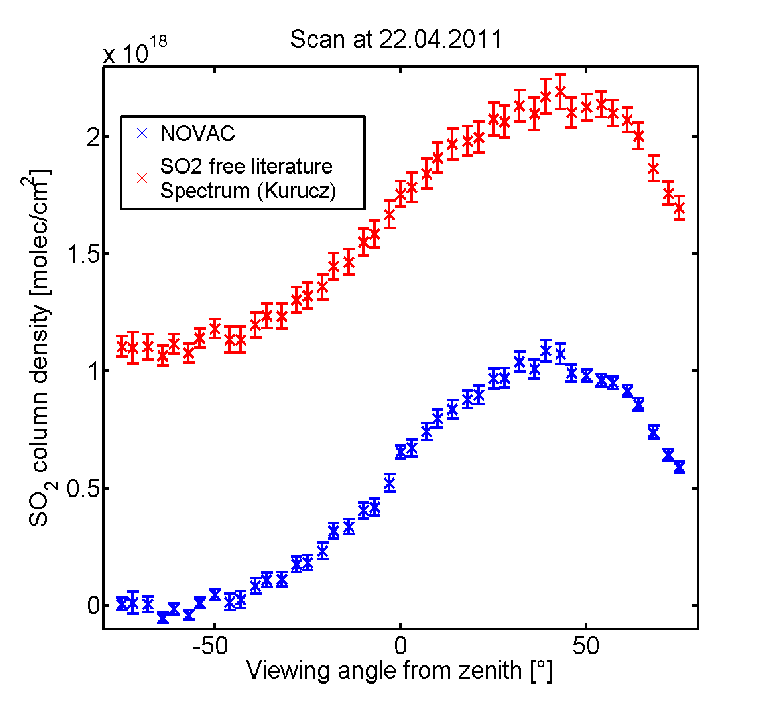
\includegraphics[width=0.7\linewidth]{Bilder/contaminated}
	\caption{Scan with a contaminated reference spectrum from April 2011. From \cite{WarnachSimon}}
	\label{fig:contaminated}
\end{figure}
If the reference region for any reason is
contaminated by volcanic trace gases, there are two possibilities: excluding the contaminated data from the evaluation or the reference spectrum has to be
replaced by a volcanic-gas-free reference. Alternative spectra are a
theoretical solar atlas spectrum or a volcanic-gas-free reference
spectrum recorded by the same instrument at another time.\\
A further possibility is to assume, that contamination only occurs for SO2, but not for BrO due to the smaller lifetimes of BrO, thus it is possible to use the Solar atlas spectrum for the \ce{SO2} evaluation, but the reference, recorded by the NOVAC-instrument at the same time for the BrO retrieval. Hereby the assumption, that BrO is not contaminated need to be proved. \\
%
\\
%
In the following we will discuss the two alternative reference spectra.
%
\subsection*{Evaluation using a Solar Atlas spectrum \label{kuruz}}
An alternative for choosing the region with the lowest column density as reference region is to use a theoretical high resolution solar atlas spectrum as reference \citep{chance2010improved}.
The use of a theoretical solar atlas spectrum as a reference which is completely volcanic-trace-gases-free was first proposed by \cite{salerno2009novel} and evolved by \citep{lubcke2014bro}.
The advantage of using a solar atlas spectrum as reference is, that we know that it is not affected by past or current volcanic gas emissions. Thus, it allows for a retrieval of the absolute trace gas SCDs in the volcanic gas plume. The disadvantage is, that using a solar atlas spectrum comes along with a drawback of precision: The spectral resolution of the theoretical solar atlas spectrum is much  higher than of the NOVAC instruments. Therefore the instrument functions would need to be perfectly modeled and added to the retrieval. This is not straight forward, because the instrumental line-shape varies over the wavelength region and is also mathmatically often not perfectly described by a simple approach like Gauss, lorents,..etc.\\ 
The reduction of precision is acceptable for the
\ce{SO2} retrieval but not suitable for a \ce{BrO} retrieval because then most data would be below the detection limit.\\
%
\\
%
Possible contaminations can be checked
by a theoretical solar atlas spectrum to evaluate the \ce{SO2} amount in the reference.\\

%
\subsection*{Evaluation using a spectrum of the same instrument}
An alternative reference spectrum could be a volcanic-gas-free reference
spectrum recorded by the same instrument at a different time. When using such a reference several problems occur:\\
As described in \Cref{NOVAC} the instruments used in NOVAC do not include features like temperature stabilization. Due to that the measurements are not independent of external parameters. 
So we need to choose a reference recorded at similar conditions with respect to meteorology and	radiation as well as in the temporal proximity due to instrumental changes with time and ambient conditions. Ideally the external conditions should be equal to the conditions at the time when the plume was recorded.\\
\\
%
When performing the evaluation with the Solar Atlas Spectrum as reference, finding the instrument function occur to be a central challenge. If the instrument function for the solar atlas spectrum is found the functions is typically used for a few years This could lead to higher errors due to an gradual worse matching instrument function.
Using the reference of the same instrument but recorded at another day, leads also to problems caused by different instrument functions, but compared to the calculated instrument function used for the evaluation with the solar atlas spectrum those differences in the instrument function could be smaller.
\\
In this work we combine both options in order to
achieve both, enhanced accuracy but still maximum possible precision of
the \ce{SO2} and \ce{BrO} retrievals. So we use the solar atlas spectrum to check for 
contamination and a reference spectrum recorded in temporal proximity by the same instrument as reference.\\
\\
If contamination occurs it is possible to choose a new reference from a list of gas free alternative references. In theory, for ideal instruments all references should lead to
	the same results for the gas retrievals. But instruments are imperfect (see Chapter
	4) thus the reference need to be chosen carefully in order to ensure reliable results.\\
%
\\
As discussed above it might occur, that the reference is contaminated for example by the plume of the day before.
%\textcolor{green}{das verstehe ich jetzt nicht - ich meine wenn wir jetzt das solar atlas spectrum nehmen ueberschaetzen wir ja , weil wir fahne von gestern und heute als eine einzige Fahne zusammen addieren...
%	unterschaetzung haben wir wenn der bei zum beispiel kleiner windgeschwindigkeit -> breite fahne das instrument in keiner richtung fahnen freien himmel sieht - oder bei hoher windgeschwindigkeit und instrument nah am berg die fahne so runtergedreuckt wird das das instrument in der fahne steht..: Florian : @ Nicole zur Überschätzung: wenn wir annehmen, dass die alte, bodennahe Fahne überall die gleiche Dicke hat und die neue Fahne eher im Zenit steht, dann ist der Anteil der alten Fahne zum neuen Gesamtsignal kleiner als der alten Fahne zum neuen Referenzsignal. D.h. Überschätzung ja, aber weniger als simple Addition.} 
If that happens, we underestimate the gas amount by using a contaminated reference. But another possibility is, that the plume itself is also contaminated. This might be the case if the volcanic gas of the volcano is not taken away by the wind, but accumulates at the instrument. If this is the case, using an other reference would lead to an overestimation of the column density of gases. With the data retrieved by the NOVAC instruments it is very difficult to discover whether the plume is contaminated or not. \\
\Cref{fig:contaminationdependencyso2} shows the strength of contamination as function of the mean \ce{SO2} amount of the day before. The strength of contamination is  measured as the difference between the evaluation for \ce{SO2} with a contaminated reference recorded at the same time as the plume spectrum was recorded and using a gas free reference. The data where fitted with a linear function. The left plot shows data from the Tungurahua volcano. In the right plot the data of Nevado Del Ruiz are visualized. Even though both plots show a slight increase of contamination strength with the mean amount of \ce{SO2} of the day before, the increase is not significant.\\
\textcolor{red}{hier waere es gut noch andere parameter zu testen - wie in Luebcke et al, zum beispile als funktion von Wind geschwindigkeit,..   Für NdR kann ich die Meteorologischen Daten ab 2014 beisteuern.}
\\
However this thesis is build on the assumption, that the plume is free of additional contamination \textcolor{yellow}{Nicole hat hier noch fragen, was ?}. In the following we discuss how to automatically determine an optimal reference from another scan.
\begin{figure}
	\subfigure{
	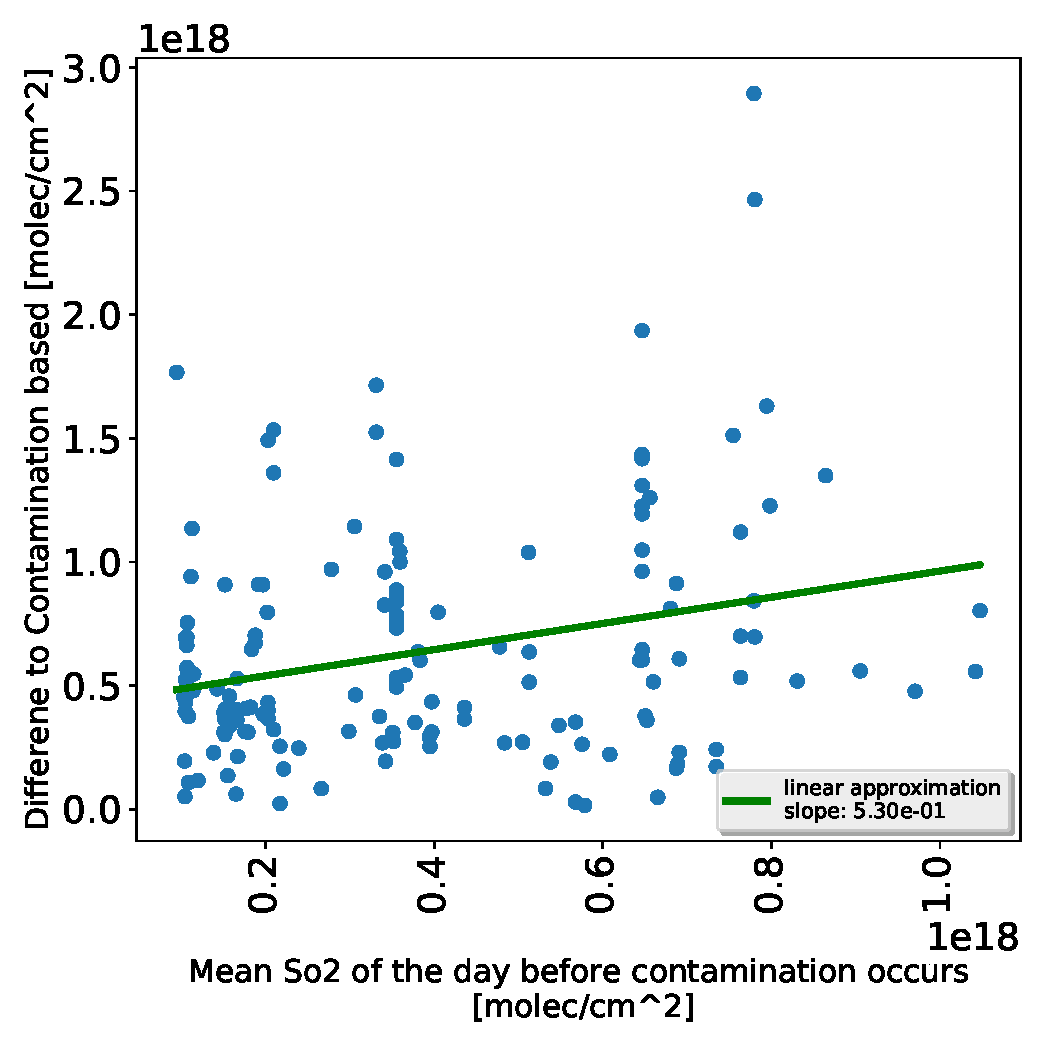
\includegraphics[width=0.5\linewidth]{Bilder/contaminationdependency_so2}}
\subfigure{
	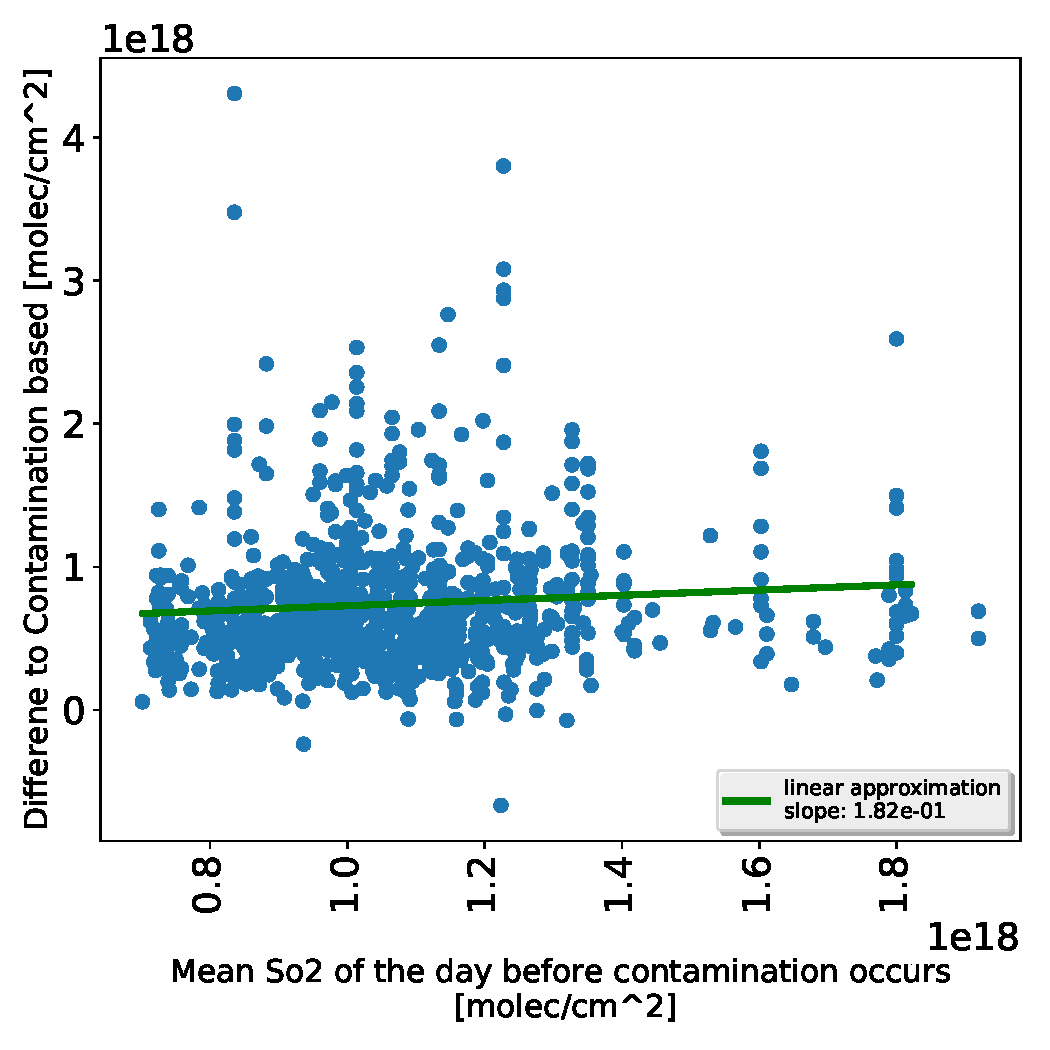
\includegraphics[width=0.5\linewidth]{Bilder/contaminationdependency_so2_Nevad}}
	\caption{The strength of contamination as function of the mean \ce{SO2} amount of the day before. The strength of contamination is defined as the difference in \ce{SO2} SCD  when evaluation with an alternative reference, or neglect the contamination. Left: data from Tungurahua. Right: data from Nevado Del Ruiz. \textcolor{red}{Wie wurde mean \ce{SO2} bestimmt? Wie sieht es bei max \ce{SO2} aus? (Und eigentlich müsse man ja eher die \ce{SO2} Emissionen anschauen. Die wir aber nicht (so einfach) kennen.)}}
	\label{fig:contaminationdependencyso2}
\end{figure}
	\chapter{\ce{BrO}  Evaluation and its limitations}
	This chapter discusses the evaluation of \ce{BrO}  by spectroscopic instruments of NOVAC.\\
	The evaluation of the data from NOVAC is parted into the evaluation of SO2 and the evaluation of BrO. While the retrieving of SO2 is relatively easy due to the high amount of SO2  (magnitude of \ce{SO2} at Tungurahua $\approx 1e^{18}$), the BrO evaluation is much more problematic (as it can be seen in \Cref{fig:plumeref}). The magnitude of BrO SCD is around $\approx 1e^{14}$. 
	This results in a larger uncertainty of the \ce{BrO}  SCD. Most of te \ce{BrO}  data are below the detection limit of \ce{BrO}$_{err}$/BrO$_{value}$<1/4. In comparison SCDs of \ce{SO2}  are in almost all cases (99.5\% of the data) above the detection limit. 
	Choosing a different reference than the reference meausred at the same time as the plume results in 99\% of all data in an increasing absolut error. 
	%
	Thus an \ce{BrO} error which is smaller than the "Same Time Error" is often not  possible to retrieve. However, due to the large uncertainty of BrO relative to So2 this thesis will concentrate on BrO analysis. Thus, the reference is chosen with respect to the BrO error to maximise the quality of the BrO/SO2 ratio. The amount of gas free alternative references is around 1500 per year. To make the best choice it is necessary to examine the conditions which influence the BrO retrieval.
	\\
	Every spectrum is measured under certain conditions. These conditions in general are not the same when measuring the plume and the reference.
	References where the surrounding conditions e.g temperature or cloudiness are equivalent with the surrounding conditions of the  plume measurement lead to a small error.
	In the following, we will take a closer look at the dependency of the \ce{BrO} error on external parameters. 
	%
	\subsubsection*{Data used for the analysis}
	For this analysis every plume reference pair of the observed time span is used. Thus for 1000 recorded "multi add" spectra results in $1000^2$ plume reference pairs and their the corresponding differences in the external parameter and their associated \ce{BrO} error.

	\section{\ce{BrO} error dependence on external parameters \label{Chap:BROErr}}
	%HOW IS THE ERROR CALCULATED AND WHY AND DETECTION LIMIT (PLATT \& STUTZ)
	The measurement and evaluation depends on the surrounding conditions like temperature or cloudiness \citep{lubcke2014optical}\\
	As a result the surrounding conditions need to be taken into account if choosing a new reference.\\
	The better the surrounding conditions of the time where the reference is measured coincide with the conditions of the time when the plume is measured. The lower the time difference, the lower the expected BrO error.  \\
	\\

	The surrounding conditions that are considered in this thesis are: 
	\begin{itemize}
		\item Temporal difference between measuring the plume and the reference.
		\item Temperature, 
		\item Colorindex, 
		\item Exposure time, 
		\item Elevation angle, 
		\item Daytime 	
	\end{itemize}
	The analysis of these external parameter is done for spectra recorded at Tungurahua and Nevado Del Ruiz (see \cref{Tung}). 
	
	
	
	
	\subsection{Temporal difference}
	\begin{figure}
		\centering
		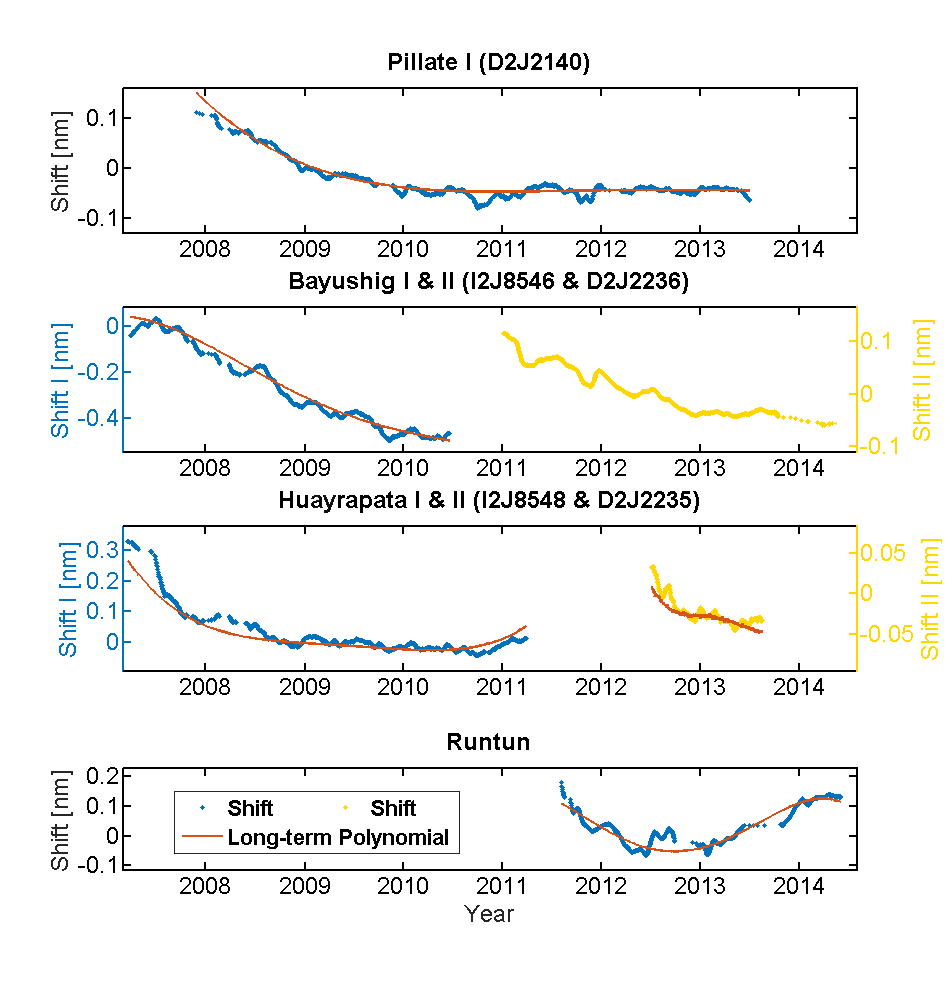
\includegraphics[width=1\linewidth]{Bilder/Simon/Bilder_Tung/Drift_Komplett_NEW}
		\caption{Wavelength shift over the time. The shift is shown for six NOVAC- instruments from Tungurahua. The red and yellow dots show the running mean about 20 days. Red line indicates a temperature independent long term polynomial. From \cite{WarnachSimon}}
		\label{fig:driftkomplettnew}
	\end{figure}
	%
	\begin{figure}
		\subfigure[]{
			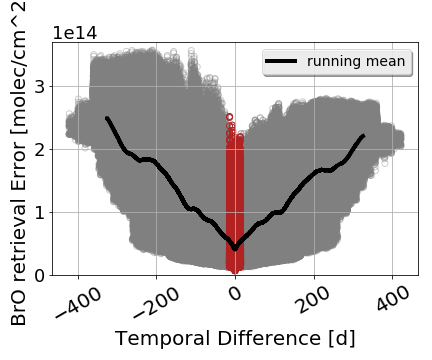
\includegraphics[width=0.5\linewidth]{Bilder/Datum}}
		\subfigure[]{
			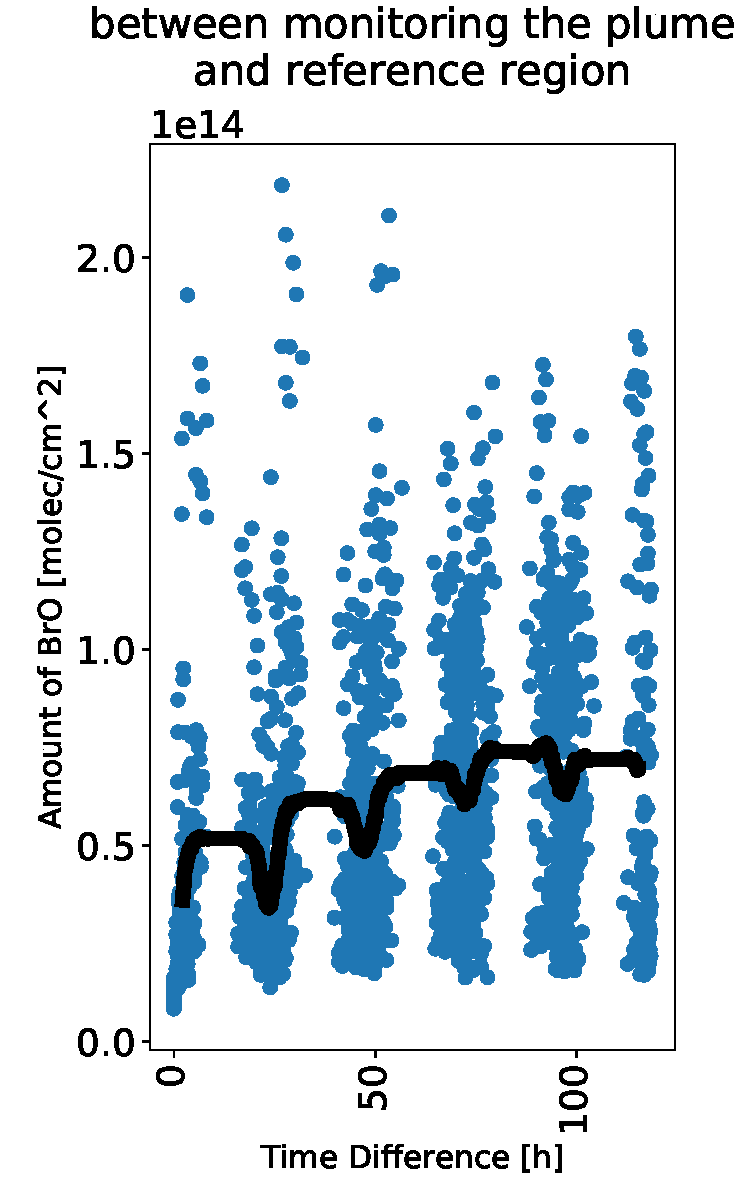
\includegraphics[width=0.5\linewidth]{Bilder/Datum_100h}}
		
		\caption{The \ce{BrO}  error as a function of the temporal difference shown for the Pillate instrument from Tungurahua (2008-2009). (a) Temporal differences up to 400 days are shown. (b) Temporal differences below 120h; periodical \ce{BrO}  error evolution indicates the impact of the daytime}
		\label{fig:dat}
	\end{figure}
	Due to instrument drifts the fit quality decreases with the time difference between recording the plume and the reference. This could be a result of a wavelength shift over time which was observed by \cite{WarnachSimon}. \cite{WarnachSimon} suggested that the drift is caused by a hysteresis effect. \Cref{fig:driftkomplettnew} show the wavelength shift as a function of the time for six NOVAC instruments located at Tungurahua in the time between 2008 to 2014. For the analysis in this thesis data of Tungurahua between 2008 to the mid of 2009 are used. \Cref{fig:driftkomplettnew} shows a rather steep drift in this time interval. \cite{WarnachSimon} observed a decrease of the shift after initial negative drift after the first 2 years at Pillate. Thus, it could be that the temporal difference could become less important for old instruments. For the following discussions date of Pillate from 2008 to 2009 are used.\\
	%
	When using reference and plume spectra of the same time, these effects are cut out since the shift is equal for the plume and reference spectrum. For increasing temporal different between reference and plume measurement time the fit quality decreases and thus the \ce{BrO} error increases.\\
	In \Cref{fig:dat} the \ce{BrO} error as a function of the time difference between recording the plume and the reference is shown. The running mean is drawn with a black line. \\
	In \Cref{fig:dat} (a) it can be seen that a large temporal difference result in an increase of \ce{BrO} error of more than 600\%. \ce{BrO} errors of such magnitudes are too large for our purposes therefore it is useful to define a maximal temporal difference.\\
	The maximal temporal difference should be large enough to ensure an amount of references which is large enough to be able to pick a reference with similar conditions, but the maximal temporal difference should be small enough to prevent to large BrO errors due to long term shifts.\\
	To evaluate the maximal time difference, for which we still get reliable results for all possible reference-plume pairs the corresponding BrO error was calculated. With this data for all plume spectra we are able to find the associated reference where the BrO error is minimal. In \Cref{fig:Hist} a histogram is plotted with the probability of picking the best reference as a function of the time difference. Obviously the best results are obtained in cases where the day of measuring the reference is the same day as measuring the reference. That means, if the time difference is smaller than one day. A gauss fit was used to fit the data of the histogram We allow all time differences which are in two sigma area. Thus the maximal time difference is 14 days\\
	%
	\begin{figure}
\centering
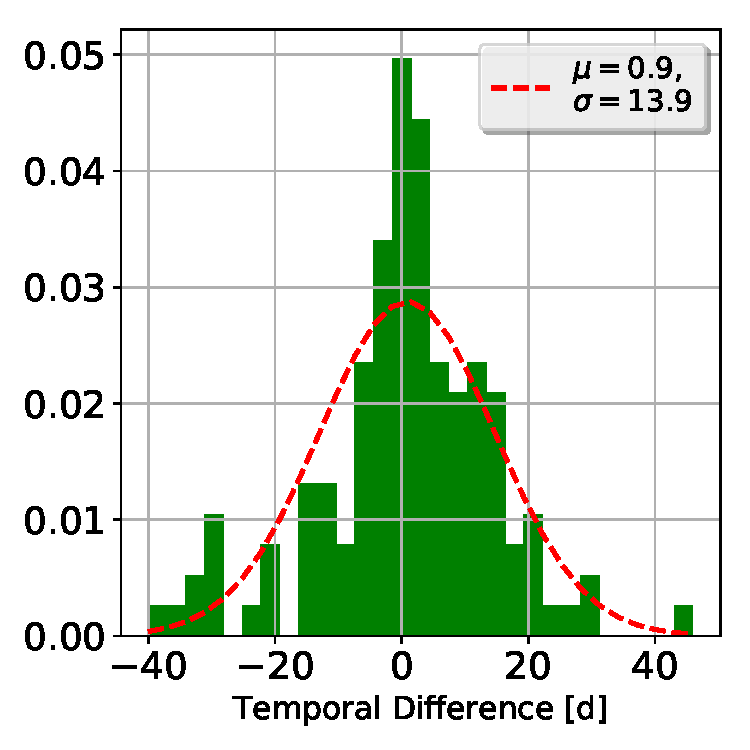
\includegraphics[width=0.7\linewidth]{Bilder/Hist}
\caption{Histogram showing the frequency of getting the best reference as function of the temporal difference between plume and reference measuring.}
\label{fig:Hist}
\end{figure}

	 \Cref{fig:dat} (b) shows the evolution of the \ce{BrO} error for a maximal temporal difference of 120 hours. It is only possible to record data during daytime. This couses the lack of data at some temporal differences. A periodic decrease of the \ce{BrO}  error can be seen. This is a result of a decrease of the \ce{BrO}  error when the surrounding conditions coincidence. In this case the daytime coincidence couses the \ce{BrO}  error to decrease. For further discussion of the daytime see \Cref{chap:daytime}.\\
	%
	By restricting the temporal difference to 14 days the amount of possible gas free references decreases on an average of 195 alternative references per contaminated plume (see \cref{Tab:refstime}). Whereas none of the plumes do not have alternative references. The minimum amount of references is 8.\\
	If a continuously evaluation is required, this means the spectra are evaluated directly after the recording, the number of suitable gas free references halves since only references recorded before the plume are available.\\
	For the following analysis of external parameters all temporal differences are below 14 days.
	%
	\begin{figure}		
		\subfigure[]{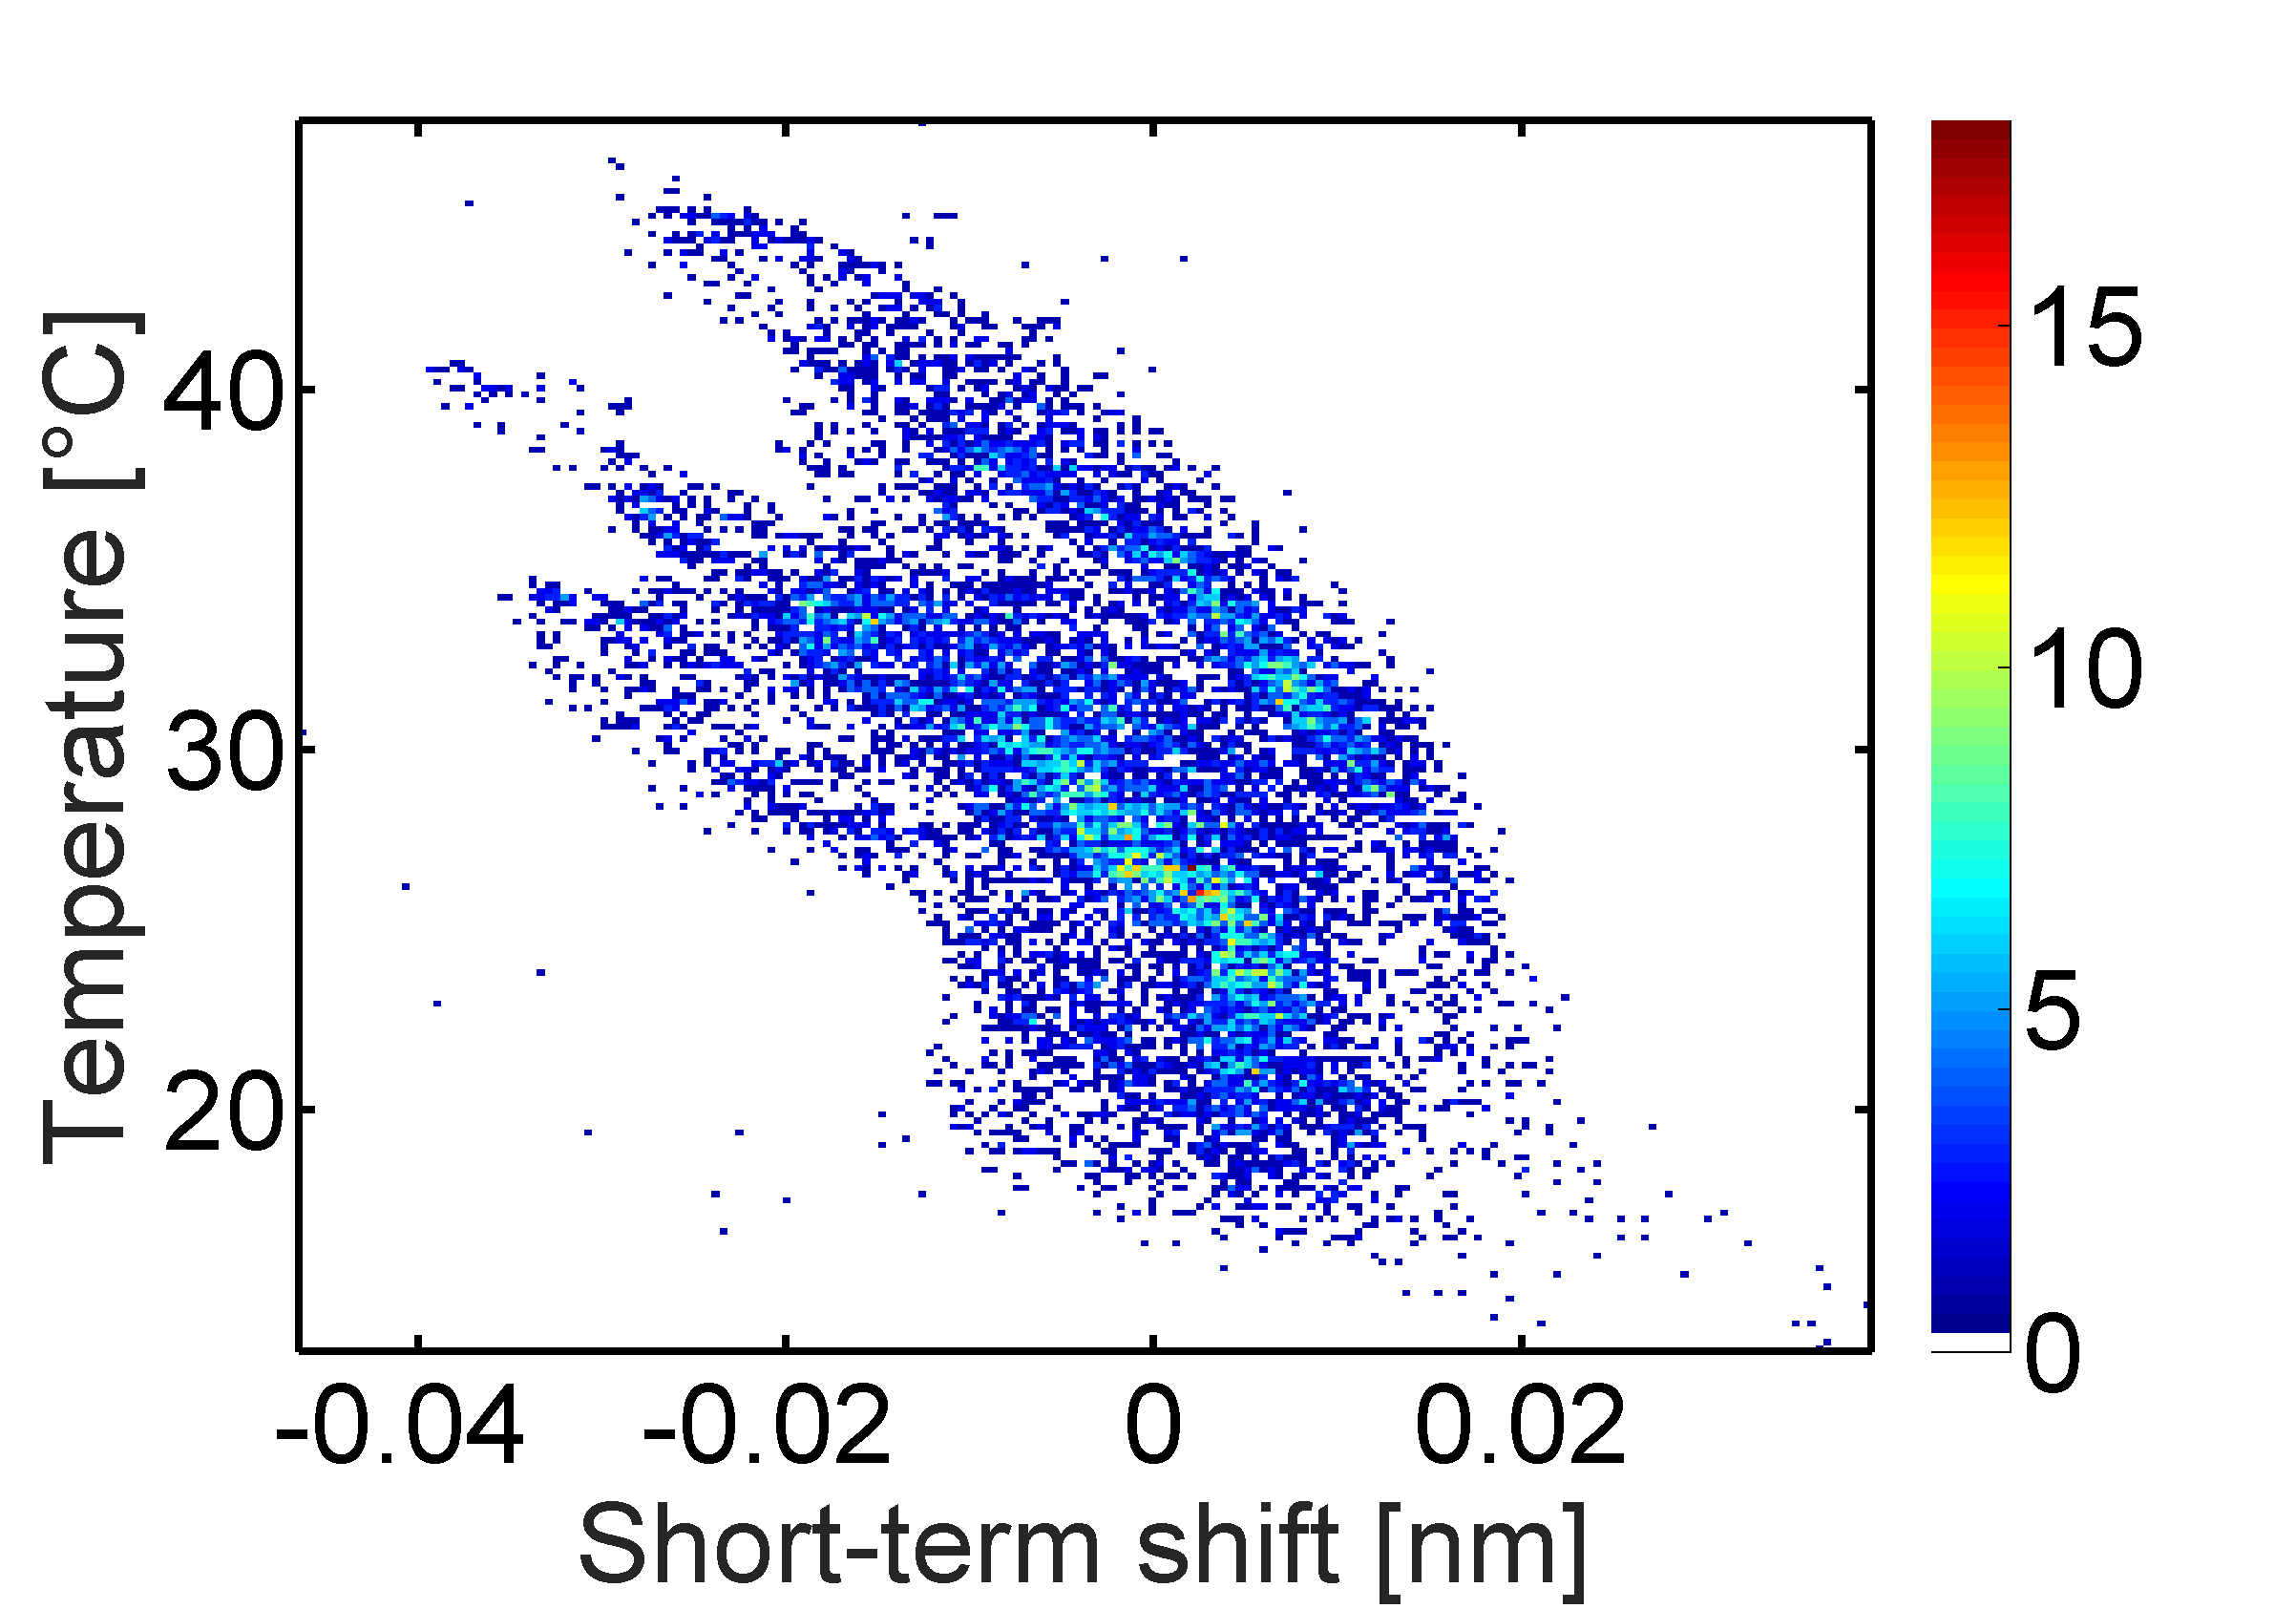
\includegraphics[width=0.49\textwidth]{Bilder/Simon/Bilder_Tung/D2J2140_Before}}
		\subfigure[]{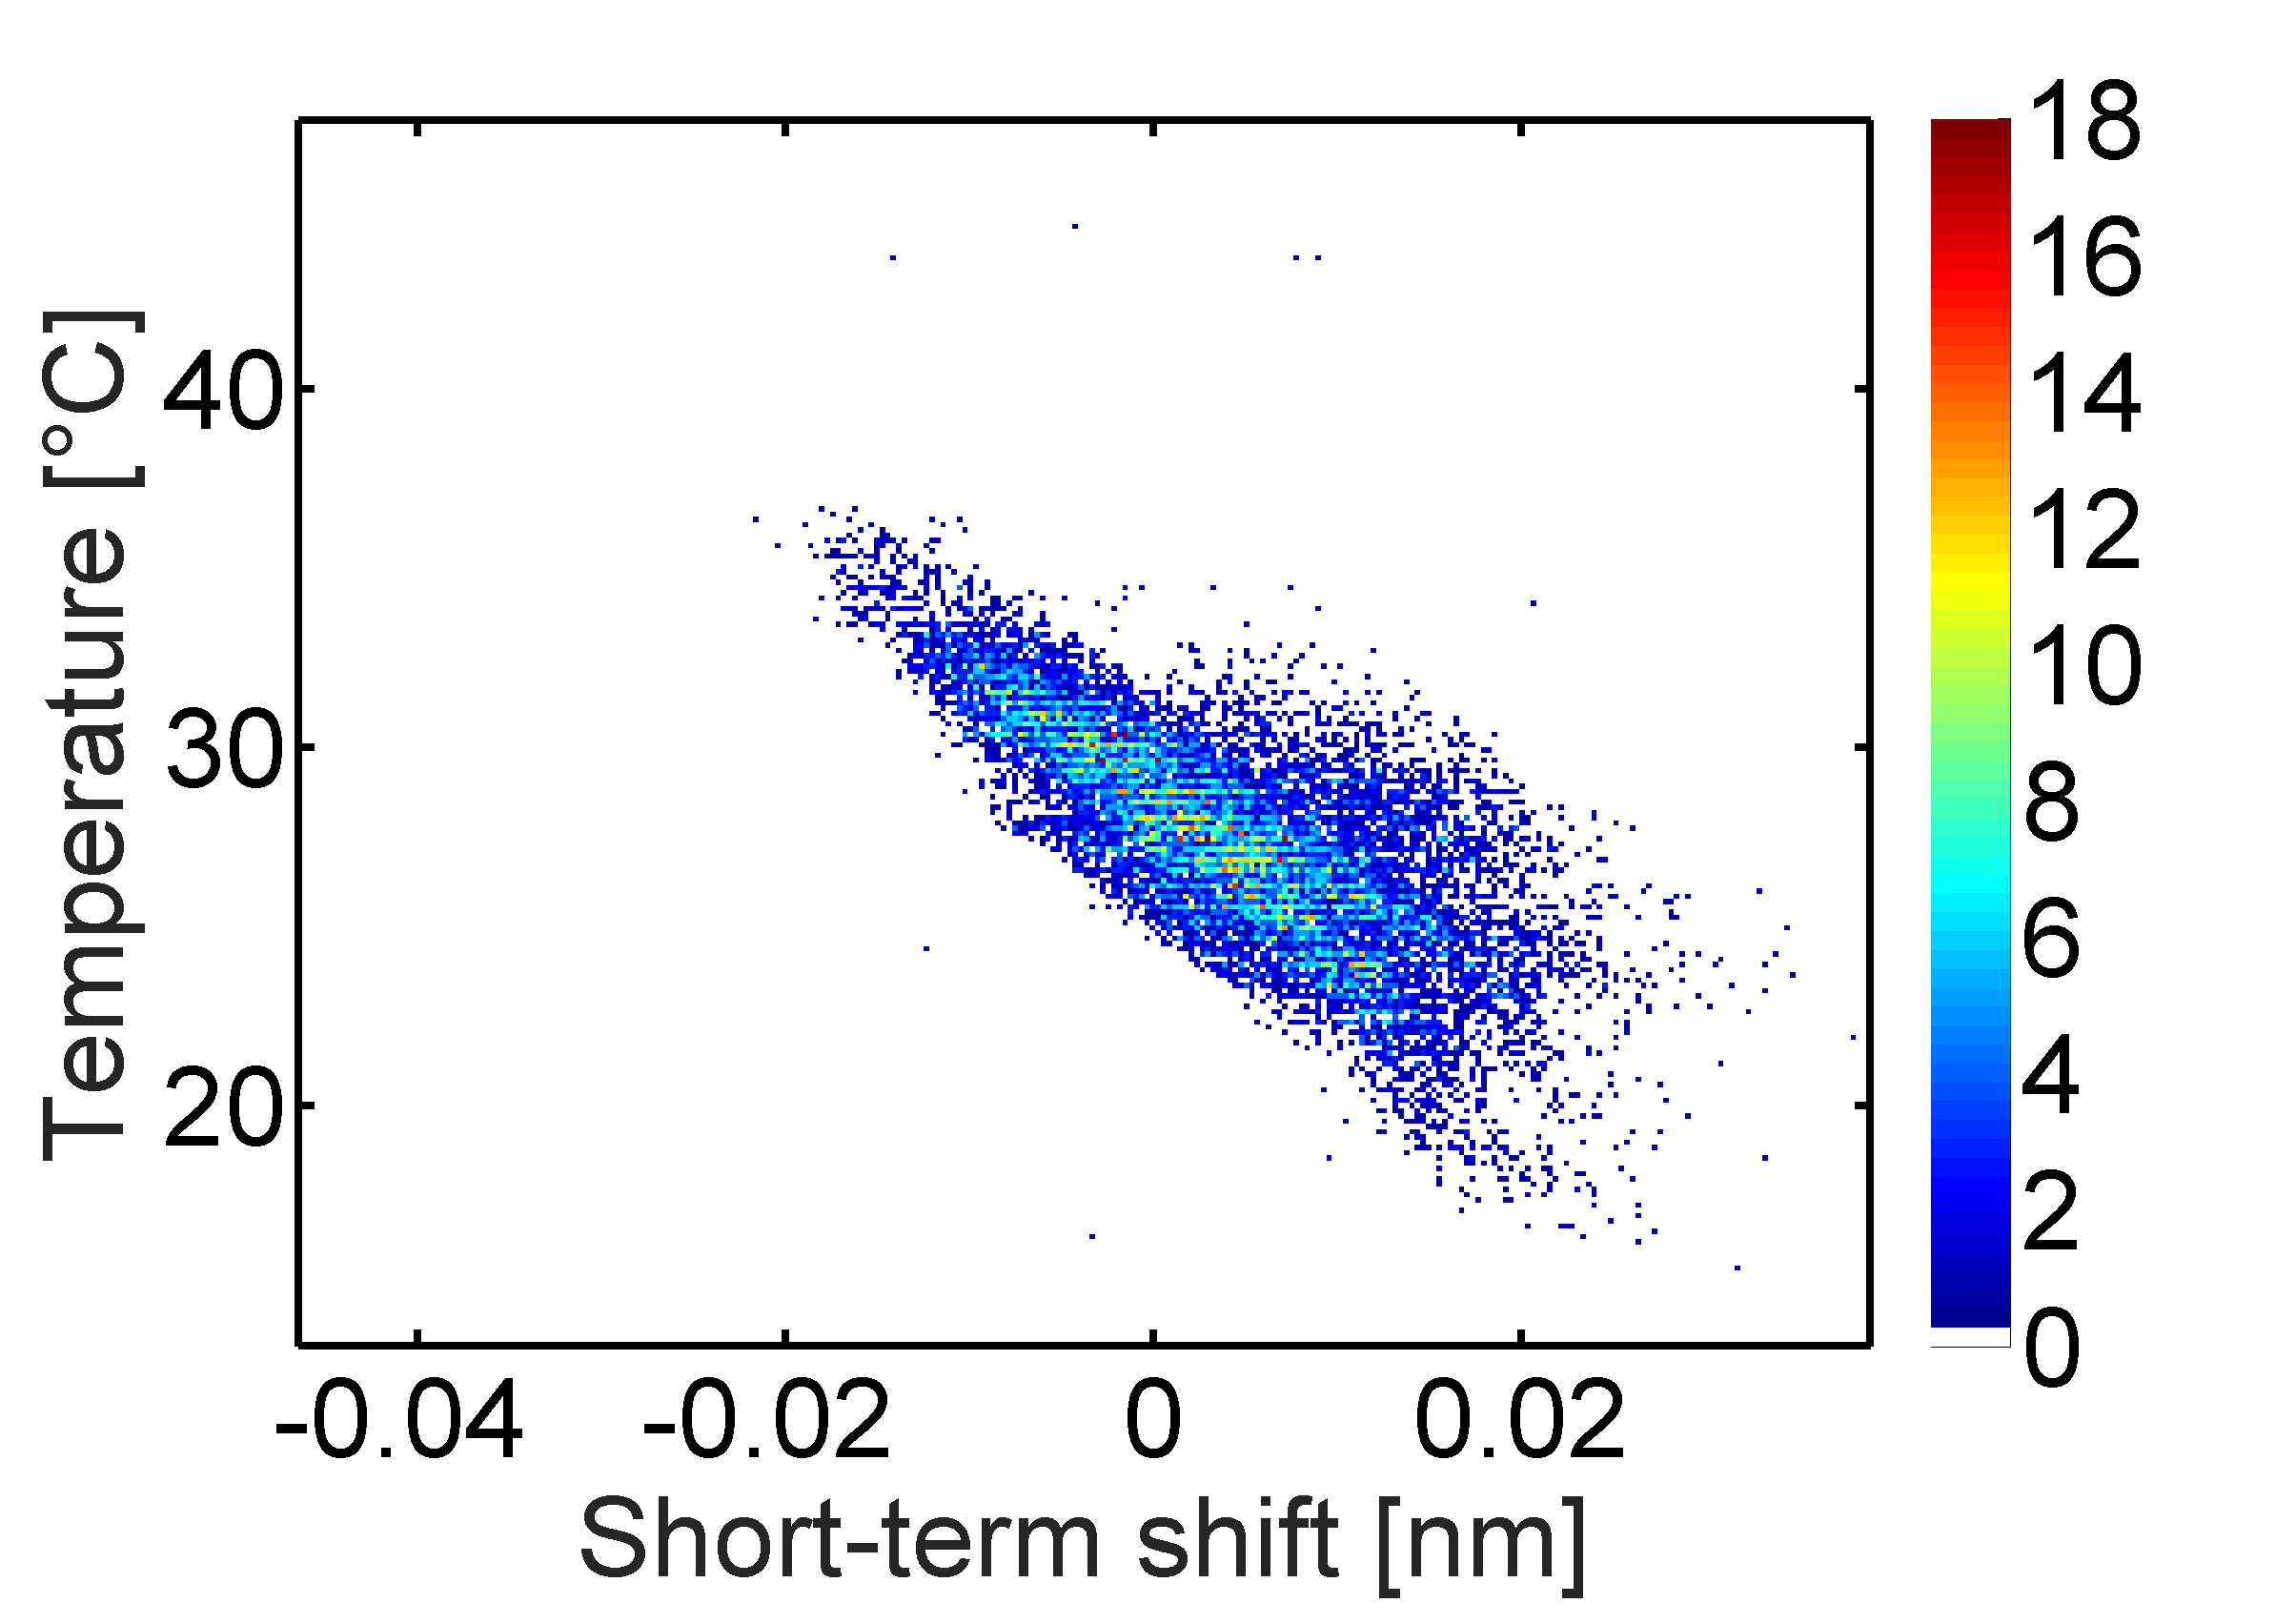
\includegraphics[width=0.49\textwidth]{Bilder/Simon/Bilder_Tung/D2J2140_After}}
		\caption{Short Term wavelength as a function of the instrument temperature for Pillate 1. (a) initial period  prior to January 2010 (b) after 2010. From \cite{WarnachSimon}}
		\label{fig:shorttermshift}
	\end{figure}

	\begin{table}[h]
		\begin{tabular}{|p{2cm}|p{2cm}|p{2cm}|p{2cm}|p{2cm}|p{2cm}|}
			%	\toprule
			Instrument	&D2J2140\_0&I2J8546\_0& I2J8548\_0&D2J2200\_0&D2J2201\_0\\
			\toprule
			Mean&84.6 $\equiv$ 100\%&163.7 $\equiv$ 100\%&217.1 $\equiv$ 100\%&284.0 $\equiv$ 100\%&225.6 $\equiv$ 100\%\\
			\midrule
			Std&
			35.8 $\equiv$ 100\%&
			29.9 $\equiv$ 100\%&
			64.8 $\equiv$ 100\%&
			69.5 $\equiv$ 100\%&
			41.2 $\equiv$ 100\%\\
			\midrule
			Min&
			8 $\equiv$ 100\%&
			113 $\equiv$ 100\%&
			97 $\equiv$ 100\%&
			64 $\equiv$ 100\% &
			63 $\equiv$ 100\%\\
			\midrule
			Max&
			169 $\equiv$ 100\%&
			214 $\equiv$ 100\%
			&399 $\equiv$ 100\%
			&433  $\equiv$ 100\%
			&297 $\equiv$ 100\% \\
			\bottomrule
		\end{tabular}
	\caption{Amount of possible references while restricting the time span between plume and reference to two weeks.}
	\label{Tab:refstime}
	\end{table}	

	Furthermore it can be seen that the evolution of the \ce{BrO}  error with the temporal difference is symmetric around zero, thus it is not necessary to distinguish between positive or negative temporal differences.\\

	
	\subsection{Temperature}
	\begin{figure}
		\subfigure[D2J2140\_0]{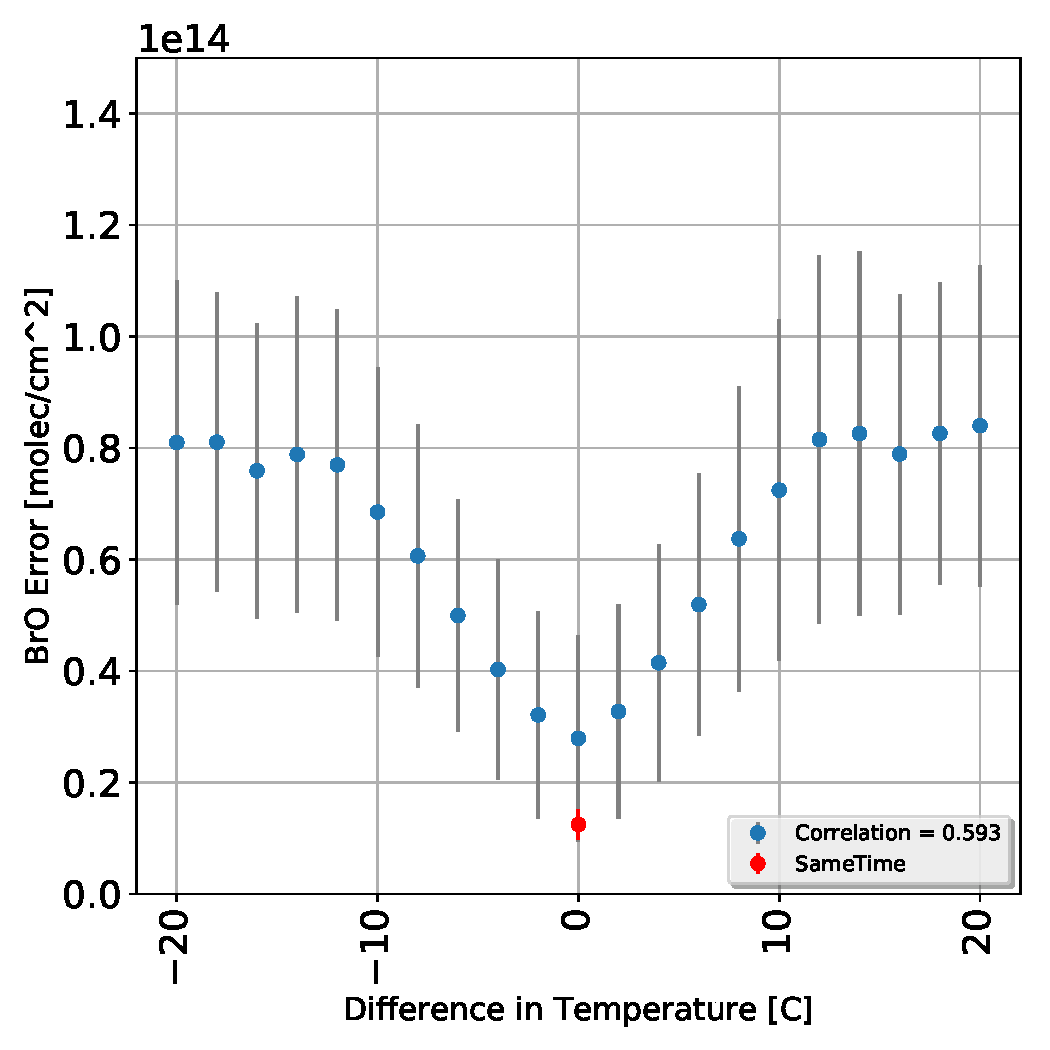
\includegraphics[width=0.3\linewidth]{Bilder/DEpendencoOfBrOErrorOnVariables_absolutedep/D2J2140_0BrOERR_DiffTemp_Tungu}}
		\subfigure[I2J8546\_0]{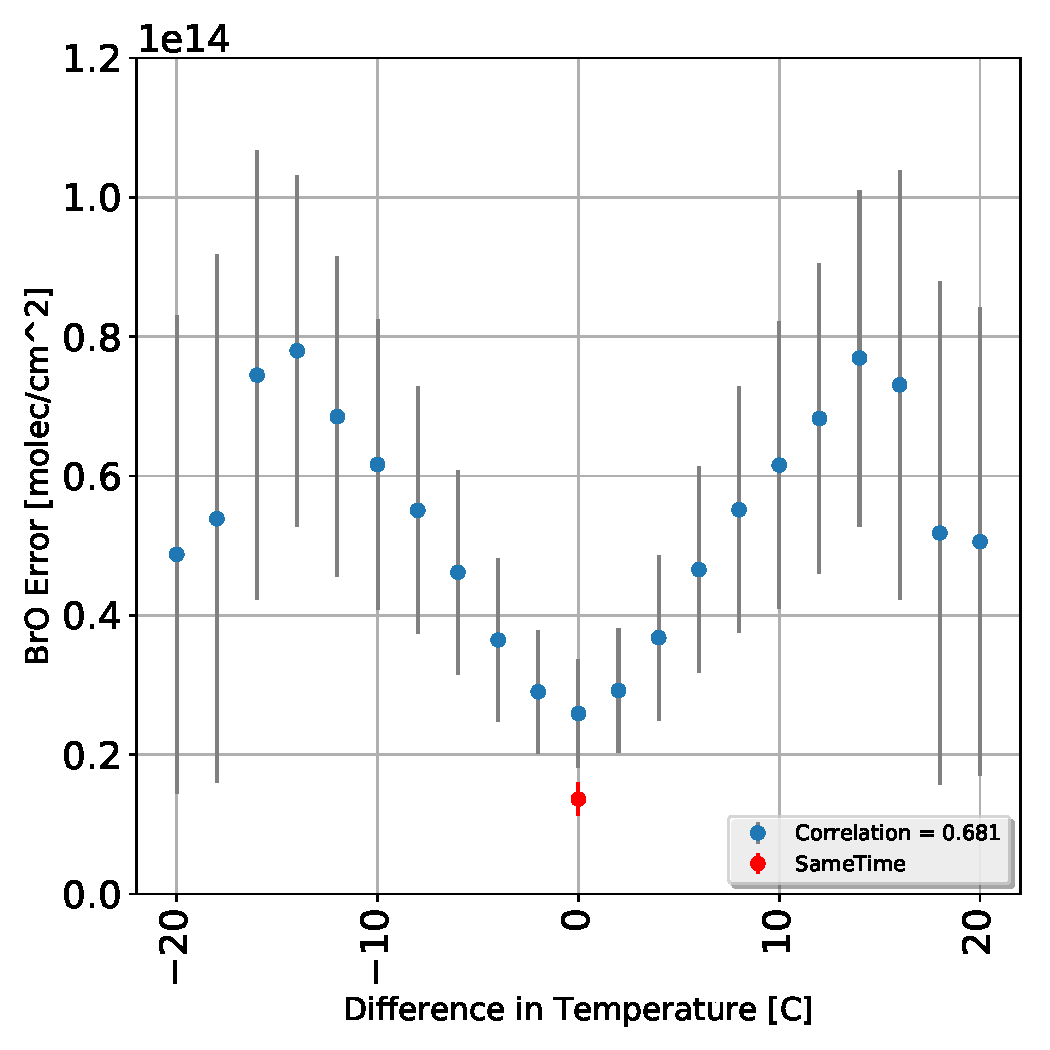
\includegraphics[width=0.3\linewidth]{Bilder/DEpendencoOfBrOErrorOnVariables_absolutedep/I2J8546_0BrOERR_DiffTemp_Tungu}}
		\subfigure[I2J8548\_0]{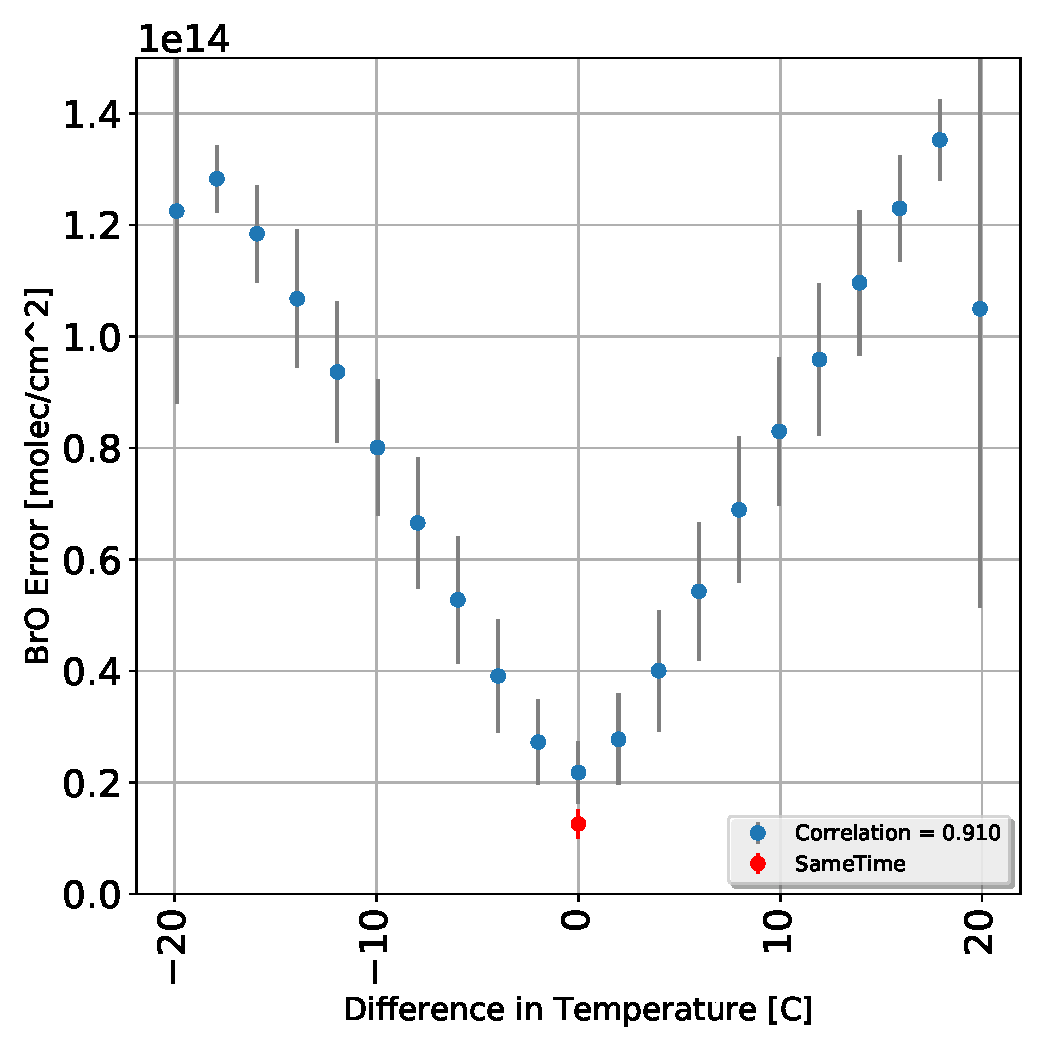
\includegraphics[width=0.3\linewidth]{Bilder/DEpendencoOfBrOErrorOnVariables_absolutedep/I2J8548_0BrOERR_DiffTemp_Tungu}}
		\centering
		\subfigure[D2J2200\_0]{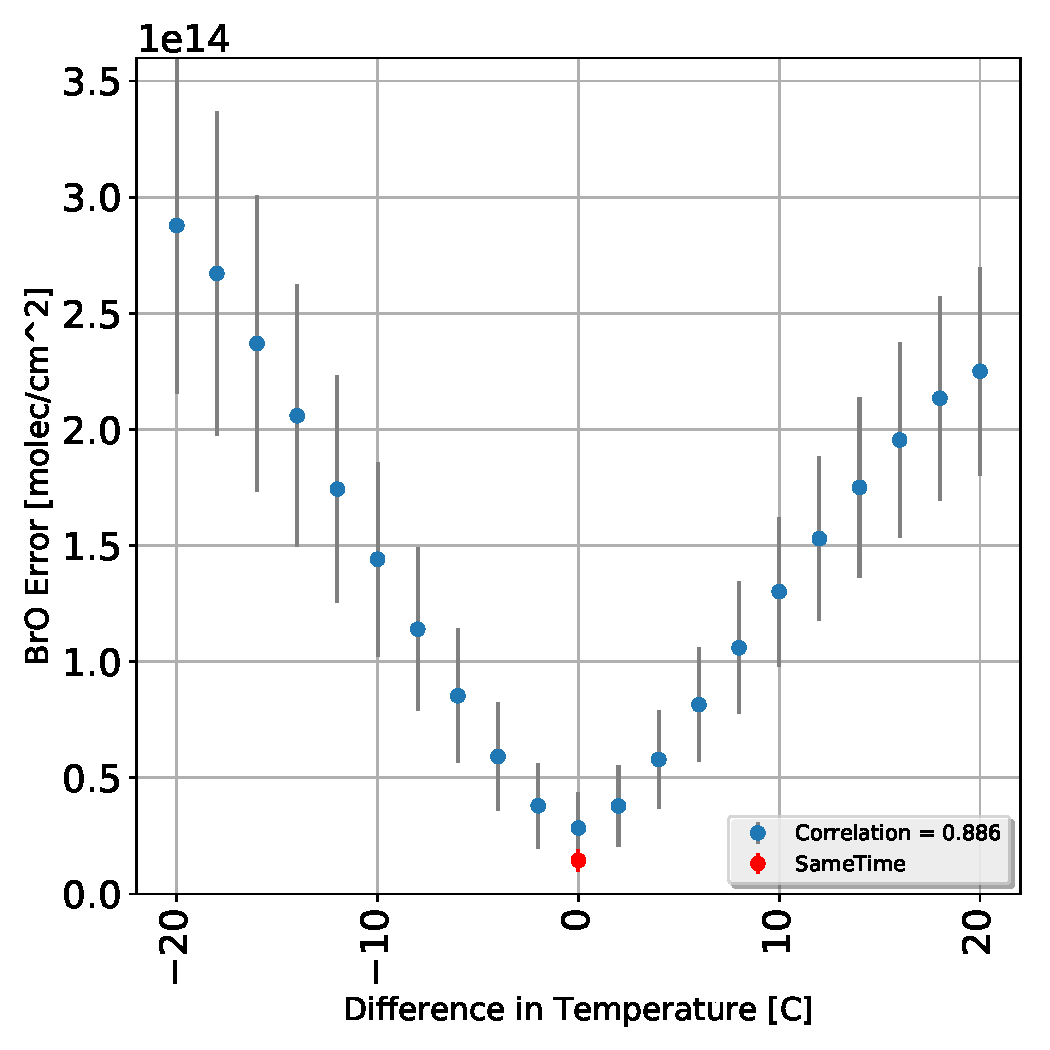
\includegraphics[width=0.3\linewidth]{Bilder/DEpendencoOfBrOErrorOnVariables_absolutedep/D2J2200_0BrOERR_DiffTemp_Nevad}}
		\subfigure[D2J2201\_0]{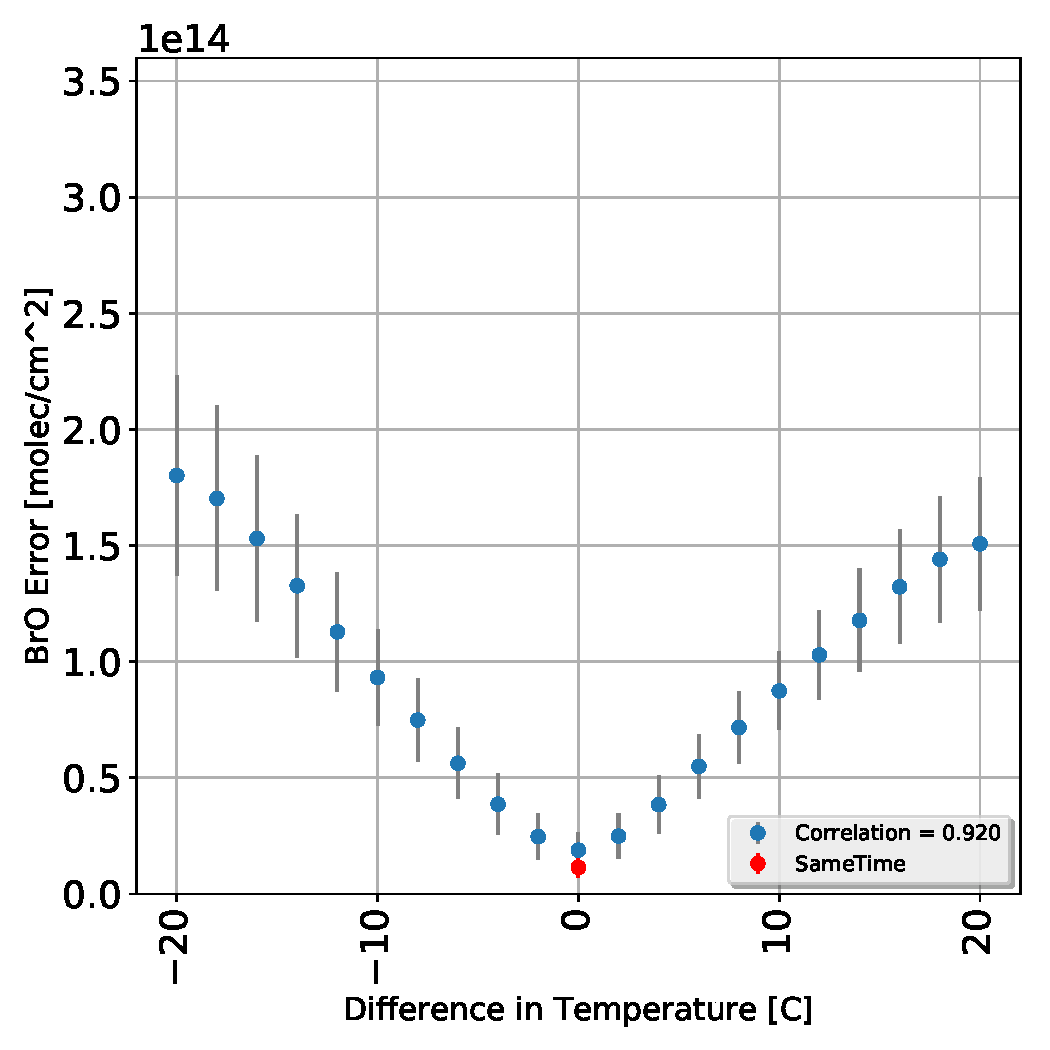
\includegraphics[width=0.3\linewidth]{Bilder/DEpendencoOfBrOErrorOnVariables_absolutedep/D2J2201_0BrOERR_DiffTemp_Nevad}}
		\caption{The \ce{BrO}  measurement error as a function of the difference of temperature between measuring the reference and the plume are shown. (a)-(c) show the data for the instruments at Tungurahua, (d)+(e) at Nevado Del Ruiz. To evaluate the plume spectra all reference spectra with a temporal distance of no longer than two weeks are used. A increase of the \ce{BrO} error with the distance in temperature is observable.}
		\label{fig:difftemp}
	\end{figure}
	The instrument design of the NOVAC instruments compromise between accuracy and longetivity as explained in \Cref{NOVAC}. In particular there are no internal thermal stabilizations installed as an attempt to reduce the instruments power consumption. This can influence the recorded spectra.\\	
	Each pixel of the spectrometer, which is used for the DOAS experiment, collects photons of a certain wavelength range.\\
	The calibration for the wavelength to pixel mapping (WMP) is commonly done with a Mercury lamp or by the comparison with the high defined Kuruz spectrum.
	As the WMP depends on the optical alignment of the spectrometer, which itself depends on the temperature, it is not constant.
	Changes in the spectrometers temperature can cause changes in the instrument line function and shifts in the WMP (\citep{pinardi2007influence}). 
	Moreover, \cite{WarnachSimon} show that, short term shifts are related to the instrument temperature (see \Cref{fig:shorttermshift}).\\
	The above discussed temperature dependence of the WMP causes a reduction of the fitquality with increasing instrument temperature difference between plume and reference. Thus the \ce{BrO} error increases as well with the temperature difference. To quantify the \ce{BrO} error dependency on the temperature all plume spectra of Tungurahua from August 2008 to August 2009 (Nevado del Ruiz from end of 2009 to the end of 2011) are evaluated  with respect to all plume spectra of the same time period. 
	The \ce{BrO} error as function of the temperature difference can be seen in \Cref{fig:difftemp}. The blue dots shows the mean \ce{BrO} error at the specific temperature difference, the standard deviation is illustrated with gray bars.\\
	The mean \ce{BrO}  deviation for the sametime evaluation is additionally added with a red point.


	\begin{table}[h]
		\begin{tabular}{|p{2cm}|p{2cm}|p{2cm}|p{2cm}|p{2cm}|p{2cm}|}
			%	\toprule
		Instrument	&D2J2140\_0&I2J8546\_0& I2J8548\_0&D2J2200\_0&D2J2201\_0\\
			\toprule
			Slope&4.10e+12 &3.93e+12 &6.50e+12 &1.24e+13&8.17e+12 \\
			\midrule
			Correlation
			& 
			0.593& 
			0.681& 
			0.910& 
			0.886& 
			0.920\\
			\midrule
			Zero point&2.58e+13&2.23e+13&1.60e+13& 1.38e+13& 9.07e+12\\
			\midrule
			$\Delta T_{2}$&6.3&5.7&2.5&1.1&1.1\\
			\bottomrule
		\end{tabular}
		\label{tab:tempe}
	\end{table}
	When looking at all discussed external parameters, temperature has  the strongest impact on the \ce{BrO} error due to the strong impact on the WMP.



	\begin{table}
	\begin{tabular}{|p{2cm}|p{2cm}|p{2cm}|p{2cm}|p{2cm}|p{2cm}|}
		%	\toprule
		Instrument	&D2J2140\_0&I2J8546\_0& I2J8548\_0&D2J2200\_0&D2J2201\_0\\
		\toprule
		Mean&
		39.6/46,8\%&
		119.3/72,9\%
		&158.2/72,9\%
		&233.6/82,3\%
		&151.6/67,2\%\\
		\midrule
		Std&
		24.66/68,9\%&
		50.4/168,6\%&
		75.97/117,2\%&
		84.5/121,6\%&
		72.6/176,2\%\\
		\midrule
		Min&
		1/12,5\%
		&8/7,1\%&
		12/12,4\%&
		3/4,7\% &
		6/9,5\%\\
		\midrule
		Max
		&
		130	/76,9\%&
		213	/99,5\%&
		386/96,7\%&
		414	/95,6\% &
		296	/99,7\%\\
		\bottomrule
	\end{tabular}
	\caption{Remaining amount of References if only time difference below 3.358$^{\circ}C$ are accepted. The percentages values refer to the decrease of the data relative to \Cref{Tab:refstime}}
	\label{tab:decTemp}
	\end{table}	
To quantify the degree of dependency between the BrO error and the difference in temperature the data are fitted with an polynomial of the first order. As a result of the symmetry around zero it is possible to not distinguish between positiv or negative temperature differences. Thus the absolute temperature difference was used for the calculations of the fit. The slope and zero point are calculated for each instrument and are shown in \cref{tab:tempe}. 
The zero points at Tungurahua vary from 1.6$\cdot10^{13}$ to .56$\cdot10^{13}$. The variation at Nevado Del Ruiz id from  9.07$\cdot10^{12}$ to 1.38$\cdot10^{13}$.\\
\Cref{tab:tempe} also shows the correlation between the BrO error and the absolute Temperature difference.
The correlation is calculated using the python library Numpy. The correlation reaches from 0.593 at D2J2140\_0 to  0.92 at D2J2201\_0 and show a large variation between the instruments.\\
Furthermore, the table shows the temperature difference  $\Delta T_{2}$  for which the error doubles compared to a same-temperature-reference.\\
If restricting the temperature difference to the mean $\Delta T_{2}$ of all instruments
($Mean(\Delta T_{2}) = 3.3$) the amount of possible references decrease as it is shown in \cref{tab:decTemp}.\\
The advantage of restricting the accepted temperature difference is more control about the choice of the best reference. The disadvantaged is that the amount of possible references decrease. Thus it could be that a reference is dismissed, which has a large temperature but the reference is equal in all other examined external references, thus it leads to a small BrO error.\\
	\subsection{Daytime \label{chap:daytime}}
	\begin{figure}
		\subfigure[]{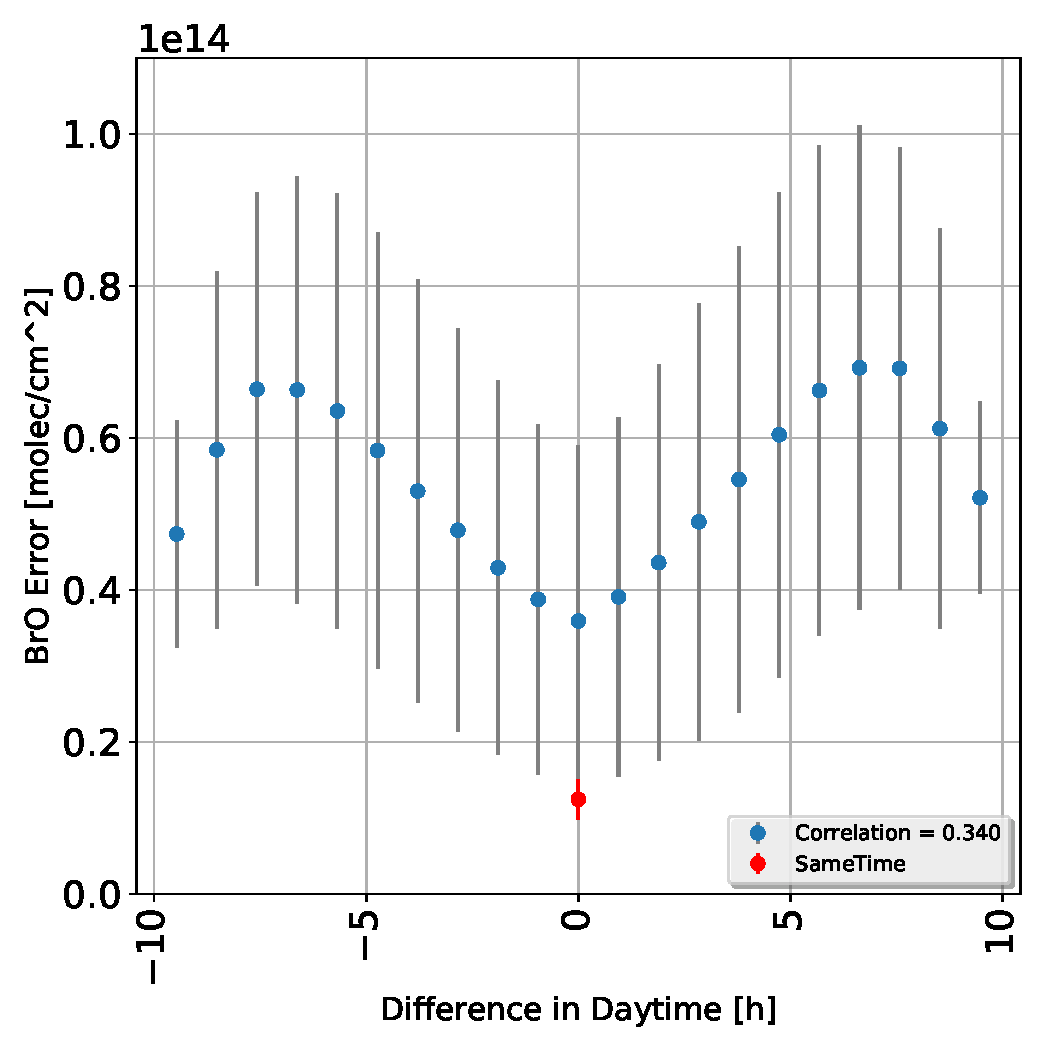
\includegraphics[width=0.3\linewidth]{Bilder/DEpendencoOfBrOErrorOnVariables_absolutedep/D2J2140_0BrOERR_DiffDaytime_Tungu}}
		\subfigure[]{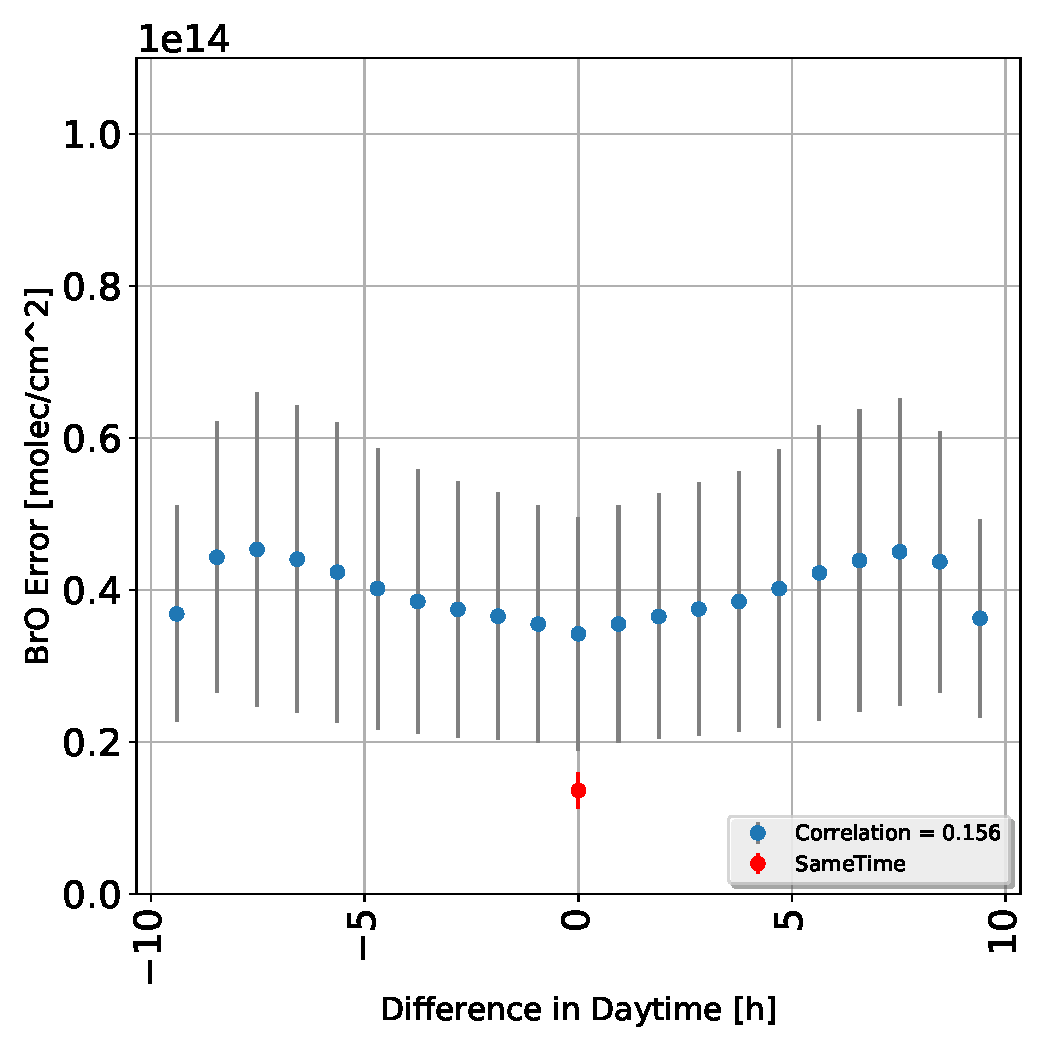
\includegraphics[width=0.3\linewidth]{Bilder/DEpendencoOfBrOErrorOnVariables_absolutedep/I2J8546_0BrOERR_DiffDaytime_Tungu}}
		\subfigure[]{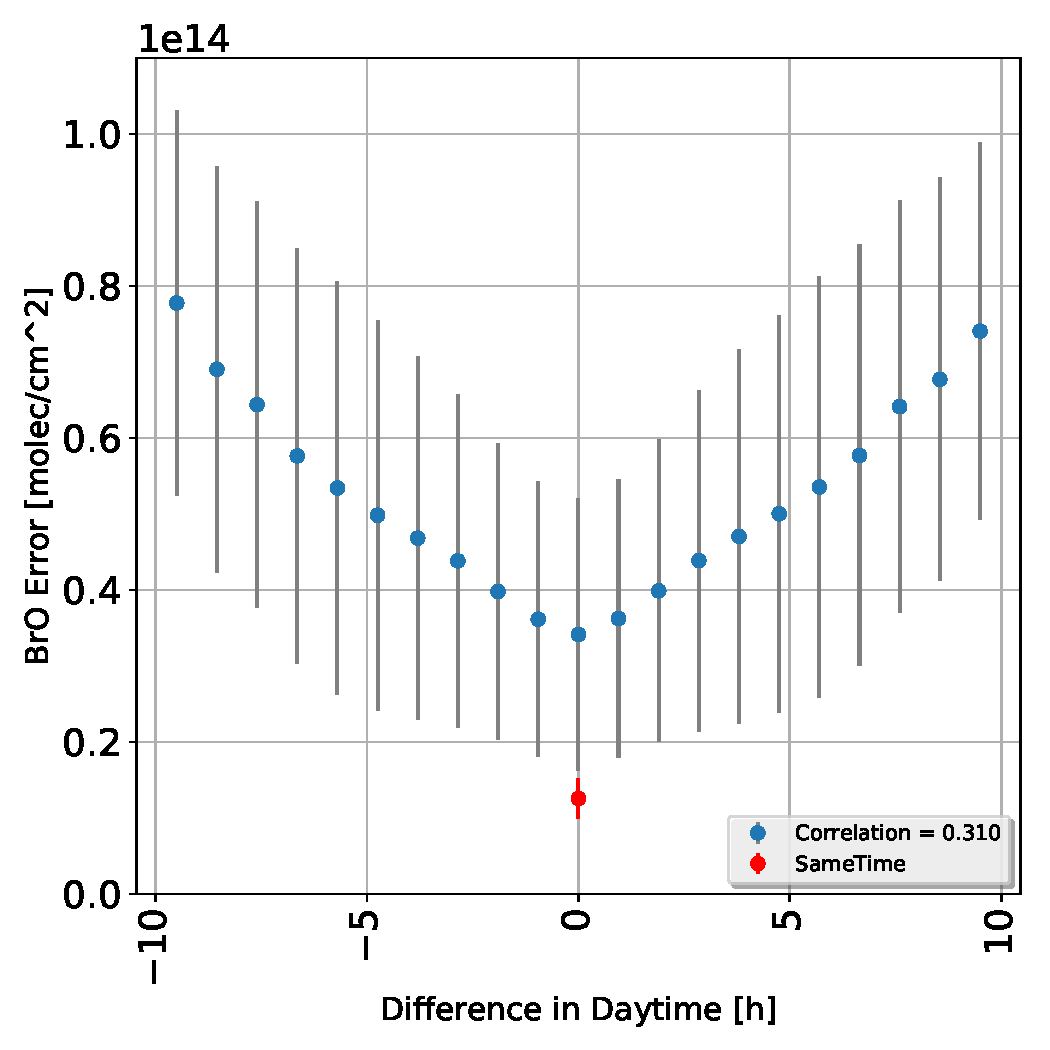
\includegraphics[width=0.3\linewidth]{Bilder/DEpendencoOfBrOErrorOnVariables_absolutedep/I2J8548_0BrOERR_DiffDaytime_Tungu}}
		\centering
		\subfigure[]{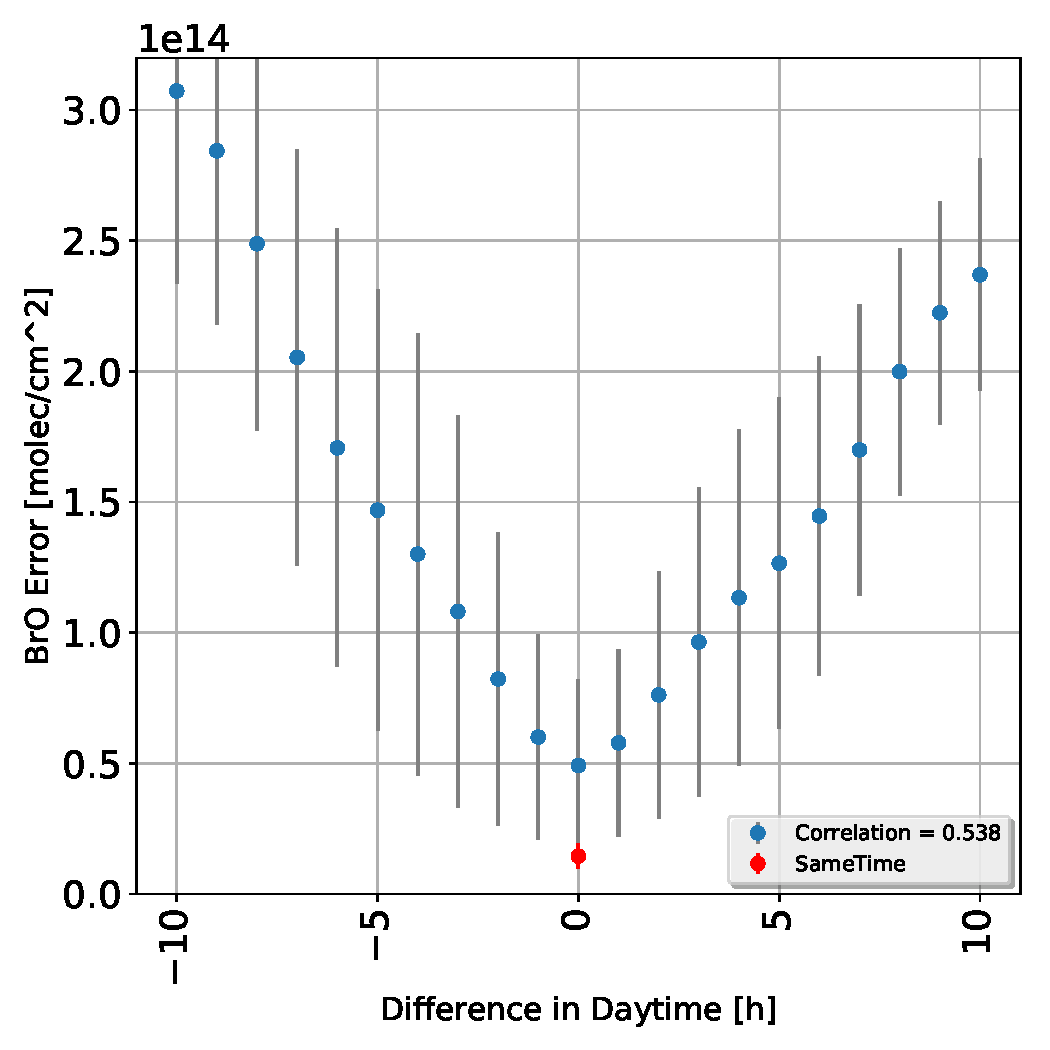
\includegraphics[width=0.3\linewidth]{Bilder/DEpendencoOfBrOErrorOnVariables_absolutedep/D2J2200_0BrOERR_DiffDaytime_Nevad}}
		\subfigure[]{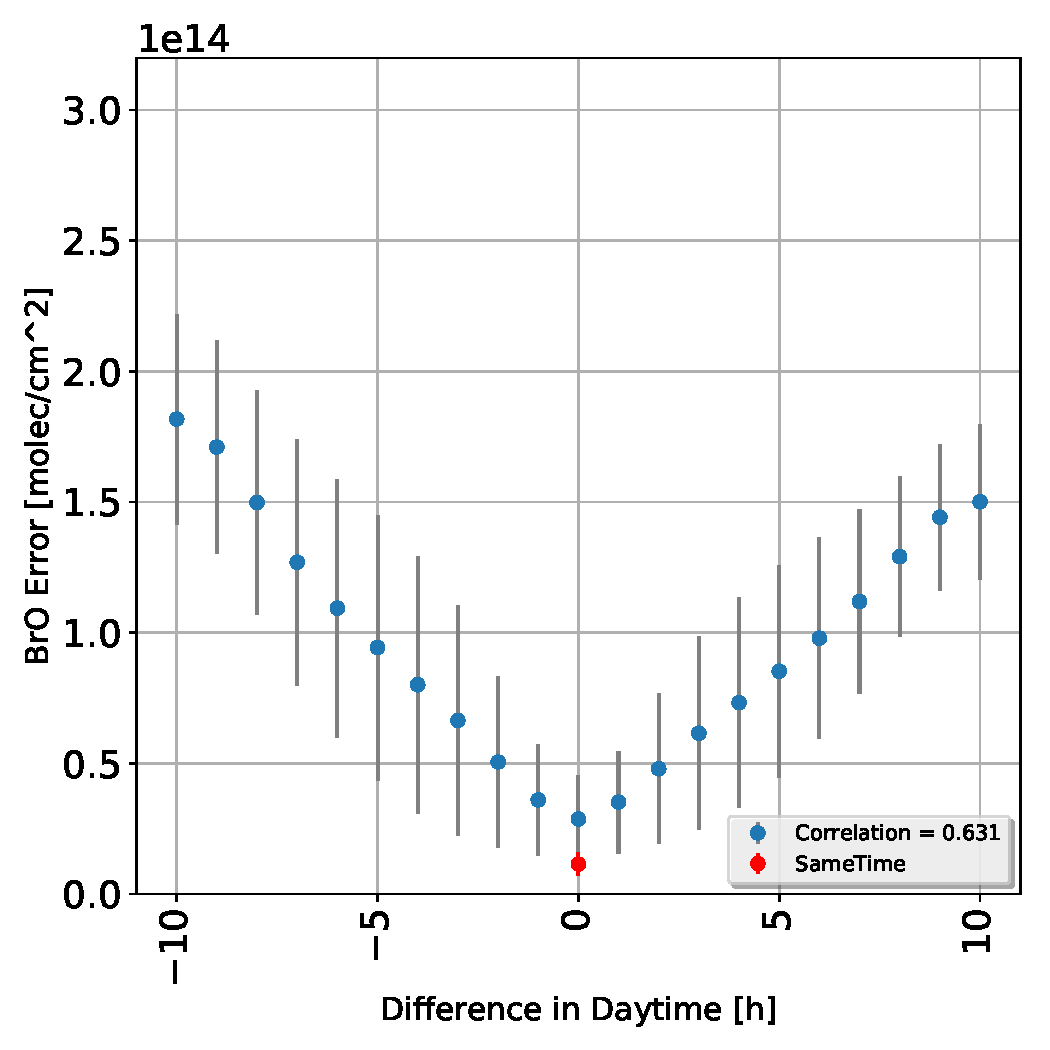
\includegraphics[width=0.3\linewidth]{Bilder/DEpendencoOfBrOErrorOnVariables_absolutedep/D2J2201_0BrOERR_DiffDaytime_Nevad}}
		\caption{The \ce{BrO}  measurement error as a function of the difference of the day time between measuring the reference and the plume are shown. To evaluate the plume spectra all reference spectra with a temporal distance of no longer than two weeks are used. An increase of the \ce{BrO} error with the distance in day time is observable.}
		\label{fig:diffdaytime}
	\end{figure}
	During the day a lot of external parameters like temperature, solar altitude etc. change. In particular the solar altitude could have an impact on the fit quality since the light path of the sun is much longer at the evening than at noon. Therefore the scattering effects and the fraunehofer structures is different for both spectra.\\
	\Cref{fig:diffdaytime} shows the dependency of the \ce{BrO} error on the daytime. The data are calculated as described for the temperature. 
	

	\begin{table}[h]
		\begin{tabular}{|p{2cm}|p{2cm}|p{2cm}|p{2cm}|p{2cm}|p{2cm}|}
			%	\toprule
			Instrument	&D2J2140\_0&I2J8546\_0& I2J8548\_0&D2J2200\_0&D2J2201\_0\\
			\toprule
			Slope&5.07e+12&1.40e+12 &3.77e+12 &2.04e+13& 1.38e+13\\
			\midrule
			Correlation&
			0.340&
			0.156&
			0.310&
			0.538&
			0.631\\
			\midrule
			Zero point& 3.43e+13&3.39e+13&3.28e+13&  4.01e+13&  2.24e+13\\
			\midrule
			$\Delta DT_{2}$&6.8&24.2&8.7&1.9&1.62\\
			\bottomrule
		\end{tabular}
		\label{tab:dtcalc}
		\caption{Results of fitting the dependence of the BrO error on the absolute difference in daytime with in one dimensional polynomial. $\Delta DT_{2}$ is the daytime difference for which the error doubles compared to a same-time-reference. The results differ for every considered instrument.}
	\end{table}

	\begin{table}
	\begin{tabular}{|p{2cm}|p{2cm}|p{2cm}|p{2cm}|p{2cm}|p{2cm}|}
		%	\toprule
		Instrument	&D2J2140\_0&I2J8546\_0& I2J8548\_0&D2J2200\_0&D2J2201\_0\\
		\toprule
		Mean&
		71.97$\equiv$85,1\% &		147.35$\equiv$90,0\%&
		198.4$\equiv$91,4\%&		274.96$\equiv$96,8\%&
		205.8$\equiv$91,2\%\\
		\midrule
		Std&		31.87$\equiv$	89,0\%&31.98 $\equiv$	107,0\%&
		70.96 $\equiv$	109,5\%&		70.78 $\equiv$	101,8\%&
		50.08 $\equiv$	121,6\% \\
		\midrule
		Min&
		6 $\equiv$	75,0\%&		58 $\equiv$	51,3\%
		&91 $\equiv$	93,8\%		&54  $\equiv$	84,4\%
		&45$\equiv$	71,4\%\\
		\midrule
		Max&
		160$\equiv$	94,7\% &
		214 $\equiv$	100,0\% &
		399 $\equiv$	100,0\% &
		433  $\equiv$	100,0\% &
		297 $\equiv$	100,0\% \\
		\bottomrule
	\end{tabular}
	\caption{Remaining amount of References if the maximal accepted daytime difference is 4.75h. The percentages values refer to the decrease of the data relative to \Cref{Tab:refstime}. 4.75h is the mean of the 	$\Delta DT_{2}$s in \cref{tab:dtcalc} without I2J8546\_0 due to the large uncertainty at I2J8546\_0}
	\label{tab:daytimerest}
\end{table}	
%	\begin{table}
%	\begin{tabular}{|p{2cm}|p{2cm}|p{2cm}|p{2cm}|p{2cm}|p{2cm}|}
%		%	\toprule
%		Instrument	&D2J2140\_0&I2J8546\_0& I2J8548\_0&D2J2200\_0&D2J2201\_0\\
%		\toprule
%		Mean&38.98&113.8&153.4&232.38&149.48\\
%		\midrule
%		Std&
%		24.47&
%		50.6&
%		76.87&
%		84.17&
%		72.46\\
%		\midrule
%		Min&1&8&12&3 &6\\
%		\midrule
%		Max&130&213&386&414 &296\\
%		\bottomrule
%	\end{tabular}
%	\caption{maximal Time difference is 3.358$^{\circ}C$,maximal daytime diff is 4.75h without}
%\end{table}	

\Cref{tab:dtcalc} shows equivalent calculations as \cref{tab:tempe}. Since the BrO error plotted against the difference in daytime is symmetric around zero only the absolute differences in daytime are used. These data are fitted with a first order polynomial. The results can be seen in \cref{tab:dtcalc}. Furthermore, the correlations for each instruments and the the differences in daytime where the mean BrO error increases to twice of the zero point ($\Delta DT_{2}$) are shown. To gain more control about the algorithm a maximal daytime difference is defined where the corresponding references are still acceptable. The maximum daytime difference is defined as the mean $\Delta DT_{2}$ of every instrument. Since the data from instrument I2J8546\_0 does not significantly depend on the daytime, this instrument was excluded for the calculation of the mean. Mean($\Delta DT_{2}$) = 4.75. If restricting the data to only references with corresponding daytime of below Mean($\Delta DT_{2}$) we get an averaged decrease of possible references of 9\%. All decreases compared to \cref{Tab:refstime} are listed on \cref{tab:daytimerest}.

	\subsection{Colorindex}
	\begin{figure}
		\subfigure[]{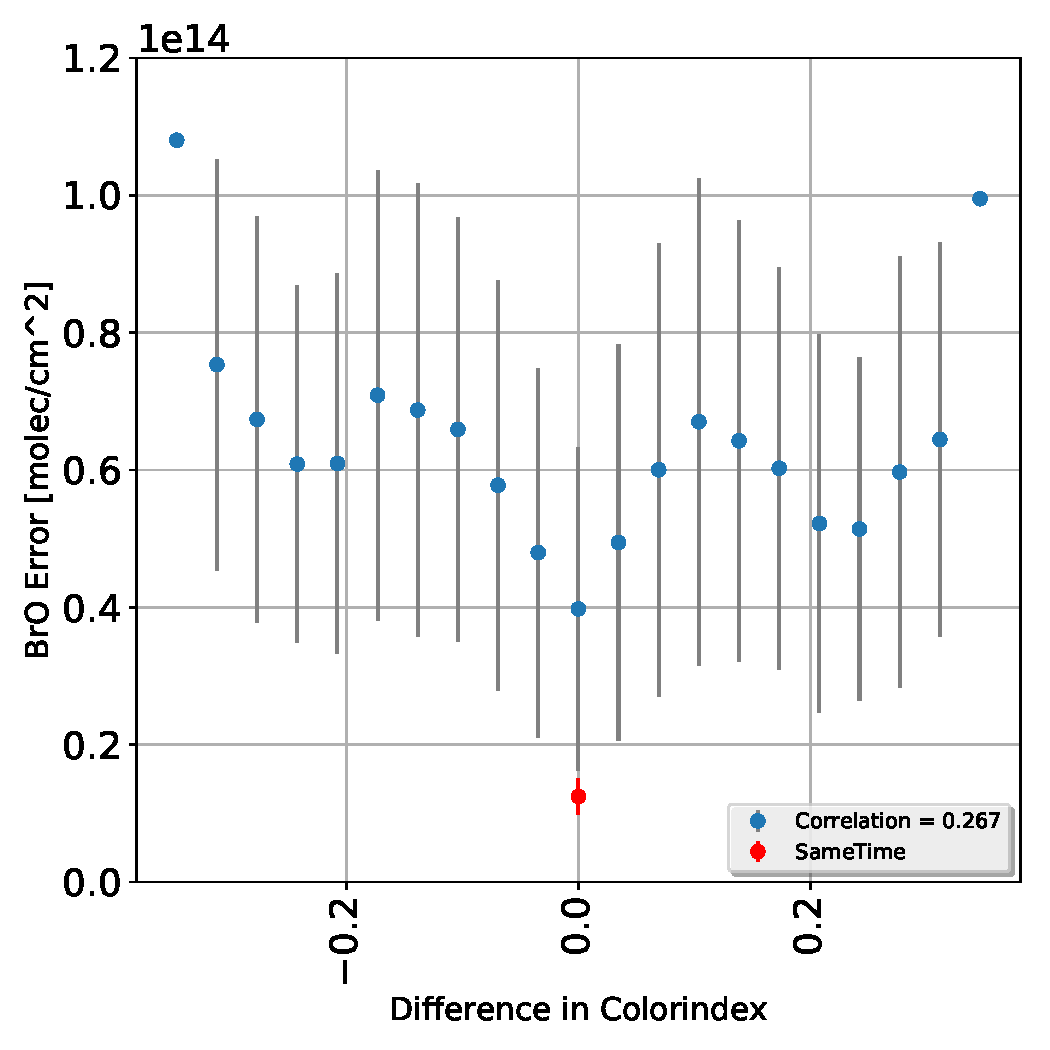
\includegraphics[width=0.3\linewidth]{Bilder/DEpendencoOfBrOErrorOnVariables_absolutedep/D2J2140_0BrOERR_DiffColidx_Tungu}}
		\subfigure[]{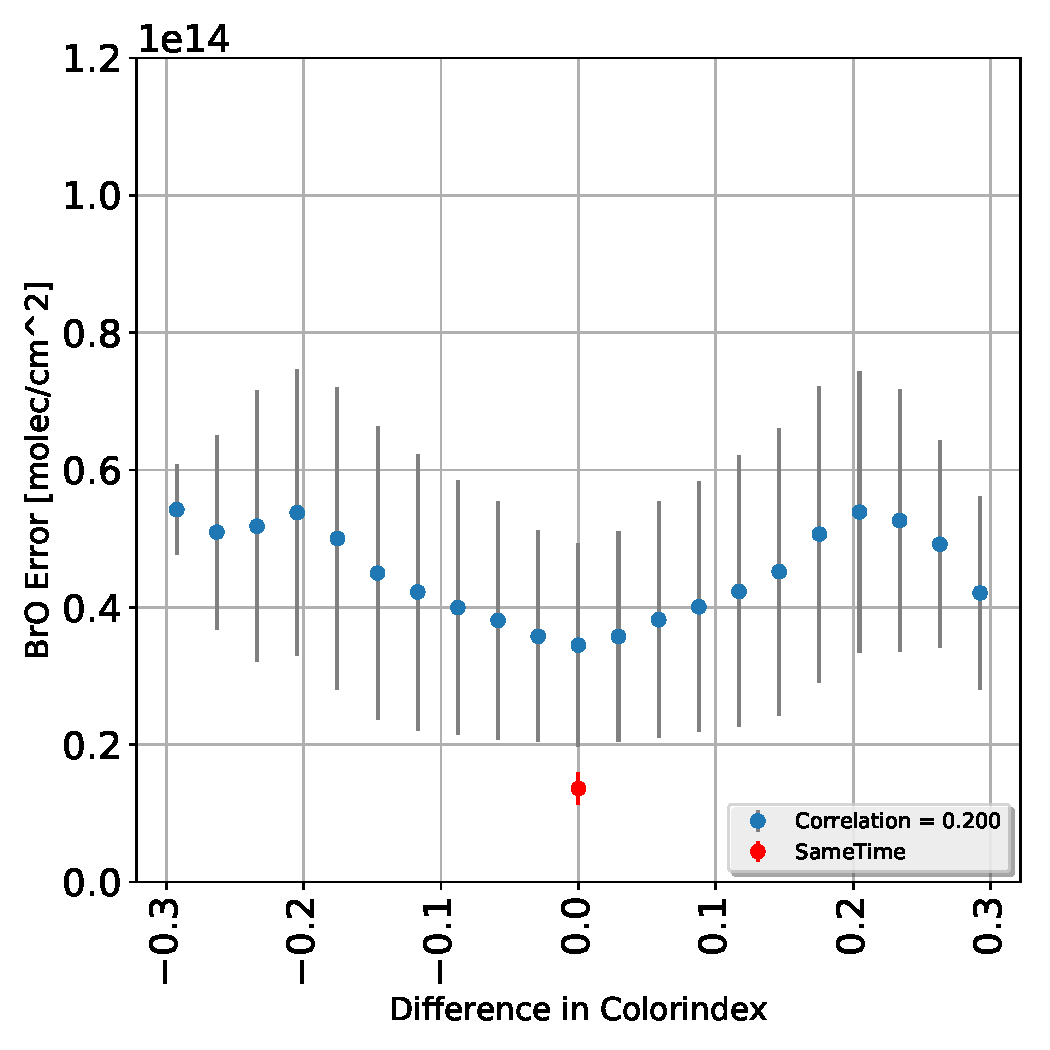
\includegraphics[width=0.3\linewidth]{Bilder/DEpendencoOfBrOErrorOnVariables_absolutedep/I2J8546_0BrOERR_DiffColidx_Tungu}}
		\subfigure[]{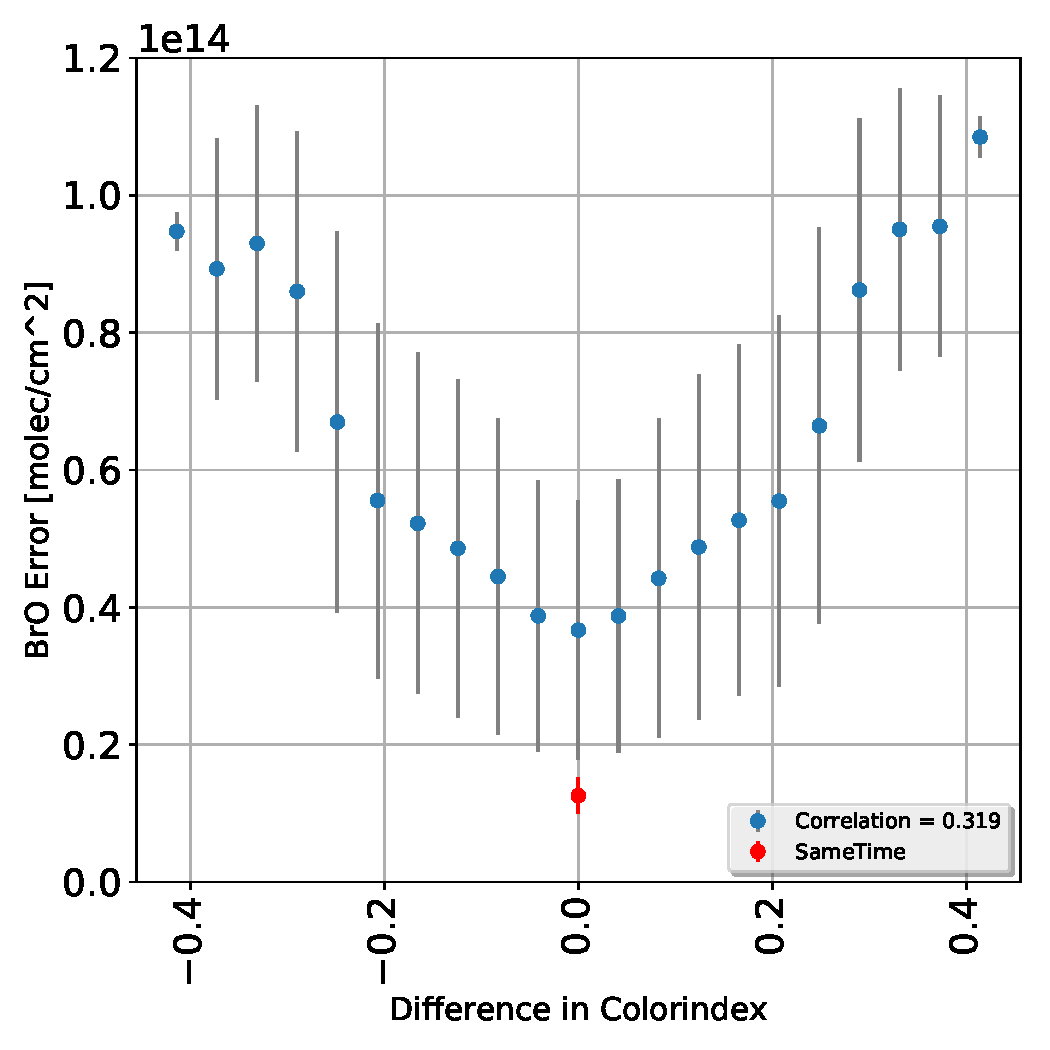
\includegraphics[width=0.3\linewidth]{Bilder/DEpendencoOfBrOErrorOnVariables_absolutedep/I2J8548_0BrOERR_DiffColidx_Tungu}}
		\centering
		\subfigure[]{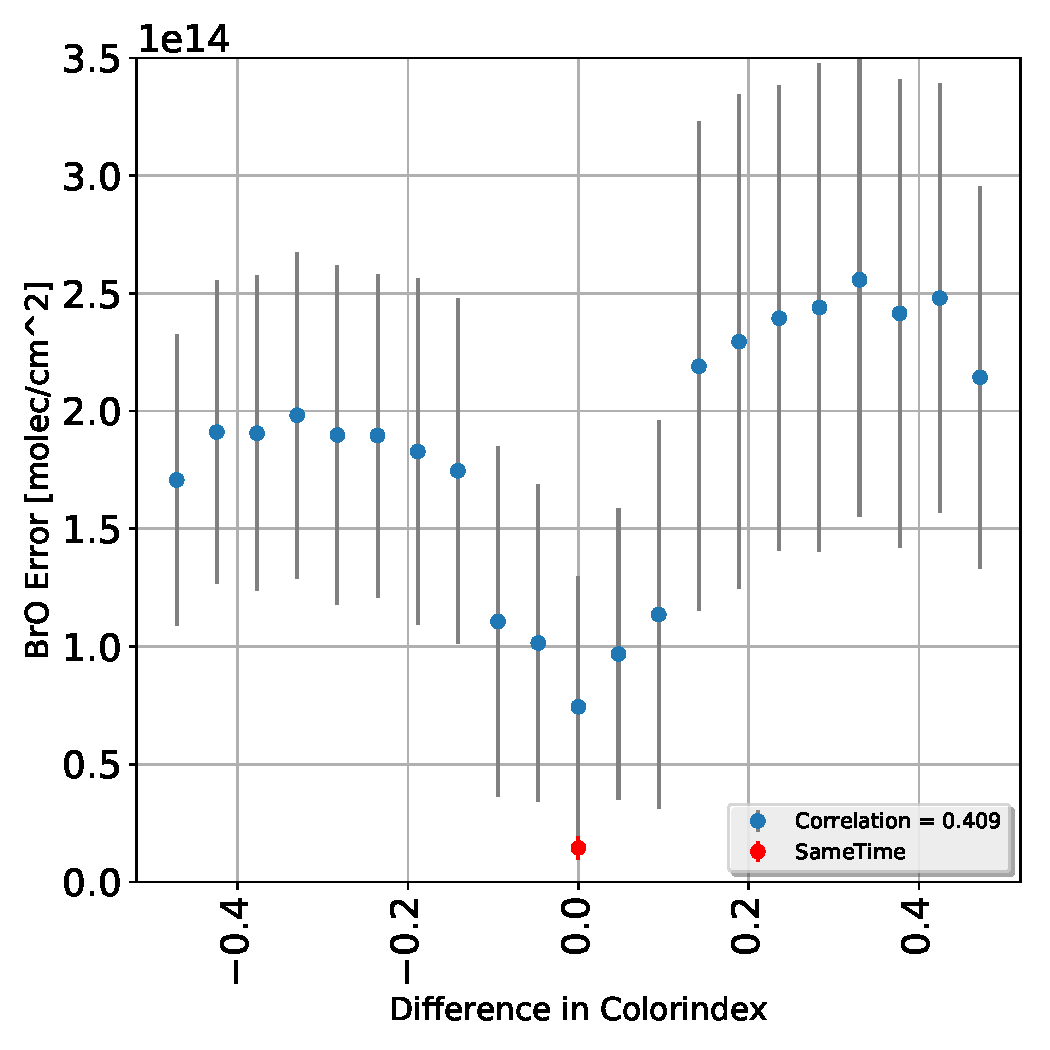
\includegraphics[width=0.3\linewidth]{Bilder/DEpendencoOfBrOErrorOnVariables_absolutedep/D2J2200_0BrOERR_DiffColidx_Nevad}}
		\subfigure[]{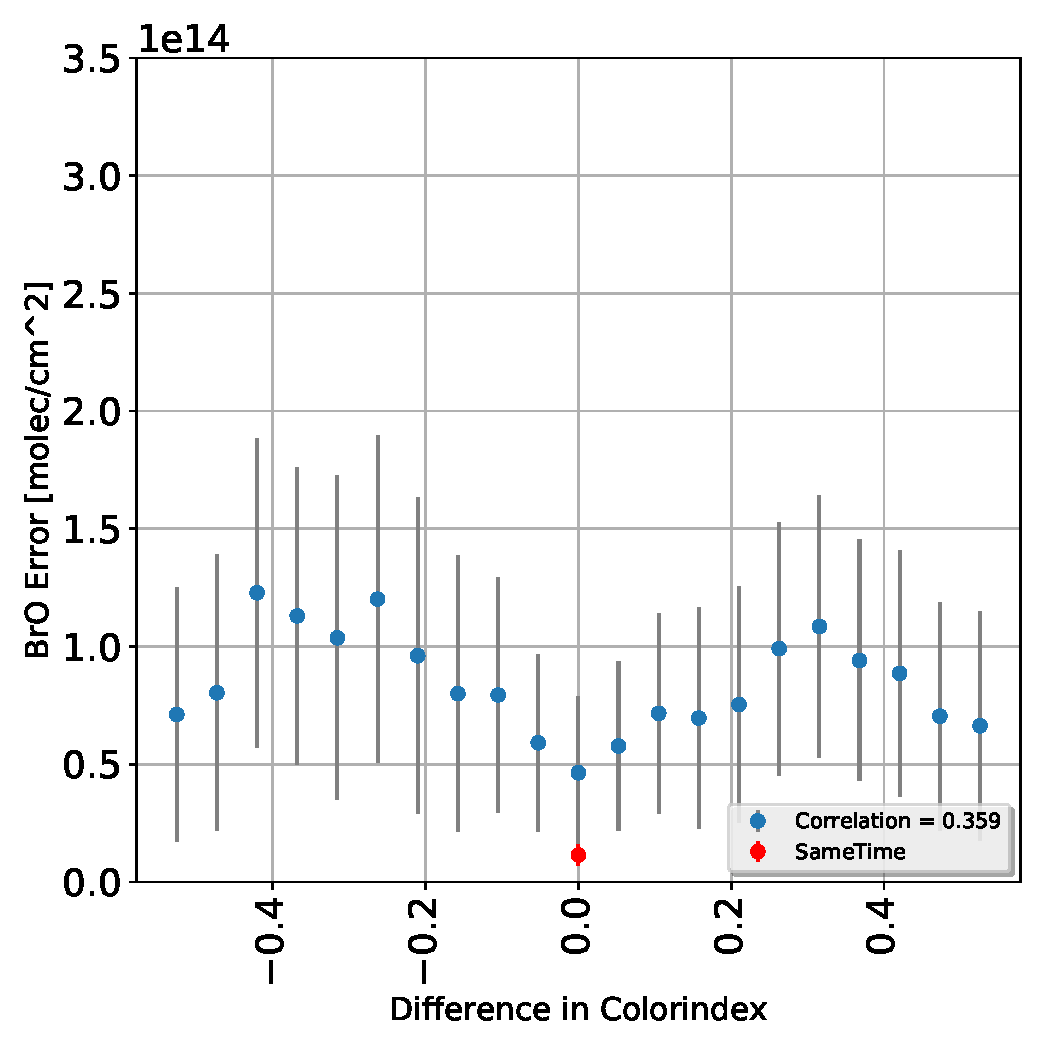
\includegraphics[width=0.3\linewidth]{Bilder/DEpendencoOfBrOErrorOnVariables_absolutedep/D2J2201_0BrOERR_DiffColidx_Nevad}}
		\caption{The \ce{BrO}  measurement error as a function of the difference of colorindex between measuring the reference and the plume are shown. To evaluate the plume spectra all reference spectra with a temporal distance of no longer than two weeks are used. A increase of the \ce{BrO} error with the distance in colorindex is observably.}
		\label{fig:diffcolidx}
	\end{figure}

	Clouds  have  a  strong  influence  on  the  atmospheric  radiative  transfer  and  thus  affect  the  interpretation  and  analysis of DOAS - observations \citep{wagner2014cloud}.
	
	Clouds can be identified by several measurement quantities that they influence.
	As Mie scattering is dominant in clouds the wavelength of the light that is scattered is different than the Rayleigh sky. Thus, clouds can be easily identified by their white color.
	Therefore, the cloudiness of the sky can be quantified in a scalar measure defined by the ratio of the measured intensity at two wavelengths, the so-called colour index.
	\cite{wagner2014cloud} showed that for a zenith-looking instrument the measured radiation intensity is enhanced by clouds. Thus, clouds can cause large errors for the retrieved gas column density and the corresponding uncertainties. 
	Cloud effects are especially severe if the cloudiness for the recorded plume and reference spectra strongly defer. Also for broken clouds the described effect can be observed as measurements at some elevation angles might be influenced by clouds while others are not.
	In this work the Colour Index (CI) is the ratio between the intensities at 320nm and 360 nm.
	These two wavelengths are as far apart as the filter used for stray-light prevention in the spectrometers allows.
	%% I don’t understand 	
	On the other hand, the lower wavelength avoids the deep UV range where \ce{SO2} and  \ce{O3} absorption plays a dominant role.
	%% I don’t understand 	
	The Mie scattering in the clouds is responsible for the higher amount of radiation from larger wavelengths. This results in a decrease of the CI \citep{lubcke2014optical}.
	\\
	We evaluated the CI at the zenith, to increase the stability of the fit we added in each cases 10 intensitys. Using always the zenith to evaluate the colour index makes the colour index more comparable, but if broken clouds occur, the CI of the reference and the plume could differ from the calculated CI of the zenith. This could be a reason for the large deviations of the mean \ce{BrO} error as function of the colour index (see \Cref{fig:diffcolidx})
	\begin{itemize}
		\item The \ce{BrO}  error as a function of the difference in colour index is also symmetric around zero for all observed instruments, thus the absolute difference in colour index is sufficient for the evaluating.
		\item The \ce{BrO}  error decreases for extreme differences in colour index for almost all instruments, the only exception is the  I2J8548\_0 at Tungurahua. Especially at D2J2140\_0 the curve is not monotonically increasing with increasing difference in colorindex. Even though  D2J2140\_0 is symmetric around zero.
	\end{itemize}
	\begin{itemize}
		\item 	The \ce{BrO} error increases with the Colorindex differences as \\
		\begin{align*}
		\rightarrow&  BrO_{Error} = f(ext. P)+ 1.01\cdot10^{13}\cdot\frac{\Delta Cidx}{0.1} + \mathcal{O}\left(\right) & Tungurahua\\
		\rightarrow&  BrO_{Error} = f(ext. P)+  4\cdot10^{13}\cdot\frac{\Delta Cidx}{0.1} + \mathcal{O}\left(\right) & Nevado Del Ruiz\\
		\end{align*}
	\end{itemize}
	\begin{table}[h]
	\begin{tabular}{|p{2cm}|p{2cm}|p{2cm}|p{2cm}|p{2cm}|p{2cm}|}
			%	\toprule
			Instrument	&D2J2140\_0&I2J8546\_0& I2J8548\_0&D2J2200\_0&D2J2201\_0\\
			\toprule
			Slope&2.30e+14 &7.92e+13 &1.17e+14 &5.42e+14&1.91e+14\\
			\midrule
			Correlation&
			0.267&
			0.200&
			0.319&
			0.409&
			0.359\\
			\midrule
			Zero point&4.01e+13&3.36e+13&3.47e+13& 7.21e+13& 4.74e+13\\
						\midrule
			$\Delta CI_{2}$&0.174&0.424&0.297&0.133&0.248\\
			\bottomrule
		\end{tabular}
		\label{tab:colidxcalc}
	\end{table}


	\begin{table}[h]
	\begin{tabular}{|p{2cm}|p{2cm}|p{2cm}|p{2cm}|p{2cm}|p{2cm}|}
		% 	\toprule
		Instrument	&D2J2140\_0&I2J8546\_0& I2J8548\_0&D2J2200\_0&D2J2201\_0\\
		\toprule
		Mean&
		84.6$\equiv$ 100,0\% &	163.7$\equiv$ 100,0\%&	215.6$\equiv$99,3\%&
		275.4$\equiv$97,0\% &219.4$\equiv$97,3\% \\
		\midrule
		Std&
		35.8$\equiv$100,0\% &	29.9$\equiv$	100,0\% &
		65.4$\equiv$	100,9\%&
		67.8$\equiv$	97,6\% &
		49.86$\equiv$	121,0\% \\
		\midrule
		Min&
		8$\equiv$	100,0\% &
		113$\equiv$	100,0\% 
		&97$\equiv$	100,0\% 
		&61 $\equiv$	95,3\% 
		&28	$\equiv$44,4\% \\
		\midrule
		Max
		&169$\equiv$	100,0\% 
		&214$\equiv$	100,0\% 
		&399$\equiv$	100,0\% 
		&421 $\equiv$	97,2\% 
		&297 $\equiv$	100,0\%  \\
		\bottomrule
	\end{tabular}
	\caption{Amount of Possible references while restricting the difference in colorindex  between plume and reference to differences above 0.2553.}
	\label{tab:colidxres}
\end{table}	


	\begin{table}
	\begin{tabular}{|p{2cm}|p{2cm}|p{2cm}|p{2cm}|p{2cm}|p{2cm}|}
		%	\toprule
		Instrument	&D2J2140\_0&I2J8546\_0& I2J8548\_0&D2J2200\_0&D2J2201\_0\\
		\toprule
		Mean&38.98&113.8&153.2&223.8&149.37\\
		\midrule
		Std&
		24.47&
		50.6&
		76.78&
		82.5&
		72.41\\
		\midrule
		Min&1&8&12&3 &6\\
		\midrule
		Max&130&213&386&399 &296\\
		\bottomrule
	\end{tabular}
	\caption{Amount of Possible references while restricting the difference in colorindex  between plume and reference to differences above 0.2553. maximal Time difference is 3.358$^{\circ}C$,maximal daytime diff is 4.75h without}
\end{table}	
As for the temperature and the daytime the BrO error fas fitted on the absolute differences in colorindex with an polynomial of the first grad for each instrument. The absolute difference can be taken due to the symetric around zero as it  can be seen in \cref{fig:diffcolidx}. The results including the slope, zero point, correlation and the colorindex where the BrO error increases to twice of the zero point ($\Delta CI_{2}$) are listed an \cref{tab:colidxcalc}.
The data were restricted to references where the corresponding colorindex difference is below the mean of the $\Delta CI_{2}$ = 0.256. The remaining number of references compared to \cref{Tab:refstime} can be found in \cref{tab:colidxres}


		\subsection{Elevation Angle}
	\begin{figure}
		\subfigure[]{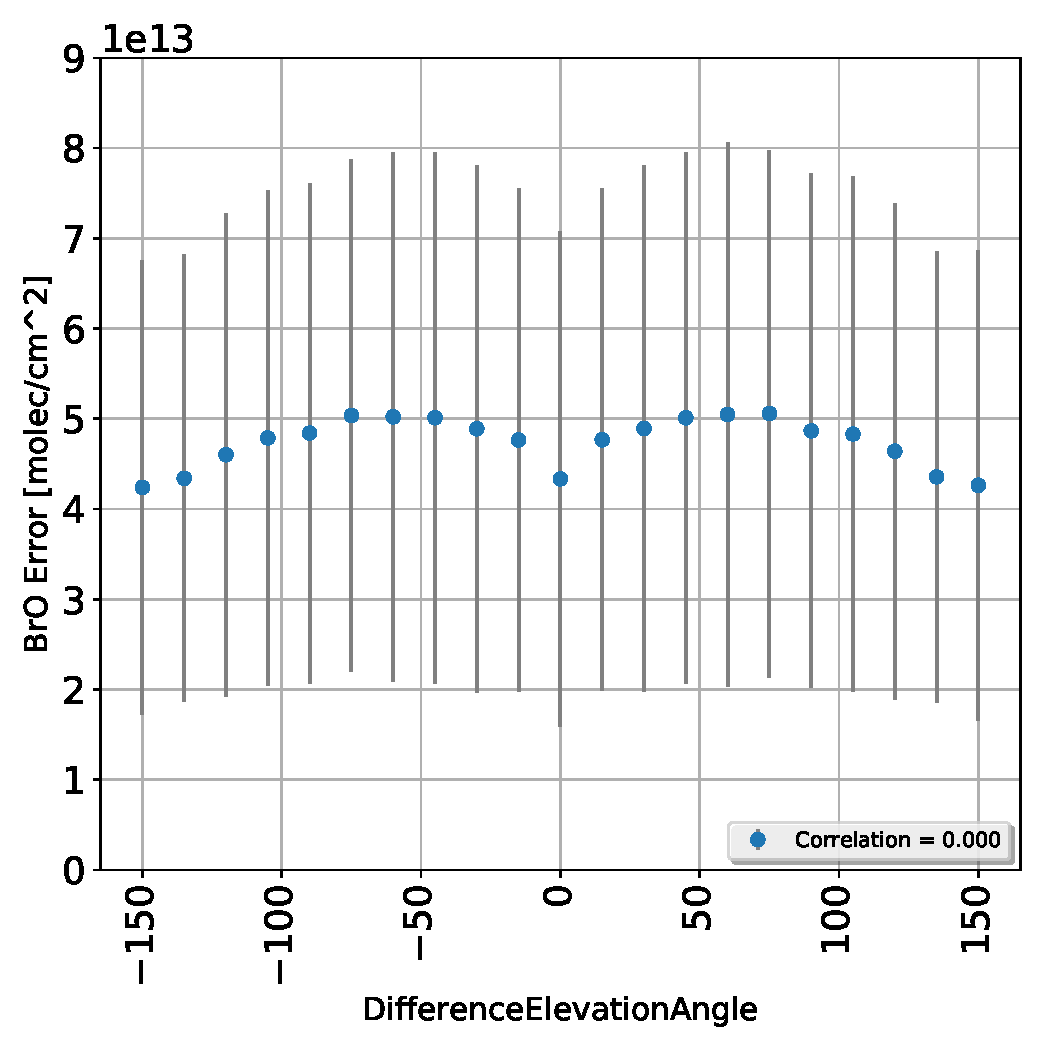
\includegraphics[width=0.3\linewidth]{Bilder/DEpendencoOfBrOErrorOnVariables_absolutedep/D2J2140_0BrOERR_DiffElevAngle_Tungu}}
		\subfigure[]{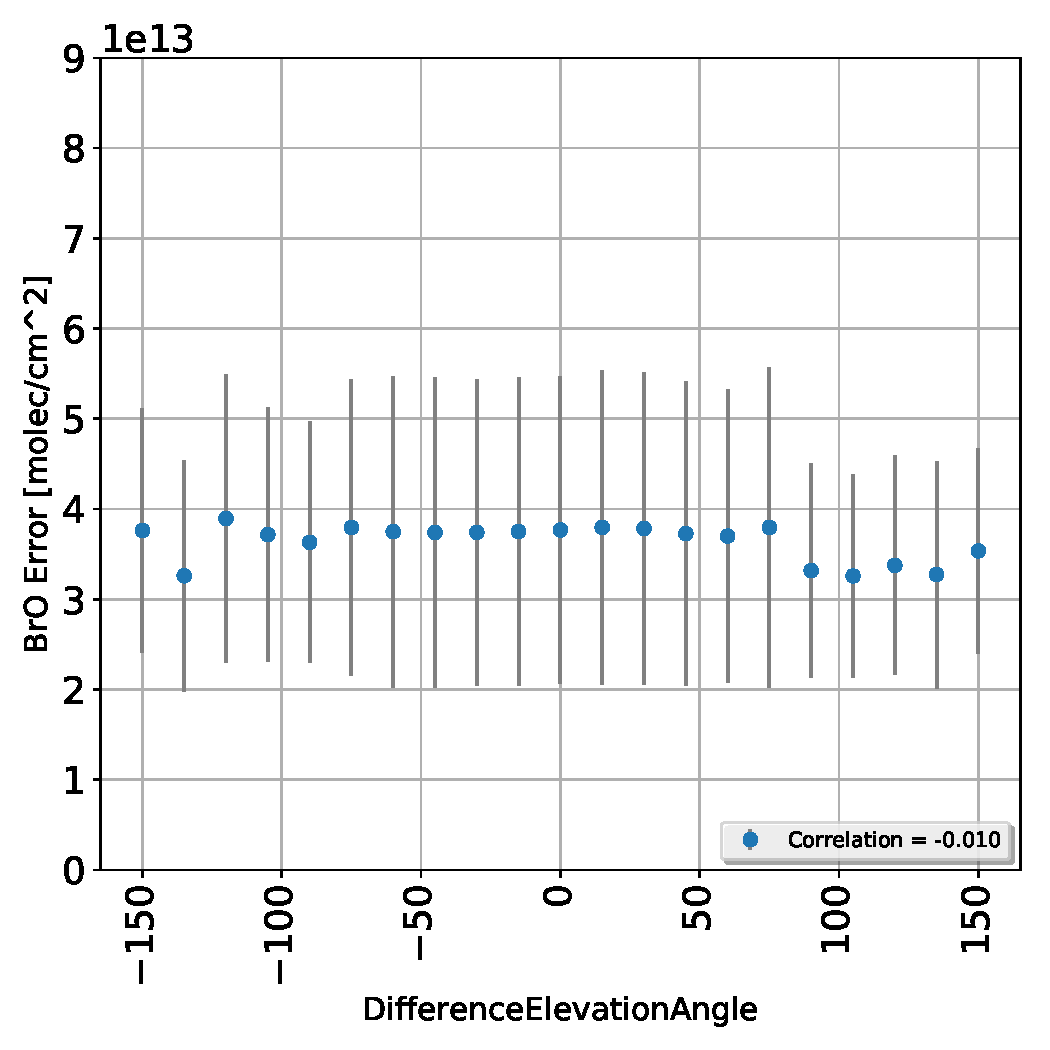
\includegraphics[width=0.3\linewidth]{Bilder/DEpendencoOfBrOErrorOnVariables_absolutedep/I2J8546_0BrOERR_DiffElevAngle_Tungu}}
		\subfigure[]{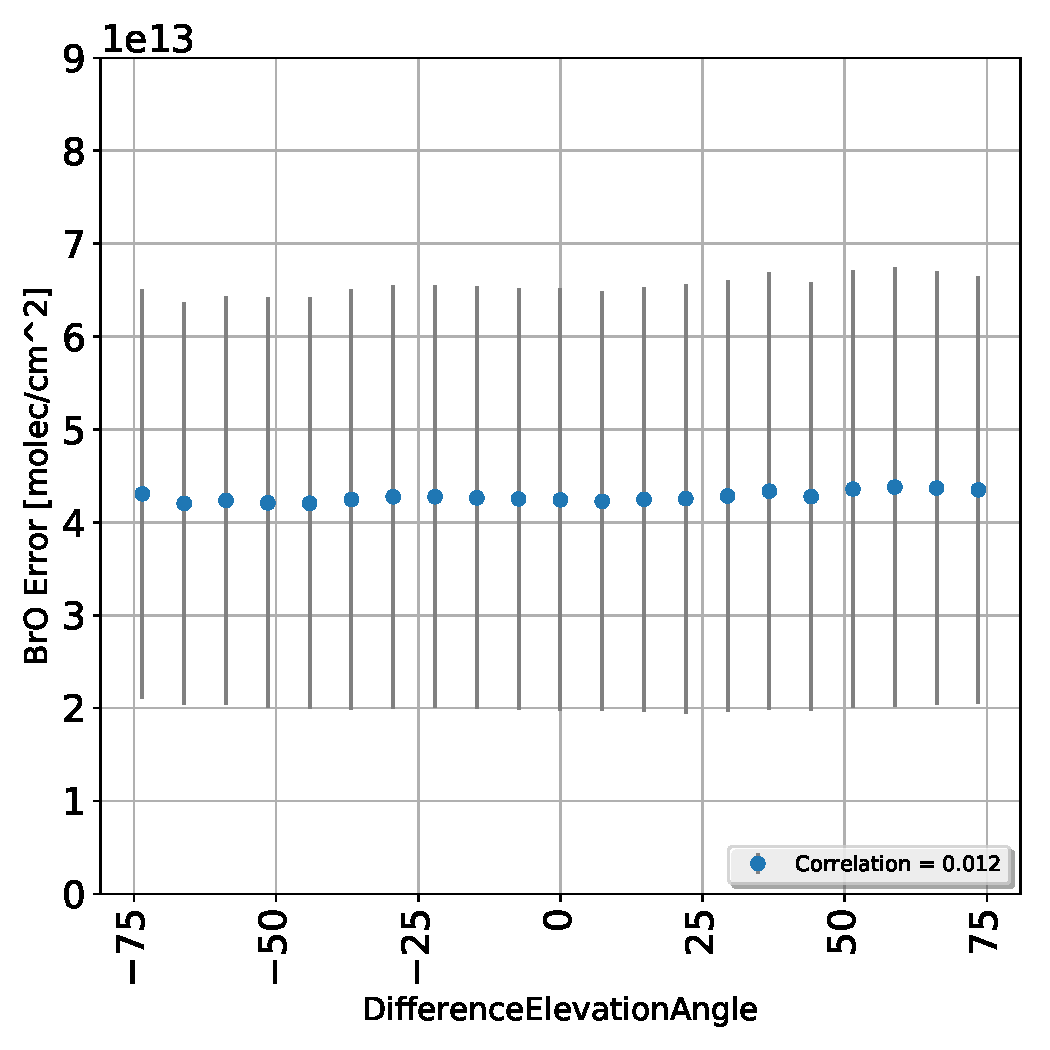
\includegraphics[width=0.3\linewidth]{Bilder/DEpendencoOfBrOErrorOnVariables_absolutedep/I2J8548_0BrOERR_DiffElevAngle_Tungu}}
		\centering
		\subfigure[]{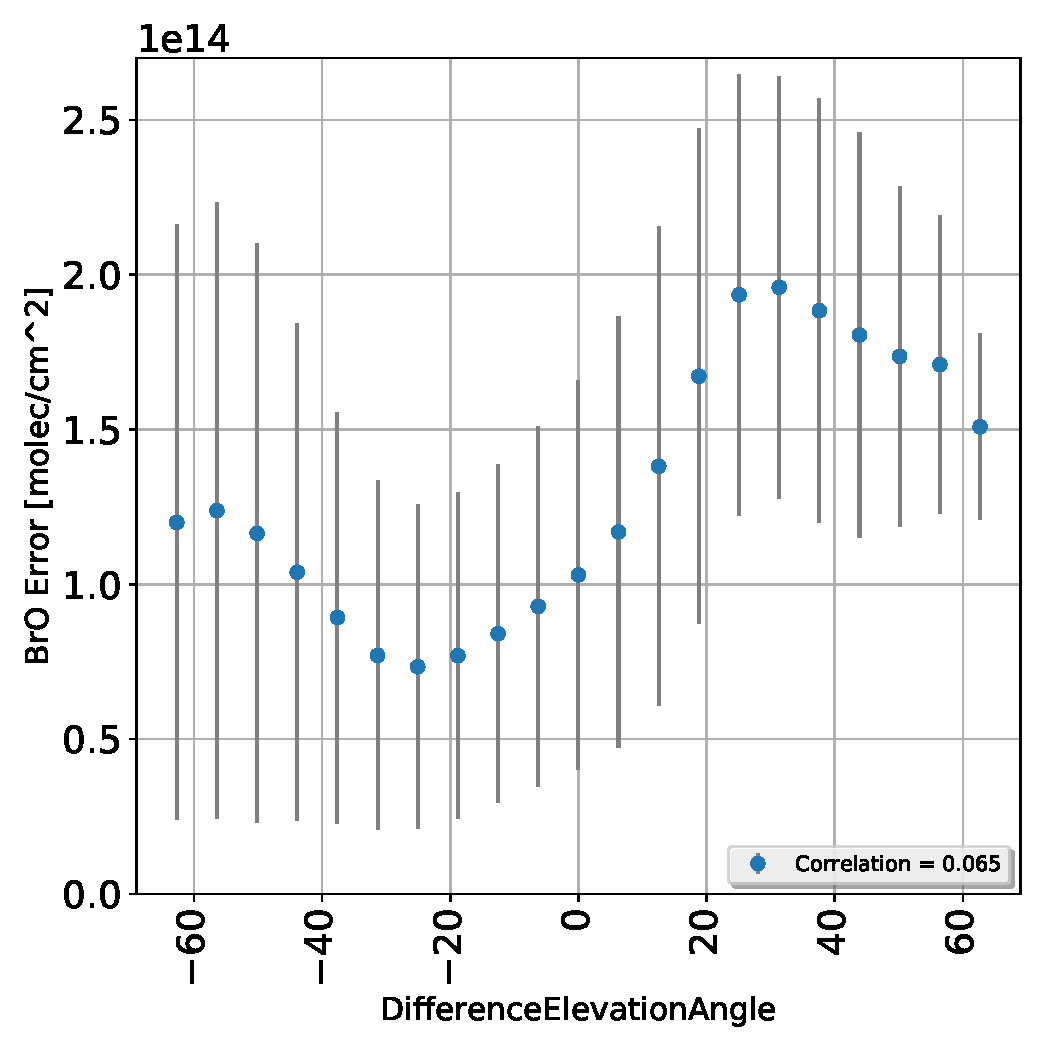
\includegraphics[width=0.3\linewidth]{Bilder/DEpendencoOfBrOErrorOnVariables_absolutedep/D2J2200_0BrOERR_DiffElevAngle_Nevad}}
		\subfigure[]{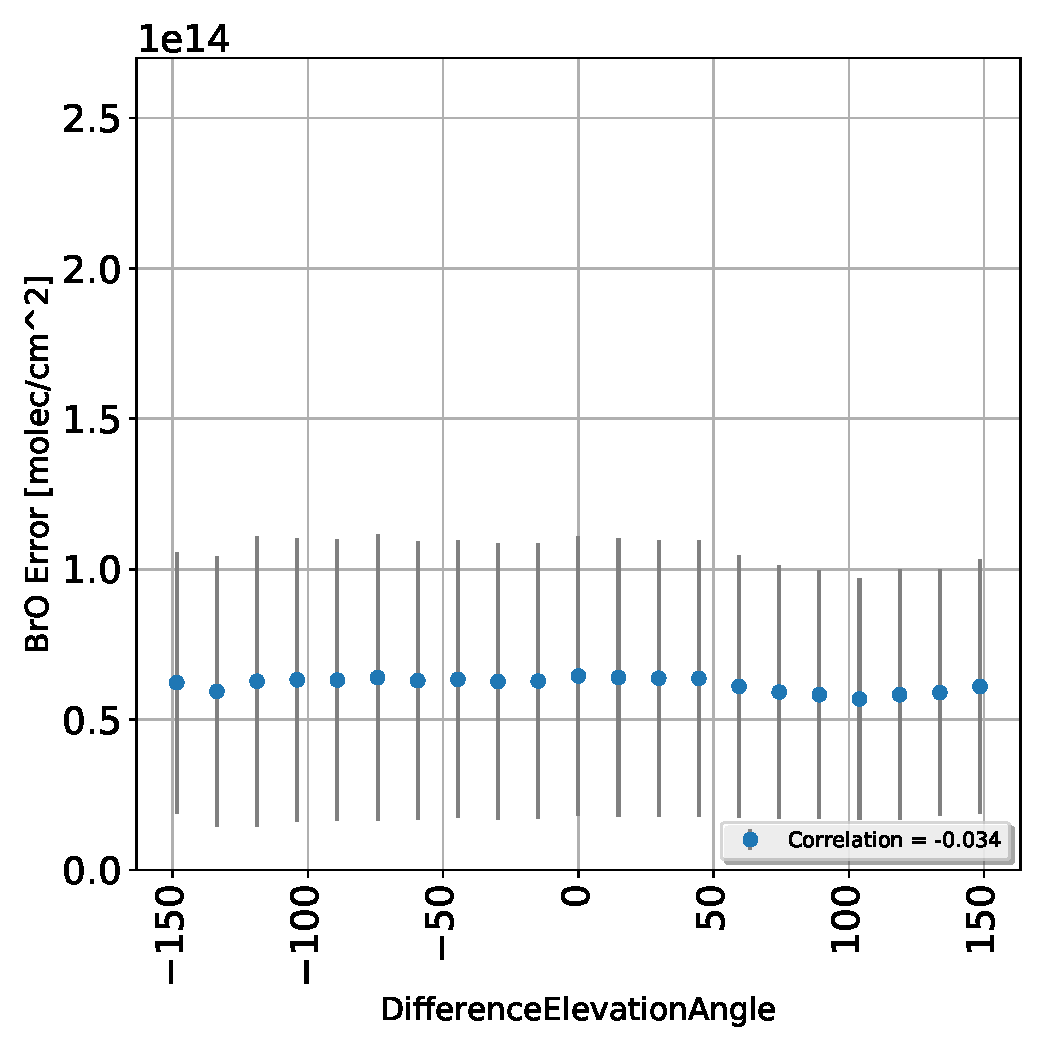
\includegraphics[width=0.3\linewidth]{Bilder/DEpendencoOfBrOErrorOnVariables_absolutedep/D2J2201_0BrOERR_DiffElevAngle_Nevad}}
		\caption{The \ce{BrO}  measurement error as a function of the Elevation Angle. To evaluate the plume spectra all reference spectra with a temporal distance of no longer than two weeks are used. We can't see any significant correlation.}
		\label{fig:diffeleangle}
	\end{figure}
	The elevation angle describes the angle between the horizon and the zenith. When using the plume spectrum and the reference spectrum of the same time, the difference in elevation angle cannot be zero, since the location of the plume does not coincidence with the location of the reference.\\
	As can be seen in \cref{fig:diffeleangle} the \ce{BrO} error does not depend significantly on the difference between the Elevation Angles. This could have several reasons. One problem is, that the Elevation Angle of Plume and Reference spectrum is not the same. This could also be a reason of uncertainty of the evaluations of the plume spectrum.
	Only the data of the D2J2200\_0 instrument vary with the elevation angle. The observable variation of the BrO error with the elevation angle differs from the symmetric dependence of all other external parameter, the minimum BrO error can be found at a difference in elevation angle of -20$^{\circ}$. This curve is a result of the solar altitude over the day which can be seen if we only use data of the same day time. Such a plot can be seen in \cite{fig:d2j22000diffelevangleonetempnevad}.
	\begin{figure}
		\subfigure{
		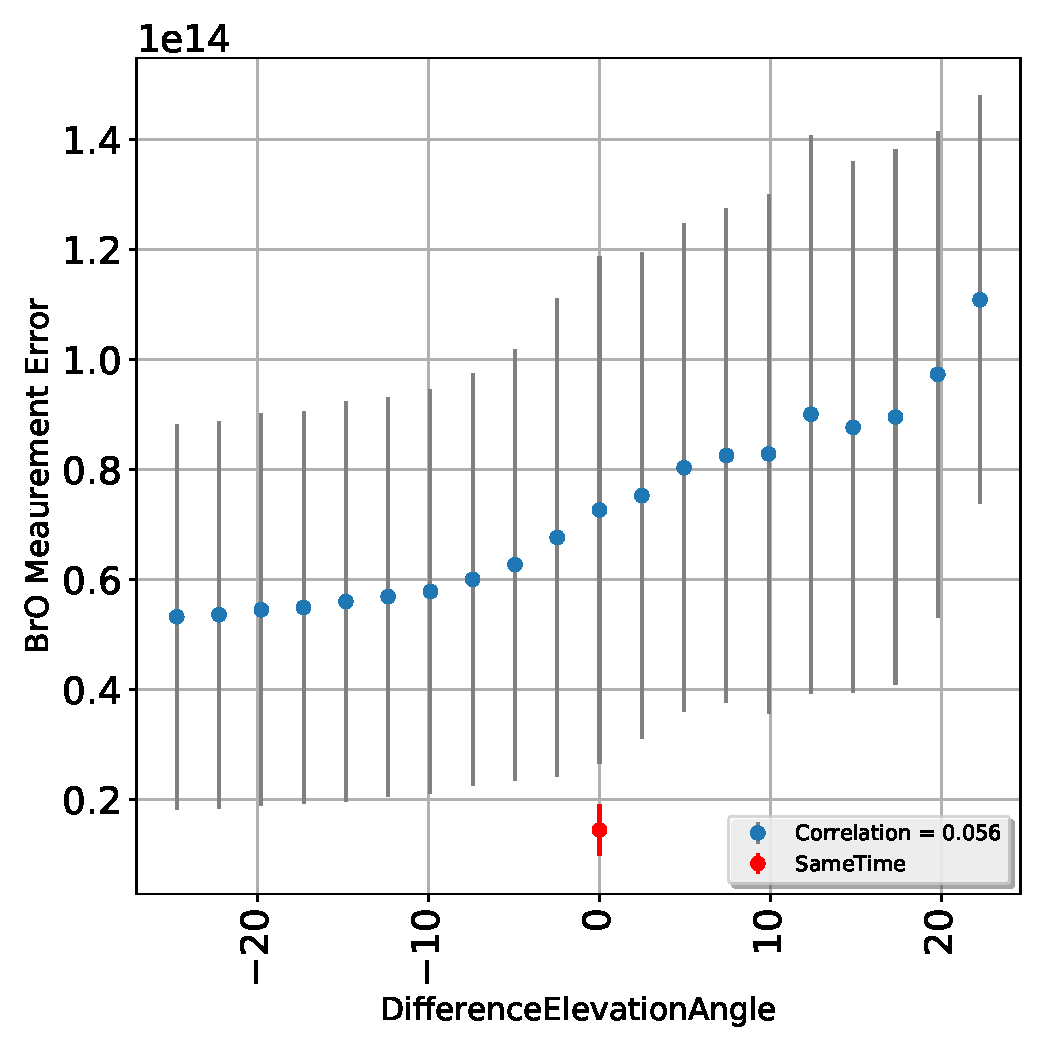
\includegraphics[width=0.49\linewidth]{Bilder/D2J2200_0_DiffElevAngle_onedaytime_Nevad}}
		\subfigure{
		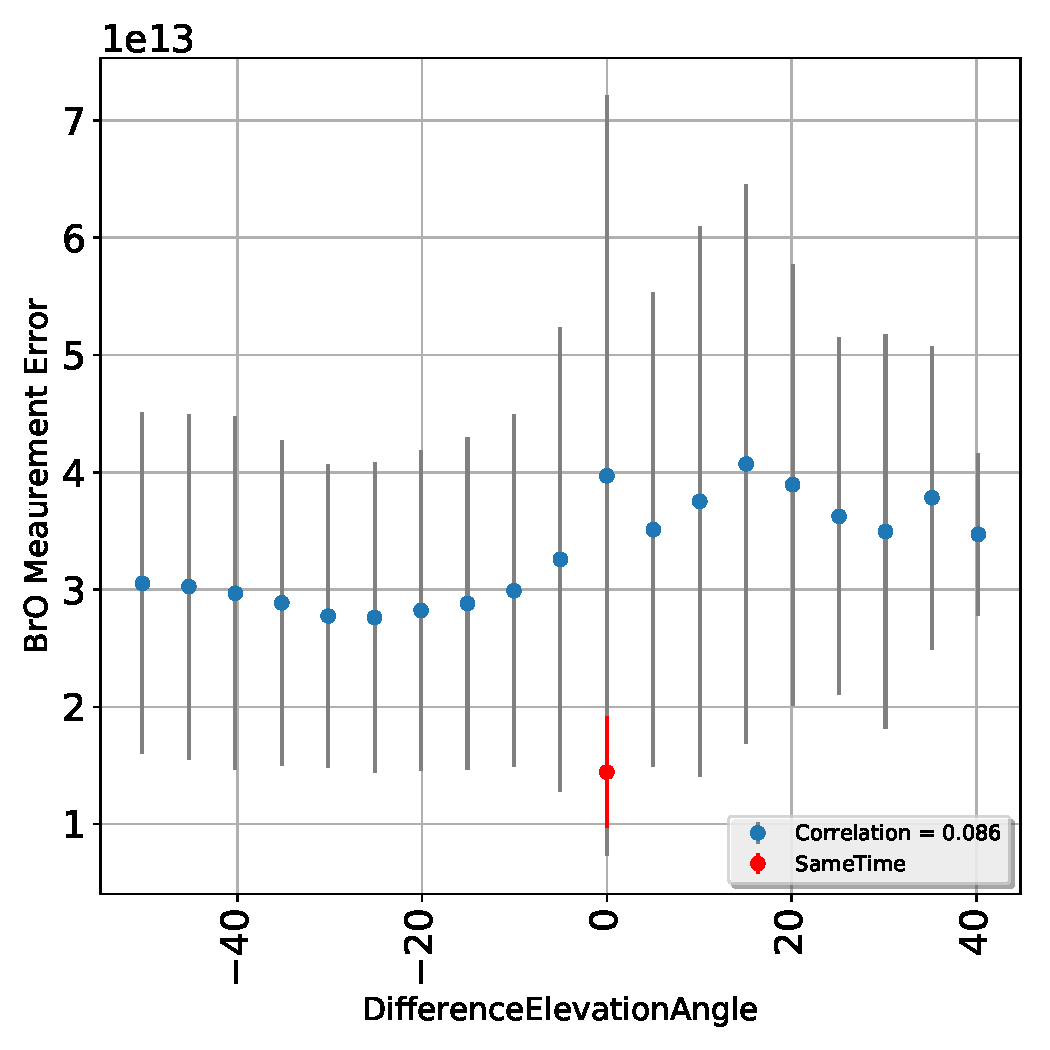
\includegraphics[width=0.49\linewidth]{Bilder/D2J2200_0_DiffElevAngle_onetemp_Nevad}}
		\caption{Left: constant daytime,right: constant temperature}
		\label{fig:d2j22000diffelevangleonetempnevad}
	\end{figure}
	
	\begin{itemize}
		\item The \ce{BrO}  error as a function of the difference in colour index is also symmetric around zero for all instruments, except  D2J2200\_0 at Nevado Del Ruiz. 
		\item Only D2J2140\_0 shows a minimum of the \ce{BrO}  error at a difference in Elevation Angle of 0$^{\circ}$. The \ce{BrO}  error curve from D2J2200\_0 shows a minimum at around -20$^{\circ}$.
		\item Because there is no significant dependence between \ce{BrO}  error and the difference in Elevation Angle it will not be considered in further analysis.
	\end{itemize}
	\begin{table}[h]
		\begin{tabular}{|p{2cm}|p{2cm}|p{2cm}|p{2cm}|p{2cm}|p{2cm}|}
			%	\toprule
			Instrument	&D2J2140\_0&I2J8546\_0& I2J8548\_0&D2J2200\_0&D2J2201\_0\\
			\toprule
			Slope& 1.73e+8& 1.55e+10  &-9.00e+9 &2.92e+11&-3.96e+10\\
			\midrule
			Correlation&
			0.000&
			-0.010&
			0.012&
			0.065&
			-0.034\\
			\midrule
			Zero point&4.77e+13&4.23e+13&3.78e+13&8.37e+13 &6.44e+13 \\
			\bottomrule
		\end{tabular}
	\end{table}
	Since the BrO error does not depend noticeable on the Elevation Angle no restriction on differences of the elevation angle are needed.
	\subsection{Exposure Time}
	\begin{figure}
		\subfigure[]{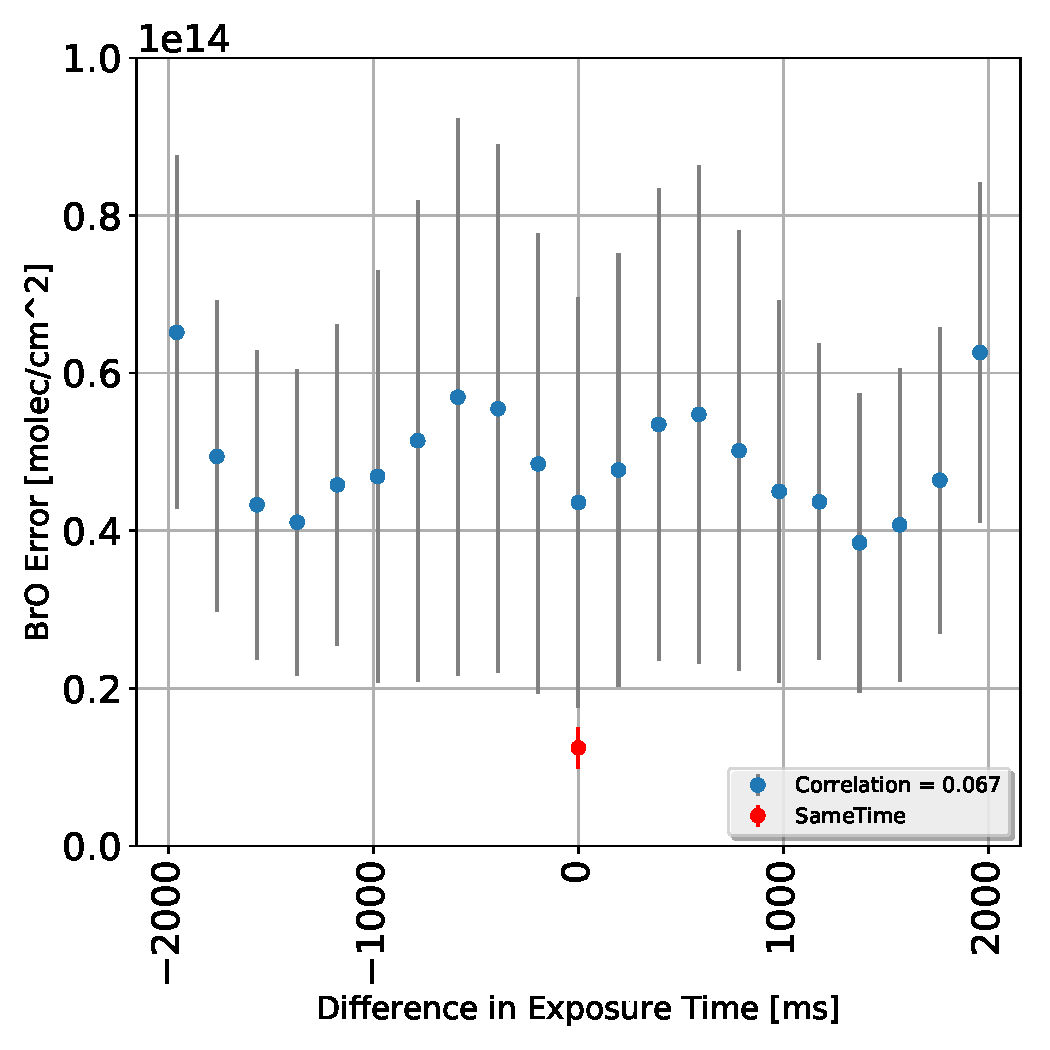
\includegraphics[width=0.3\linewidth]{Bilder/DEpendencoOfBrOErrorOnVariables_absolutedep/D2J2140_0BrOERR_DiffExpTime_Tungu}}
		\subfigure[]{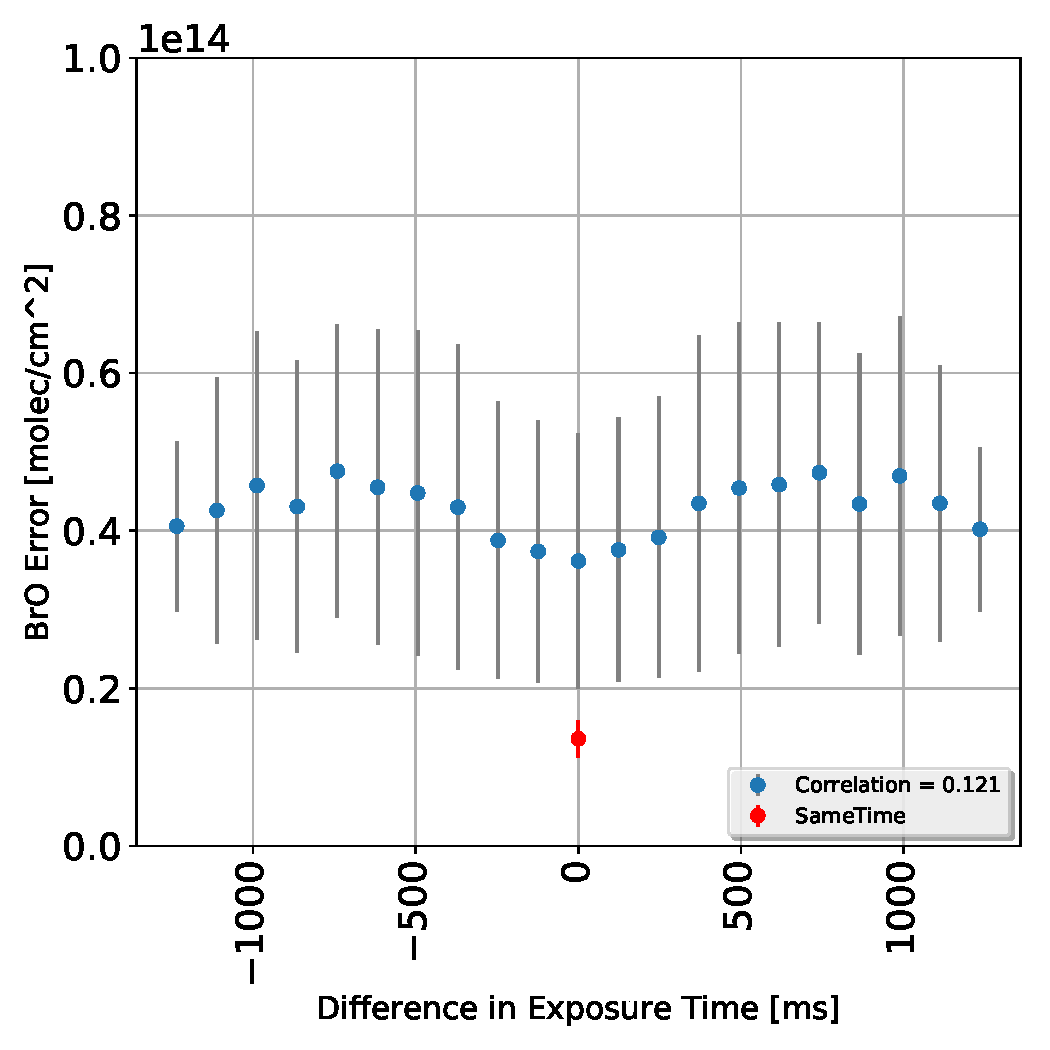
\includegraphics[width=0.3\linewidth]{Bilder/DEpendencoOfBrOErrorOnVariables_absolutedep/I2J8546_0BrOERR_DiffExpTime_Tungu}}
		\subfigure[]{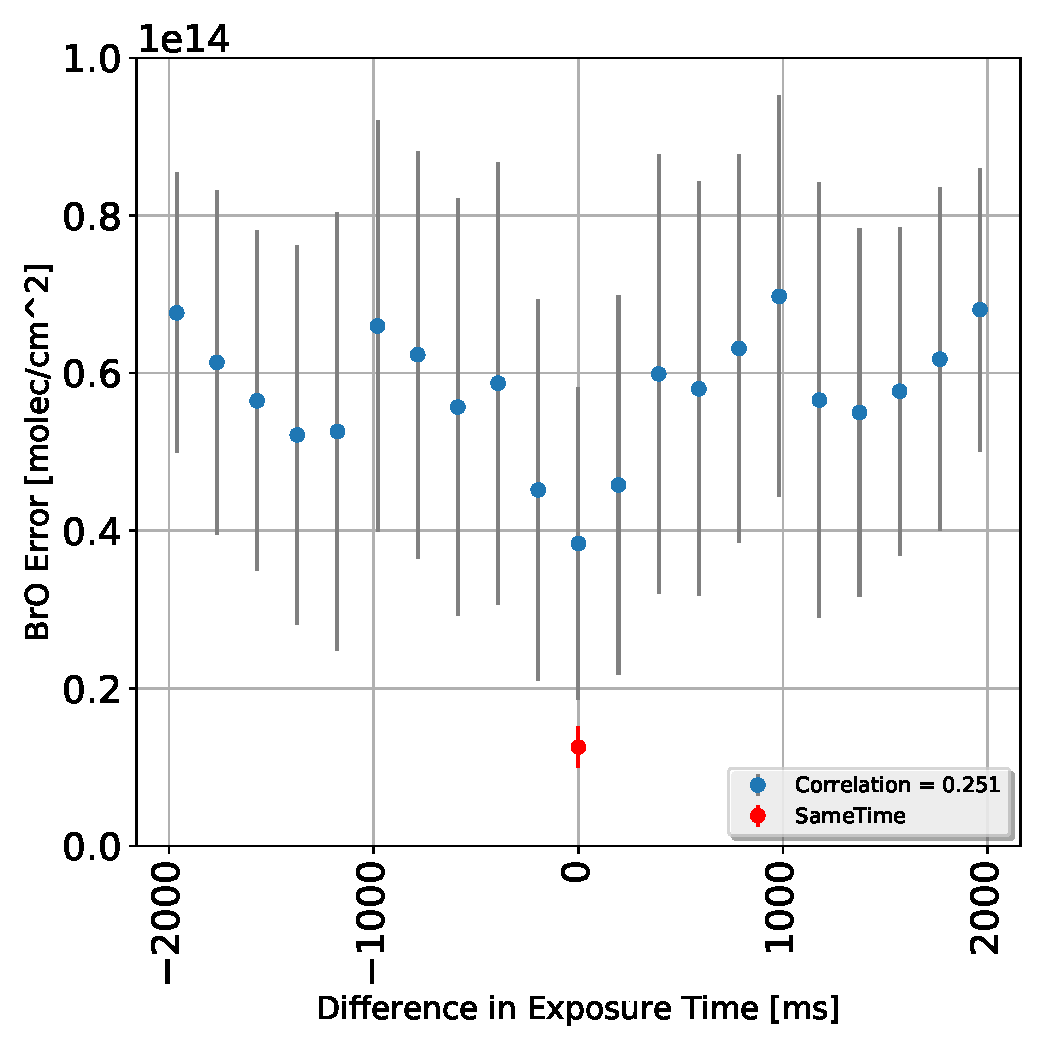
\includegraphics[width=0.3\linewidth]{Bilder/DEpendencoOfBrOErrorOnVariables_absolutedep/I2J8548_0BrOERR_DiffExpTime_Tungu}}
		\centering
		\subfigure[]{\includegraphics[width=0.3\linewidth]{Bilder/DEpendencoOfBrOErrorOnVariables_absolutedep/D2J2200_0BrOERR_DiffExpTime_Nevad}}
		\subfigure[]{\includegraphics[width=0.3\linewidth]{Bilder/DEpendencoOfBrOErrorOnVariables_absolutedep/D2J2201_0BrOERR_DiffExpTime_Nevad}}
		\caption{The \ce{BrO}  measurement error as a function of the difference of exposure time between measuring the reference and the plume are shown. To evaluate the plume spectra all reference spectra with a temporal distance of no longer than two weeks are used. A increase of the \ce{BrO} error with the distance in exposure time is observably.}
		\label{fig:diffexptime}
	\end{figure}
	The Exposure Time is a degree of sky lightness. The  exposure time is the length of time the sensor of the NOVAC instrument is exposed to light. In one scan the exposure time is set constant to the exposure time of the first scan, the pre reference. The amount of light that reaches the film or image sensor is proportional to the exposure time. The exposure time is adjusted in the way that the maximum intensity does not overly the capacity of the sensor.\\
	We can observe an small dependency of the \ce{BrO} error on the Exposure time at Tungurahua and Nevado Del Ruiz as it is shown in \Cref{fig:diffexptime}
	\begin{itemize}
		\item The \ce{BrO}  error as a function of the difference in Exposure Time is also symmetric around zero for all observed instruments, thus the absolute difference in the Exposure Time is sufficient for the evaluating.
		\item The instruments at Tungurahua does not show significantly dependence on the Exposure Time, even though there is always a minimum of the \ce{BrO} error at a difference of the Exposure Time of 0ms.
		\item Nevado Del Ruiz shows a stronger correlation between the \ce{BrO}  error and the Exposure Time.
	\end{itemize}
	\begin{table}[h]
		\begin{tabular}{|p{2cm}|p{2cm}|p{2cm}|p{2cm}|p{2cm}|p{2cm}|}
			%	\toprule
			Instrument	&D2J2140\_0&I2J8546\_0& I2J8548\_0&D2J2200\_0&D2J2201\_0\\
			\toprule
			Slope& 5.54e+9&1.54e+10 &3.04e+10&1.72e+11&9.37e+10\\
			\midrule
			Correlation&0.067
			&0.121&
			0.251&
			0.452&
			0.434\\
			\midrule
			Zero point&4.63e+13&3.58e+13& 3.87e+13& 6.88e+13& 4.68e+13\\
						\midrule
			$\Delta T_{2}$&8357&662&1273&95&499\\
			\bottomrule
		\end{tabular}
		\label{tab:exptimecalc}
	\end{table}

	\begin{itemize}
		\item The \ce{BrO} error increases with the exposure time differences as\\
		\begin{align*}
		\rightarrow&  BrO_{Error} = f(ext. P)+ 1.92\cdot10^{12}\cdot\frac{\Delta ET}{10^{-2}s} + \mathcal{O}\left(\right) & Tungurahua\\
		\rightarrow&  BrO_{Error} = f(ext. P)+ 1.0\cdot10^{13}\cdot\frac{\Delta T}{10^{-2}s} + \mathcal{O}\left(\right) & Nevado Del Ruiz\\
		\end{align*}
	\end{itemize}
	\begin{table}
	\begin{tabular}{|p{2cm}|p{2cm}|p{2cm}|p{2cm}|p{2cm}|p{2cm}|}
		%	\toprule
		Instrument	&D2J2140\_0&I2J8546\_0& I2J8548\_0&D2J2200\_0&D2J2201\_0\\
		\toprule
		Mean&
		81.67$\equiv$ 96,5\%		&162.79$\equiv$ 99,4\%		&212.78$\equiv$ 98,0\%		&283.99$\equiv$ 100,0\%		&225.59$\equiv$ 100,0\% \\
		\midrule
		Std&
		35.30 $\equiv$	98,6\%&		30.07 $\equiv$	100,6\%&
		64.47 $\equiv$	99,5\% &		69.5 $\equiv$	100,0\% &
		41.2$\equiv$	100,0\% \\
		\midrule
		Min  &
		8 $\equiv$	100,0\%\%&113$\equiv$	100,0
		&95 $\equiv$	97,9\%
		&64$\equiv$	100,0\%
		&63$\equiv$	100,0\%\\
		\midrule
		Max&
		167$\equiv$	98,8\% &
		214 $\equiv$	100,0\% &
		395 $\equiv$	99,0\% &
		433 $\equiv$	100,0\%  &
		297 $\equiv$	100,0\% \\
		\bottomrule
	\end{tabular}
	\caption{Amount of Possible references while restricting the difference in Exposure Time  between plume and reference to differences below 632.25ms}
	\label{tab:etrest}
\end{table}	







	\begin{table}
\begin{tabular}{|p{2cm}|p{2cm}|p{2cm}|p{2cm}|p{2cm}|p{2cm}|}
	%	\toprule
	Instrument	&D2J2140\_0&I2J8546\_0& I2J8548\_0&D2J2200\_0&D2J2201\_0\\
	\toprule
	Mean&
	36.0$\equiv$ 42,6\%&	112.9$\equiv$ 69,0\%&
	148.88$\equiv$ 68,6\%&	217.0$\equiv$ 76,4\%&	140.38$\equiv$ 62,2\%\\
	\midrule
	Std&
	22.35 $\equiv$	62,4\%&
	50.6 $\equiv$	169,2\% &
	75.9 $\equiv$	117,1\%&
	82.07 $\equiv$	118,1\% &
	71.0 $\equiv$	172,3\% \\
	\midrule
	Min&
	1 $\equiv$	    12,5\%  &
	8$\equiv$	7,1\%  &
	12 $\equiv$	12,4\%  &
	3$\equiv$	4,7\%   &
	6$\equiv$	9,5\%  \\
	\midrule
	Max
	&127$\equiv$	75,1\%
	&212$\equiv$	99,1\%
	&382$\equiv$	95,7\%
	&398 $\equiv$	91,9\%
	&283$\equiv$	95,3\%\\
	\bottomrule
\end{tabular}
\caption{Amount of Possible references while restricting the difference in colorindex  between plume and reference to differences above 0.2553. maximal Time difference is 3.358$^{\circ}C$,maximal daytime diff is 4.75h without Exposure Time  between plume and reference to differences below 632.25ms}
\end{table}	

\Cref{tab:exptimecalc} shows the slope, correlation, zero point and the $\Delta ET_{2}$s: th differences in Exposure time where the BrO error increases by a factor of two compared to the difference of exposure time of zero.
Restrictions of the exposure Time to the mean of the $\Delta ET_{2}$s of all instruments which is 632.25 ms leads to an average decrease compared to \cref{Tab:refstime} of data of \textcolor{red}{ hier den mittelwert}. The results for each instrument can be found in \cref{tab:etrest}.


	\subsection*{Dependency of external parameters on each other}
	In all those discussions on the impact of the external parameter on the retrieved \ce{BrO}  error the  dependency of the external parameter on each other where neglected. It is plausible that the temperature correlates with the cloudiness or the lightness due to sunlight. Therefore the correlation of the Exposure Time with the \ce{BrO}  error could be a result of the correlation of the Temperature with the \ce{BrO}  error. \Cref{fig:difference-in-exposure-time-msdifference-in-temperature-ctungu} shows an example of the dependency of external parameters on each other. The Difference in Temperature as a function of the Difference in Exposure Time. The \ce{BrO}  error is color-coded. \\
	All correlations between the external parameters are shown in \Cref{fig:varcorrelationmatrix}. \Cref{fig:varcorrelationmatrix} show discrete correlation values from 0.3 to 1. Correlations below 0.3 are ignored. Small plus and minus signs indicate whether the correlation is negative ore positive. 
	The difference in temperature correlates with the difference in daytime (Correlation of $\approx$ 0.5) with the difference in Exposure Time (Correlation of $\approx$ 0.4). The difference in temperature also slightly correlates with the difference in Colorindex (Correlation of $\approx$ 0.3) and the temporal difference (Correlation of $\approx$ 0.3) probably due to long term changes in Temperature. Furthermore the difference in Exposure Time correlates with the daytime and the colorindex (Correlation of $\approx$ 0.4).\\
	\begin{figure}
		\centering
	%	\includegraphics[width=0.7\linewidth]{"../Ausarbeitung/Uebersicht/Bilder/Difference in Exposure Time [ms]_Difference in Temperature [C]_Tungu"}
		\caption{A example of the dependency of external parameters on each other. The difference in Temperature as a function of the Exposure Time. Data from Tungurahua}
		\label{fig:difference-in-exposure-time-msdifference-in-temperature-ctungu}
	\end{figure}
	\begin{figure}
		\centering
		\includegraphics[width=1\linewidth]{Bilder/varCorrelation_matrix}
		\caption{Correlation matrix of the external parameters. The correlation is discrete colour coded. Positive correlation is labeled with a plus whereas negative correlation is labeled with a minus.}
		\label{fig:varcorrelationmatrix}
	\end{figure}
%
		\textbf{Difference of Temperature on  Difference of Exposure Time}
		\begin{equation}
		\Delta T =  -26.32\cdot \Delta ExpTime + 2\cdot 10^{-15}
		\end{equation}
		
		\textbf{Difference of Temperature on  Difference of colorindex}
		\begin{equation}
		\Delta T = 0.0022\cdot \Delta ColIdX +2\cdot 10^{-19}
		\end{equation}
		
				\textbf{Difference of Temperature on  Difference of Day time}
		\begin{equation}
		\Delta T =0.262\cdot \Delta daytime -4\cdot 10^{-17}
		\end{equation}
		
		\textbf{Difference of Temperature on  Difference of Elevation angle}
		\begin{equation}
		\Delta T =1.08\cdot \Delta Elev Angle -1\cdot 10^{-16}
		\end{equation}

		\textbf{Difference of Exposure on  Difference of  Col Idx}
		\begin{equation}
		\Delta Exposure  =-6.22\cdot 10^{-5} \Delta Col Idx  +1\cdot 10^{-18}
		\end{equation}
		
		\textbf{Difference of  Exposure on  Difference of Day time}
		\begin{equation}
		\Delta Exposure  =-0.004\cdot \Delta daytime -1\cdot 10^{-17}
		\end{equation}
		
		\textbf{Difference of  Exposure  on  Difference ofElevation angle}
		\begin{equation}
		\Delta Exposure  =-0.047\cdot \Delta  ElevAngle +3\cdot 10^{-16}
		\end{equation}


		\textbf{Difference of  Colorindex  on  Difference of Day time}
		\begin{equation}
		\Delta ColIdX  =4.51\cdot \Delta daytime-1.2\cdot 10^{-15}
		\end{equation}
		
		\textbf{Difference of  Colorindex  on  Difference of Elevation angle}
		\begin{equation}
		\Delta ColIdX  =-52\cdot \Delta ElevAngle+ 1.45\cdot 10^{-14}
		\end{equation}
		
		\textbf{Difference of  Colorindex  on  Difference of Elevation angle}
		\begin{equation}
		\Delta ColIdX  =3.5\cdot \Delta ElevAngle-6\cdot 10^{-16}
		\end{equation}
	To eliminate the correlation between the external parameters the \ce{BrO}  error dependency on one external parameter where calculated by keeping the differences in the other external parameters constant. The results can be seen in \Cref{fig:DiffExpTime} ( Tungurahua) and \Cref{fig:DiffExpTimeNevad} (Nevado Del Ruiz). When comparing the correlations of the data from \Cref{fig:DiffExpTime} and \Cref{fig:DiffExpTimeNevad}  to the correlations of 
	\Cref{fig:difftemp} to \Cref{fig:diffexptime} a large reduction of the correlation is obvious. Only the difference in Temperature still shows a significant correlation to the \ce{BrO}  error. However the minimal \ce{BrO}  error coincidence in almost all cases with a difference in external parameters of zero. An dependency of the \ce{BrO}  error on the external parameter can still be seen even tough the correlation is very small. And the variability (visualized as the length of the grey bars) increases with increasing difference in external parameters for almost all cases.\\	
	Excluding of the external parameters due to the rather low correlation lead to a worse quality of the results, since the effects of the single parameter ad up to an 
	not negligible amount. Although the added impact of all external parameter except for the temperature are less important than the temperature.
	\begin{figure}
			\subfigure{\includegraphics[width=0.3\linewidth]{Bilder/BrOError_onVariables_050218/I2J8546_0DiffTemp_Tungu}}
			\subfigure{\includegraphics[width=0.3\linewidth]{Bilder/BrOError_onVariables_050218/I2J8548_0DiffTemp_Tungu}}
			\subfigure{\includegraphics[width=0.3\linewidth]{Bilder/BrOError_onVariables_050218/D2J2140_0DiffTemp_Tungu}}
		\subfigure{\includegraphics[width=0.3\linewidth]{Bilder/BrOError_onVariables_050218/I2J8546_0DiffColidx_Tungu}}
		\subfigure{\includegraphics[width=0.3\linewidth]{Bilder/BrOError_onVariables_050218/I2J8548_0DiffColidx_Tungu}}
		\subfigure{\includegraphics[width=0.3\linewidth]{Bilder/BrOError_onVariables_050218/D2J2140_0DiffColidx_Tungu}}

		\subfigure{\includegraphics[width=0.3\linewidth]{Bilder/BrOError_onVariables_050218/I2J8546_0DiffDaytime_Tungu}}
		\subfigure{\includegraphics[width=0.3\linewidth]{Bilder/BrOError_onVariables_050218/I2J8548_0DiffDaytime_Tungu}}
		\subfigure{\includegraphics[width=0.3\linewidth]{Bilder/BrOError_onVariables_050218/D2J2140_0DiffDaytime_Tungu}}

		\subfigure[I2J8546\_0]{\includegraphics[width=0.3\linewidth]{Bilder/BrOError_onVariables_050218/I2J8546_0DiffExpTime_Tungu}}
		\subfigure[I2J8548\_0]{\includegraphics[width=0.3\linewidth]{Bilder/BrOError_onVariables_050218/I2J8548_0DiffExpTime_Tungu}}
		\subfigure[D2J2140\_0]{\includegraphics[width=0.3\linewidth]{Bilder/BrOError_onVariables_050218/D2J2140_0DiffExpTime_Tungu}}
		\caption{DiffExpTime at Tungurahua}
		\label{fig:DiffExpTime}
	\end{figure}


		\begin{figure}
			\centering
			\caption{\ce{BrO} error as a function of the external while measering the Plume and the Reference at Nevado del ruiz}
			\subfigure{\includegraphics[width=0.3\linewidth]{Bilder/BrOError_onVariables_050218/D2J2201_0DiffTemp_Nevad}}
			\subfigure{\includegraphics[width=0.3\linewidth]{Bilder/BrOError_onVariables_050218/D2J2200_0_DiffTemp_Nevad}}\\

			\centering
			\subfigure{\includegraphics[width=0.3\linewidth]{Bilder/BrOError_onVariables_050218/D2J2201_0DiffColidx_Nevad.pdf}}
			\subfigure{\includegraphics[width=0.3\linewidth]{Bilder/BrOError_onVariables_050218/D2J2200_0_DiffColidx_Nevad.pdf}}

			\subfigure{\includegraphics[width=0.3\linewidth]{Bilder/BrOError_onVariables_050218/D2J2201_0DiffDaytime_Nevad}}
			\subfigure{\includegraphics[width=0.3\linewidth]{Bilder/BrOError_onVariables_050218/D2J2200_0_DiffDaytime_Nevad}}\\
			\subfigure[D2J2201\_0]{\includegraphics[width=0.3\linewidth]{Bilder/BrOError_onVariables_050218/D2J2201_0DiffExpTime_Nevad}}
			\subfigure[D2J2200\_0]{\includegraphics[width=0.3\linewidth]{Bilder/BrOError_onVariables_050218/D2J2200_0_DiffExpTime_Nevad}}
			\label{fig:DiffExpTimeNevad}
		\end{figure}
	\subsection*{Summary}
	This chapter examine the influence of external on the precision of the BrO evaluation. Herby the following parameter were considered: 
	Temporal Difference, Temperature, Daytime, Colorindex, Elevation Angle, Exposure Time.  The findings are based on the data of three instruments installed at the Tungurahua volcano and two instruments at the Nevado Del Ruiz volcano. The maximal temporal difference between measuring the plume and the reference was set two 14 days to prevent large uncertainties in the BrO evaluation. Due to the mechanical influence on the wavelength to pixel mapping the temperature has at all analysed instruments the most significant impact on the BrO evaluation of all  considered external parameters. The Elevation Angle does not seem to influence the evaluation for all examined instruments thus the elevation is excluded from the evaluation. The influence of the other external parameter change at every instrument. So a relatively strong impact of the exposure time can be seen at the D2J2201\_0 instrument at Nevado Del Ruiz, while the exposure time does not seem to significantly influence the evaluation of the data from the  I2J8548\_0 at Tungurahua. A large part of the impact of the external parameters results from the dependence on the temperature. 

	\section{\ce{BrO}  dependence on external parameters}
	The external parameters not only influence the fit quality but also the evaluation of the gas amount. A high different in certain external parameter could distort the calculated \ce{BrO}  column density. \Cref{fig:d2j2140060218difftemperature-cbro} shows the evaluation of one Plume with respect to different references. The temporal difference between the references and the plume do not exceed two weeks. In theory we expect that the choice of  the reference should not make a difference, therefore all BrO column densities resulting from the evaluation should be equivalent. But we can see a high variation if choosing different references. The variability of the BrO column density depends as well on the external parameters, when looking at the temperature dependency a mean decrease of th BrO column density with the temperature can be seen. \Cref{fig:d2j2140060218difftemperature-cbro} is a result of an exemplary evaluation of one plume. An examination of all several plumes evaluated by different references is shown in \Cref{fig:alldatacorrwithbrodaytime-plumebro}. Here are equivalent plots shown as for the BrO error (see for example \cref{fig:difftemp}). \Cref{fig:onerefd2j2140060218difftemperature-cbro} shows the exemplary evaluation of different plumes by on reference. Here we assume different column densities, but this variability should be independent of the difference in the external parameters. But \Cref{fig:onerefd2j2140060218difftemperature-cbro} shows a clear dependence on the Temperature. The correlation for this example is -0.76, thus it can be concluded, that here is also an significant dependence. 
	Examination of the Daytime 
	\begin{figure}
		\subfigure[]{
		\includegraphics[width=0.5\linewidth]{"Bilder/OnePlumeMoreRefs_plumedate_081203_1646/D2J2140_0_6_02_18_DiffTemperature [C]_BrO"}}
		\subfigure[]{\includegraphics[width=0.5\linewidth]{"Bilder/OnePlumeMoreRefs_plumedate_081203_1646/D2J2140_0_plumeat12Temperature [C]_BrO_TemporalDiff"}}	
		\caption{One Plume is evaluated by using different references. The plume was recorded at Tungurahua volcano with the D2J2140\_0 instrument. recording time was the 081203 at 1646 o clock. The y axis show the \ce{BrO}  column density differene between the NOVAC method and contamination based Method. (a) The difference in \ce{BrO}  is plotted as a function of the temperature difference between the plume and the references. Every data point indicates one reference. (b) The difference in \ce{BrO}  is plotted as a function of the temporal difference between the one plume and the different references}
		\label{fig:d2j2140060218difftemperature-cbro}		
	\end{figure}
	\begin{figure}
		\subfigure[]{
		\includegraphics[width=0.5\linewidth]{"Bilder/OneRefMorePlumes_refdate_081115_1337/D2J2140_0_onerefTemperature [C]_BrO_TemporalDiff"}}
		\subfigure[]{
		\includegraphics[width=0.5\linewidth]{"Bilder/OneRefMorePlumes_refdate_081115_1337/onerefD2J2140_0_6_02_18_DiffTemperature [C]_BrO"}}
		\caption{One Reference is used to evaluated different Plume spectra. The reference was recorded at Tungurahua volcano with the D2J2140\_0 instrument. recording time was the 081115 at 1337 o clock. The y axis show the \ce{BrO}  column density. (a) The \ce{BrO}  is plotted as a function of the temporal difference between the one reference and the plumes  (b) The \ce{BrO}  is plotted as a function of the temperature difference between the plume and the references. Every data point stands for another plume evaluated with the same reference.}
		\label{fig:onerefd2j2140060218difftemperature-cbro}
	\end{figure}
	\begin{figure}
		\includegraphics[width=0.7\linewidth]{"Bilder/OneRefMorePlumes_refdate_081115_1337/onerefD2J2140_0_6_02_18_DiffDaytime (Plume)_BrO"}
		\caption{The difference of BrO when performing the evaluation with The NOVAC Method minus the contamination based method as a function of the Daytime when measuring the plume. The recording time of the reference was 081115 at 1337 o clock}
		\end{figure}
	\begin{figure}
		\subfigure[]{
		\includegraphics[width=0.5\linewidth]{"Bilder/BrODependencies/AllDataCorrWithBrOElevation Angle [deg]_BrO"}
		}
		\subfigure[]{
		\includegraphics[width=0.5\linewidth]{"Bilder/BrODependencies/AllDataCorrWithBrOExposure Time [ms]_BrO"}
		}
		\subfigure[]{
		\includegraphics[width=0.5\linewidth]{"Bilder/BrODependencies/AllDataCorrWithBrOTemperature [C]_BrO"}
		}
		\subfigure[]{
		\includegraphics[width=0.5\linewidth]{Bilder/BrODependencies/AllDataCorrWithBrOColorindex_BrO}
		}
		\subfigure[]{
		\includegraphics[width=0.5\linewidth]{"Bilder/BrODependencies/AllDataCorrWithBrODaytime (Plume)_BrO"}}
		\caption{The Dependence of the BrO evaluation on external parameter is shown. }
		\label{fig:alldatacorrwithbrodaytime-plumebro}
	\end{figure}
	
	
	%--------------------------------------------------------------------------------------------------------------
	\chapter{Contamination based method}
	Based on the findings about the influence of external parameters on the \ce{BrO} error we developed an algorithm which is able to pick an appropriate volcanic-trace-gas free reference.\\ 
	The first step is, to evaluate every reference with solar atlas spectrum, to check for contamination.	A Spectrum is treated as contaminated if the \ce{SO2} column density of the reference (evaluated with a solar atlas spectrum) is larger as 2$\cdot 10^{17}\frac{molec}{cm^2}$.\\
	\\
	If the reference is contaminated:
	\begin{figure}
\centering
\includegraphics[width=0.7\linewidth]{Bilder/Cont}
\caption{}
\label{fig:Cont}
\end{figure}

	\begin{itemize}
		\item We have a list of possible references where all references are not contaminated and the temporal distance to the plume date is no longer than 14 days.
		\item we calculate of all possible references the differences in the external parameters
		\item We use the analysis of external parameters described above to estimate the \ce{BrO} error of all references
		\item We choose the reference with the smallest estimated \ce{BrO} error as new reference
		\item We evaluate the plume spectra with the new reference.
	\end{itemize}

	%
	The assumption is, that the \ce{BrO} error $\epsilon_{BrO}$ can be described as the sum of $\epsilon_{0}$ and the deviation of $\epsilon_{BrO}$ with respect to all external parameters. $\epsilon_{0}$ is the \ce{BrO} error when evalute the plume spectrum with the "same-time-reference", it is determined due to the accurateness of the NOVAC-instruments.
	\begin{align}
		\epsilon_{BrO} &=  \epsilon_{0}+\frac{d\epsilon}{dt}+\frac{d\epsilon}{d ^{\circ}}+\frac{d\epsilon}{dT}+\frac{d\epsilon}{ddt} +\frac{d\epsilon}{dc} + \mathcal{O}\left(OE\right) \\
		\rightarrow \Delta \epsilon_{BrO} &= \epsilon_{BrO} - \epsilon_{0} =\frac{d\epsilon}{dt}+\underbrace{\frac{d\epsilon}{d ^{\circ}}}_{=0}+\frac{d\epsilon}{dT}+\frac{d\epsilon}{ddt} +\frac{d\epsilon}{dc} + \mathcal{O}\left(OP\right) 
		\label{calc:err}
	\end{align}
	With $\epsilon_{BrO}$ describes the \ce{BrO} error, t: time between plumetime and referencetime, T, temperaure; dt: daytime, c: colorindex, OP: other excluded external parameters\\
	The task occurring at this stage is to find the best representation for the deviations. An then find the reference which minimize $\Delta \epsilon_{BrO} $\\
	%
	\\
	%
	The easiest way is to just calculate the \ce{BrO} error of all possible references for every plume. Using this method we would be able to just choose the reference where the \ce{BrO} error is minimal. But this takes to much time since the evaluation would be proportional to the number of possible references because the evaluation need to be done for every plume-reference pair. Doing the evaluation for every plume-reference pair would make it impossible to do the evaluation in real, or near real time.\\
	%
	But we use this optimal evaluation to rate our model and compare them among each other. The optimal evaluation always choose the reference with the smallest absolute error. We don't use the relative error due to his vulnerability. Using the relative error could lead to a less preciseness.\\
	%
	\\
	Hier ein Bild, das eine Plume gegen viele referencen auswertet und hier die Abweichungen zeigt\\
	\\
	%
	The results of the algorithm which chooses the reference automatically are described relative to an optimal evaluation. If the relative error is larger than 5 we don't use the data.\\
	\\
	We tried several methods for choosing the best reference based on the analysis of external parameters. Fitting the data with a first order polynomial brought the best results.
	
	
	\section{Fit data}
	The following chapter analyses the possibility of fitting the data by a first order polynom. \Cref{fig:difftemp}-\Cref{fig:diffexptime} show the \ce{BrO}  error as a function of external parameters. Hereby are the curves symetric around zero differences in the respective external parameter. Therefore it is not necessary to distinguish between positive or negative deviations from the equal surrounding conditions. Thus the absolute differences can be taken.\\
	\\
	%
	A linear approximation of the \ce{BrO}  error as function of the considered external parameter leads to a variation of  \Cref{calc:err} :
	With linear differentiations of the \ce{BrO}  error with respect to the respective external parameters \Cref{calc:err} can be written as:	
	\begin{equation}
		\Delta \epsilon_{BrO} = a_{t}\cdot\Delta t+a_{ET}\cdot\Delta ET+a_{T}\cdot\Delta T+a_{dt}\cdot\Delta dt +a_{c}\cdot\Delta c + \mathcal{O}\left(OP\right)
		\label{calc:delterr}
	\end{equation}
	%
	To determine the coefficients $a_{x}$ (\Cref{calc:delterr}) the data as from \Cref{fig:difftemp}-\ref{fig:diffexptime} where used.  The fitting was done with an ordinary least square linear regression. In particular we used the python function Linear Regression from the library sklearn \citep{SKlearn}. \\
	
	As can be seen in \Cref{Chap:BROErr} the impact of the different external parameters change for every instrument depending on the location and the instrument themself. 
	Whereas the \ce{BrO}  error not show any dependence on some external parameter at some instrument the error has very strong dependence on the same external parameter at another instrument. An example is the correlation between \ce{BrO}  error of 0.6 at D2J2201\_0 (Nevado Del Ruiz) and a correlation of 0.16 at I2J8546\_0 at the Tungurahua volcano.
	To get a more stable algorithm less external parameter are preferable. Thus we need to distinguish between the stability of the fit, which favours less external parameters and quality of the fit, which favours more external parameters. 
	A preferable solution is, to find a solution which is valid for all instruments at the same time to save calculation time. 
	One possibility is to use all external parameter where the correlation is above a certain number, since we want to get a selection valid for all instruments there are two possibilities: The first one is we decide by using the mean correlation of all instruments, the second option is to use the highest correlation
	
	\begin{table}[h]
		\begin{tabular}{|p{4cm}|p{3cm}|p{3cm}|}
			&  Mean -Correlation&  Highest   -Correlation\\
			\toprule
			Temporal Difference&0.798&	0.92\\
			\midrule
			Temperature &0.798&	0.92\\
			\midrule
			Colorindex &0.3108&	0.409\\
			\midrule
			Exposure Time &0.265&	0.452\\
			\midrule
			Elevation Angle &0.02&	0.067\\
			\midrule
			Daytime &0.395&	0.631\\
			\bottomrule
		\end{tabular}
	\end{table}
	\begin{figure}
		\subfigure[Nevado Del Ruiz]{
			\includegraphics[width=0.5\linewidth]{"Bilder/WelcheEP/Nevado Del Ruiz"}}
		\subfigure[Tungurahua]{
			\includegraphics[width=0.5\linewidth]{Bilder/WelcheEP/Tungurahua}}
		\caption{}
		\label{fig:WelcheEP}
	\end{figure}
	To answer this question quantitatively for the fitting routine we evaluated data of Tungurahua and Nevado Del Ruiz with different combinations of the external parameter described in \Cref{Chap:BROErr}. Since we could not observe any correlation between the \ce{BrO} error and the Elevation angle the external parameter elvation angle was neglected in this analysis. To rate the results for the single instruments (three at Tungurahua and two at Nevado Del Ruiz) the difference to the "optimal evaluation" (explained in \ref{optimal evaition}) was used. Hereby the factor x, a quantity which describes the distinction between the optimal-Method and the contamination based method serves as indicator:
	\begin{equation}
	X = \frac{1}{n}\sum_{k}^{n} \frac{EContBased_{ k}}{EOpt_{ k}}
	\label{eq:mean}
	\end{equation}
	$n$ is the total amount of contaminated spectra, $EOpt$ is the \ce{BrO}  error, in the optimal-evaluation, $EContBased$ is the \ce{BrO}  error, in the contamination based-evaluation. 
	\Cref{fig:WelcheEP} shows the calculations of the x factor for th e Tungurahua and the Nevado Del Ruiz volcano. The x-axis shows the external parameter used for the factor X. The y-axis shows the added factors x for every instrument at the volcanoes. The x factors were weighted with the percentage amount of data.
	The factors X change from instrument to instrument. The results for every instrument can be seen in the appendix (\Cref{fig:I2J8548}). The factors X range from 1.18 to 1.42. Thus the difference is not that large. 
	If using the median and not the mean as described in \Cref{eq:mean} our method is even better than the "optimal method". (soll das beschrieben werden wenn ja hier)\\
	As in \Cref{fig:WelcheEP} can be seen  for both volcanoes the x factor is minimal for the combination of the following external parameters:\\
	
	\begin{table}[h!]
			\begin{tabular}{cccc}
		$\bullet$ Temperature & $\bullet$ Daytime&  $\bullet$ Exposure Time & $\bullet$ Temporal Difference\\
		\label{tab:importantexternalParam}
		\end{tabular}
	\end{table}
%	

	For the final algorithm this combination of external parameters is used.
	The coefficients $a_{x}$ were calculated for each instrument at Nevado Del Ruiz and Tungurahua. Furthermore the coefficients $a_{x}$ are calculated with the combined data from all instruments installed at one volcano. The results for the Nevado Del Ruiz volcano can be found in \Cref{tab:coefNevad} and for the Tungurahua volcano in \Cref{tab:coefTung}.
	\begin{table}
		\subfigure{
			\begin{tabular}{c|c|c}
				\toprule
				Constant\\
				\toprule
				$a_{T}$\\
				\midrule
				$a_{ET}$\\
				\midrule
				$a_{t}$\\
				\midrule
				$a_{dt}$\\
				\midrule
				$a_{c}$\\
				\bottomrule
		\end{tabular}}
		\subfigure[Data of Nevado Del Riz D2J2201\_0]{
			\begin{tabular}{c|c}
				\toprule
				value & import\\
				\toprule
				 7.34e+12&0.840\\
				\midrule
				1.55e+10&0.045\\
				\midrule
				-2.6e+09& 0.0\\
				\midrule
				1.81e+12&0.091\\
				\midrule
				2.30e+13& 0.031\\
				\bottomrule
		\end{tabular}}
	\subfigure[Data of Nevado Del Riz D2J2200\_0]{
		\begin{tabular}{c|c|c}
			\toprule
			value & import \\
			\toprule
		 	1.16e+13&0.908 \\
			\midrule
			2.81e+10& 0.046\\
			\midrule
			-1.7e+09& 0.0\\
			\midrule
			1.08e+12&0.034\\
			\midrule
			3.59e+13& 0.016\\
			\bottomrule
	\end{tabular}}
	\subfigure[Data of Nevado Del Both Instruments]{
		\begin{tabular}{c|c|c}
			\toprule
			value & import \\
			\toprule
			1.07e+13&0.973 \\
			\midrule
			3.48e+10&  0.070\\
			\midrule
			-9.1e+08& 0.0\\
			\midrule
			 1.52e+11&0.006\\
			\midrule
			 -6.81e+13& -0.047\\
			\bottomrule
	\end{tabular}}
	\caption{(a)Data from Nevado Del Ruiz from the D2J2201\_0 instrument. All external parameter where taken into account. $\epsilon_{0} = =  5.404e+12$
			(b)Data from Nevado Del Ruiz from the D2J2200\_0 instrument. All external parameter where taken into account. $\epsilon_{0} = =  1.105e+13$ (c) Data from Nevado Del Ruiz from both instrument. All external parameter where taken into account. $\epsilon_{0} = 1.260e+13$}
		\label{tab:coefNevad}
	\end{table}	
	\begin{table}
	\subfigure{
		\begin{tabular}{c|c|c}
			\toprule
			Constant\\
			\toprule
			$a_{T}$\\
			\midrule
			$a_{ET}$\\
			\midrule
			$a_{t}$\\
			\midrule
			$a_{dt}$\\
			\midrule
			$a_{c}$\\
			\bottomrule
	\end{tabular}}
	\subfigure[Data of Tungurahua D2J2201\_0]{
		\begin{tabular}{c|c}
			\toprule
			value & import\\
	\end{tabular}}
	\subfigure[Data of Tungurahua D2J2200\_0]{
		\begin{tabular}{c|c|c}
			\toprule
				value & import \\

	\end{tabular}}
	\subfigure[Data of Tungurahua Both Instruments]{
		\begin{tabular}{c|c|c}
			\toprule
			value & import \\
		
	\end{tabular}}
		\caption{(a)Data from Tungurahua  from the instrument. All external parameter where taken into account. $\epsilon_{0} = =  5.404e+12$
			(b)Data from Tungurahua from the  instrument. All external parameter where taken into account. $\epsilon_{0} = =  1.105e+13$ (c) Data from Tungurahua from all instrument. All external parameter where taken into account. $\epsilon_{0} = 1.260e+13$}
		\label{tab:coefTung}
	\end{table}			
	Analyse ob der spass mit den correlations zusammenhaengt
	\section{Other approaches}

	Fitting is not the only possibility of finding the optimal referecne out of the list of all possible references.\\
	Also other possibilities were tried to find the best algorithm. In the following two additionally possibilities are presented. Both are based on the findings in \cref{Chap:BROErr}. 

\subsection{Nearest neighbor approach}


Beside linear regression also the nearest neighbor approach can be utilized to estimate the BrO error for the evaluation with a potential reference spectrum.


The nearest neighbor search describes an optimization problem for a given point $m \in \mathbb{R}^n$ and a set $S \subset \mathbb{R}^n$:

%

\begin{align}
\bar{s}(m) = \min_{s \in S} d(m, s) \label{eq:1nn}
\end{align}

%
Here $d(\cdot, \cdot)$ is a distance function that computes the dissimilarity between the two input arguments. Typical distance metrics are the L1 distance $d_{\text{L1} 	
}(m, s) = ||m - s||^2$ or the L2 (also euclidean) distance function $d_{\text{L2} 
}(m, s) = ||m - s||$. 


In many cases not only one nearest neighbor but a set $M$ of $k$ nearest neighbors is of interest. In this case the optimization problem of Eq. \ref{eq:1nn} must be modified to

%

\begin{align}
\bar{S_k}(m) = \min_{S_k \subset S} \sum_{s \in S_k, m \in M} d(s, m) \label{eq:knn}
\end{align}

%

In many cases the nearest neighbor search is used to estimate a target variable $y_m$ for a feature vector $m \in \mathbb{R}^n$. This method assumes a given set feature vectors $S$ for which the target variables $y_S$ are known. Then the target variable $y_m$ for a given $m$ can be estimated by:

%

\begin{align}
y_m = \frac{1}{k} \sum y_S \label{eq:knn_regression}
\end{align}

%

\subsection*{Advantages of the Nearest Neighbor approach}

\begin{itemize}
	
	\item no pre-assumptions about fitting function 
	
\end{itemize}

%

\subsection*{Disadvantages of the Nearest Neighbor approach}

\begin{itemize}
	\item slower
	\item pre-assumptions about feature importance required  
	\item a little worse results
\end{itemize}

%





%Nachteil:

%* länger dauern

%* etwas schlechter

%* normalisieren von Features


%Vorteil:

%* nicht linear




	\subsection{Iterative approach}
	\begin{itemize}
		\item Description of the iterative Method
	\end{itemize}
	The idea of the iterative method was, that the importance of the individual external parameters are very different, that means if we have the list of possible references, we took all referenes where the temperature difference is minimal, so we get a new, much smaller list of possible referenecs. From this list we choose all references where the next external parameter for example the daytime is minimal and get again a new list. We proceed this way with the following external parameters. We experiment with the sequence of the parameters, to increase the success of the method. The final sequence was:
	\begin{equation*}
	Temperature \bullet ................
	\end{equation*} 
	
	\chapter{Comparison with NOVAC evaluation}
	This chapter shows and discuss the difference of the \ce{BrO}, \ce{SO2}  and \ce{BrO}/\ce{SO2}  ratio data when evaluating with the NOVAC-Method, or with the contamination based method.
	The aim is to discover the systematic differences between the different retrievals and to discuss the reliability of the data.\\
	\\
	To obtain the reference with minimal expected  \ce{BrO}  error the calculation of \Cref{calc:delterr} and the corresponding coefficients from \Cref{tab:coefTung} (Tungurahua) and \Cref{tab:coefNevad} (Nevado Del Ruiz) were used. 
	For the retrieval only "Multi Add" data were used. The maximal temporal difference between measuring the reference and the plume is two weeks.
	%
	We do not distinguish between the individual instruments. \\
	\Cref{fig:diffNovac} shows a comparison of the results of contaminated data for performing the evaluation with the NOVAC-method and the contamination based method. The x axis shows the column density of \ce{BrO}  respectively \ce{SO2}  calculated with NOVAC-method, the y axis shows the column density calculated with the contamination based method. Only data are used where the corresponding \ce{SO2}  column density lies above the plume limit ($SO2\_SCD>7\cdot 10^{17}$). Meaning the column densities evaluated with the contamination based method. The corresponding \ce{SO2}  SCD's evaluated with NOVAC could be below $7\cdot 10^{17}$.
	The plots at the left side (\Cref{fig:diffNovac} (a) \& (c)) show the results from the Tungurahua volcano while the plots at the right side (\Cref{fig:diffNovac} (b) \& (d)) show the results from Nevado Del Ruiz volcano. The black solid line shows a linear fit of the data, the dotted line indicates where the both evaluation are equivalent.\\
	\Cref{fig:diffNovac} (a) respectively (b) show the results for the \ce{BrO}  retrieval:
	\begin{itemize}
		\item The \ce{BrO}  column densities retrieved due to the contamination based method have become larger on average compared to the NOVAC method.
		\item An almost constant offset of 1.2$\cdot 10 ^{13}$ (Tungurahua) and 2.0$\cdot 10 ^{13}$ (Nevado Del Ruiz) can be seen.
		\item  Relatively the \ce{BrO}  column densities increase by xy percent when using the contamination based method.
	\end{itemize}
	%
	\Cref{fig:diffNovac} (c) respectively (d) show the results for the \ce{SO2}  retrieval:
	\begin{itemize}
		\item The \ce{SO2}  column densities retrieved due to the contamination based method have become larger for almost every measurement compared to the NOVAC method.
		\item An almost constant offset of 6.5$\cdot 10 ^{17}$ (Tungurahua) and 7.4$\cdot 10 ^{17}$ (Nevado Del Ruiz) can be seen.
		\item  Relatively the \ce{SO2}  column densities increase by xy percent when using the contamination based method.
	\end{itemize}


	\begin{figure}[h!]	
	\subfigure[Data of Tungurahua]{\includegraphics[width=0.5\textwidth]{Bilder/Tungurahua_Pic/tung_bro_novac_conbased}}
	\subfigure[Data of Nevado Del Riz]{\includegraphics[width=0.5\textwidth]{Bilder/NevadoDelRuiz_Pic/bro_novac_conbased}}
	\subfigure[Data of Tungurahua]{\includegraphics[width=0.5\textwidth]{Bilder/Tungurahua_Pic/tung_so2_novac_conbased}}
	\subfigure[Data of Nevado Del Riz]{\includegraphics[width=0.5\textwidth]{Bilder/NevadoDelRuiz_Pic/so2_novac_conbased}}
	\caption{Comparison of the results of contaminated data for performing the evaluation with the NOVAC-method and the contamination based method. Only data are used where the corresponding \ce{SO2}  column density (retrieved from the contamination based method) lies above the plume limit of $SO2\_SCD>7\cdot 10^{17}$. The black solid line shows a linear fit of the data, the dotted line indicates where the both evaluation are equivalent. (a) Results for the \ce{BrO}  column densities from Tungurahua; (b) Results for the \ce{BrO}  column densities from Nevado Del Ruiz; (c) Results for the \ce{SO2}  column densities from Tungurahua; (d) Results for the \ce{SO2}  column densities from Nevado Del Ruiz}
	\label{fig:diffNovac}
\end{figure}
\begin{figure}[h!]		
	\subfigure[]{\includegraphics[width=0.5\textwidth]{Bilder/Tungurahua_Pic/tung_ratio_novac_conbased}}
	\subfigure[]{\includegraphics[width=0.5\textwidth]{Bilder/NevadoDelRuiz_Pic/ratio_novac_conbased}}
	\subfigure[]{\includegraphics[width=0.5\textwidth]{Bilder/Tungurahua_Pic/tung_ratio_diff_novac_conbased}}
	\subfigure[]{\includegraphics[width=0.5\textwidth]{Bilder/NevadoDelRuiz_Pic/ratio_diff_novac_conbased}}
	\caption{Comparison of the results of contaminated data for performing the evaluation with the NOVAC-method and the contamination based method. Only data are used where the corresponding \ce{SO2}  column density (retrieved from the contamination based method) lies above the plume limit of $SO2\_SCD>7\cdot 10^{17}$. (a)+(b): The black solid line shows a linear fit of the data, the dotted line indicates where the both evaluation are equivalent. (a) Results for the \ce{BrO}  /\ce{SO2}  column densities from Tungurahua; (b) Results for the \ce{BrO}  /\ce{SO2}  column densities from Nevado Del Ruiz. 
	(c) +(d) The column density calculated with NOVAC was substracted from the corresponding column density retrieved with the contamination based method. The black valid line indicates a linear fit of the data, the dotted grey line shows where the difference is zero, that means both evaluations lead to the same ratio. (c) Tungurahua (d) Nevado Del Ruiz}
	\label{fig:diffratio}
\end{figure}
\Cref{fig:diffratio} shows the difference of the ration when performing the evaluation with the NOVAC method or the contamination based method. The results for Tungurahua are visualized at the left side (\Cref{fig:diffratio} (a),(c)) and the results for Nevado Del Ruiz are shown at the right side  (\Cref{fig:diffratio} (b),(d)). \Cref{fig:diffratio} (a) and (b) show the results of the contamination based method plotted against the results of the NOVAC method. \Cref{fig:diffratio} (b) and (c) show the actual difference between both method. The column density calculated with NOVAC was substracted from the corresponding column density retrieved with the contamination based method. The black valid line indicates a linear fit of the data, the dotted grey line shows where the difference is zero, that means both evaluations lead to the same ratio.\\
\begin{itemize}
	\item For low \ce{BrO}/\ce{SO2}  ratios approximately below zero, the ratios calculated with the contamination based method are higher than the ratios retrieved with the NOVAC method. For higher \ce{BrO}/\ce{SO2}  ratios (approximately above zero) the ratios calculated with the NOVAC method are larger.
	\item Since the increase of the \ce{SO2}  data is about xxx percentage points higher this evolution of the Ratio is expectable
	\item The absolute difference between both evaluation methods increases with the increase of the absolute ratio
\end{itemize}

Due to the increase of the \ce{SO2}  column density when performing the evaluation with the contamination based method more \ce{SO2}  SCD lie above the plume limit of $7\cdot10^{17}\quad \frac{molec}{cm^2}$. This leads to an increase of the amount of reliable data.\\ 
In the following we will discuss the results for the Tungurahua volcano and the Nevado Del Ruiz. 



\section{Tungurahua}
 	In total in the time span of 080608 to 090830 6500 multi add spectra were recorded. 
 	When performing the evaluation using the NOVAC-Method 6.7 percent of the \ce{SO2}  coloumn densities are in the plume limit. Thus 6.7 percentage of the data can be used for the examination of the volcanic gas emissions in this timespan.
 	6.0 percentage of these spectra are found as contaminated. If the contaminated spectra would be excluded, only 5.5 percent of the \ce{SO2}  column densities are above the plume limit. A higher amount of spectra which \ce{SO2}  limits can be found in the contaminated data. Here the percentage of data in the plumelimit is: 19.2 .
 	Therefore we contaminated data are 2.86 times more frequently above the detection limit. This lead to the presumption, that the possibility of getting contaminated data increases with the gas amount leaving the volcano.
 	
 	To perform the evaluating of the contaminated data with the contamination based method 41.9 percent of the resulting \ce{SO2}  column densities are in the plume limit. Thus the reliable amount of contaminated data increase by 118.7 percentage while the total amount of data increase by 45.2 percent.\\
 	Due to using trace gas free references instead of contaminated references about 45.2 percent more data are available. \\
 	Due to the very small amount of \ce{BrO}  column densities above the detection limit often the daily mean of the \ce{BrO}/\ce{SO2}  ratios is used. Hereby at least tree to four "multi adds" per day in the plume limit need to be recorded. Thus performing the evaluation of contaminated data with the contamination based method leads to more data, thus some days which had less than  tree to four valid data points could then have four ore more multi adds. 12.5 percent more daily mean data can be retrieved when using the contamination based method. The amount of daily means increases less than the total amount of data, this effect can be explained due to a higher occurence of contamination if the \ce{SO2}  column densities are high, thus more data are retrieved for days with high \ce{SO2}  amount.
	\begin{figure}
		\centering
		\includegraphics[width=0.7\linewidth]{Bilder/tung_so2_novac_sametime}
		\caption{}
		\label{fig:tungso2novacsametime}
	\end{figure}
	


\section{Nevado Del Ruiz}
At Nevado Del Ruiz a larger time span where examined thus there is a higher amount of multi ad Data of: 14005.
For the NOVAC evaluation 12.8 percentage are above the detection limit and 9.9 percentage of the data are contaminated.
77.9 percentage of the contaminated data have a \ce{SO2}  coloumn density above $7\cdot10^{17}\quad \frac{molec}{cm^2}$ Thus we have as well a higher occurence of the data above the plume limit within the contaminated data. 
The reliable amount of contaminated data increase by 95 percentage while the total amount of data increase by xy percent.\\
Due to using trace gas free references instead of contaminated references about 87.6 percent more data are available. \\
In total we get 22.6 percent more daily means in the TimeSpan at Nevado Del Ruiz.\\
\\
\\
These data are visualized in \Cref{fig:barplot}. \Cref{fig:barplot} shows a bar plot. The y axis indicates the percentage amount of the data.  The contaminated data are coloured with yellow, the data without contamination are coloured in blue. Data above the plume limit are further marked with black lines.  The left two bars show the result of the Nevado Del Ruiz volcano. The first bar show the findings resulting from the NOVAC evaluation, the second bar the findings of the contamination based method. At the right side are the results from Tungurahua presented in the same way as for Nevado Del Ruiz.\\
\\
%
\begin{table}
	\subfigure{
	\begin{tabular}{p{5cm}p{2cm}p{4cm}p{4cm}}
		&&Tungurahua&Nevado Del Ruiz\\
		\toprule
		Total Amount of Data&&6500&14005\\
		\midrule
		Total amount of Data above Plume Limit&&6.7\%&12.8\%\\
		\midrule
		Contaminated Data &&0.060&0.099\\
		\bottomrule			
	\end{tabular}}
		\subfigure{		
		\begin{tabular}{|p{2cm}p{2cm}p{1.8cm}|p{1.8cm}}
			\multicolumn{3}{c}{Contaminated data}\\
			\toprule
			&&Tungu rahua&Nevado Del Ruiz\\
			\toprule
			\multirow{2}{*}{\shortstack[l]{Within\\ Plume-limit}}& NOVAC&0.192&0.399\\
			&Cont based&0.419&0.779\\
			\midrule
			 not analysable&0.025&0.078\\
			\bottomrule			
		\end{tabular}
	}
	\subfigure{	
		\begin{tabular}{p{2cm}p{1.8cm}|p{1.8cm}|}
			\multicolumn{3}{c}{Not contaminated data}\\
			\toprule
			&Tungu rahua&Nevado Del Ruiz\\
			\toprule
			{\shortstack[l]{Within\\ Plume-limit}}&0.055&0.088\\

			\bottomrule		
		\end{tabular}}
	\end{table}
\section{BrO/\ce{SO2}  time series}
The final time series of \ce{BrO}/\ce{SO2}  for Tungurahua and Nevado Del Ruiz are shown \Cref{fig:resultsnevadodelruiz-1} (Nevado Del Ruiz) and \Cref{fig:resultstungurahua} (Tungurahua).
	Interpretation of the \ce{BrO}/\ce{SO2} ratio time-series
	\begin{figure}
		\centering
		\includegraphics[width=0.7\linewidth]{Bilder/Results/Results_Tungurahua}
		\caption{}
		\label{fig:resultstungurahua}
	\end{figure}



	\begin{small}	
%Menge an Daten insgesamt: ----------------------------------------------------- 6500 ≙ 1
%Davon: Menge an daten (auch kontaminierten)(NOVAC) über plume limit--------- 434  ≙ 0.067
%Davon: Menge an Daten, die nicht Kontaminiert sind:------------------------- 6109 ≙ 0.940
%Davon im Plume-limit:  ------------------------------------------------ 360  ≙ 0.055
%Davon über dem Detection Limit:---------------------------------------- 59   ≙ 0.009
%Davon sind kontaminiert: ---------------------------------------------------- 391  ≙ 0.060
%Menge an Daten die nicht ausgewertet werden konnten:------------------- 226  ≙ 0.025
%Menge an kontamininierten Daten, mit NOVAC, über plume limit:---------- 75   ≙ 0.192 der kont daten
%Menge an contaminierten Daten (Neue Auswertung) über plume limit------- 164  ≙ 0.419
%
%Dh in den kontaminierten daten sind mit NOVAC ausgewerteten daten 2.873 häufiger über dem plume limit

	Dh in den kontaminierten daten sind mit NOVAC ausgewerteten daten \underline{2.485} häufiger über dem plume limit\\	

	\end{small}
	\section*{Nevado Del Ruiz}
		\begin{figure}
		\centering
		\includegraphics[width=0.7\linewidth]{"Bilder/Results/Results_NevadoDelRuiz (1)"}
		\caption{}
		\label{fig:resultsnevadodelruiz-1}
	\end{figure}
	\begin{small}	
%Menge an Daten insgesamt: ----------------------------------------------------- 14005 ≙ 1
%Davon: Menge an daten (auch kontaminierten)(NOVAC) über plume limit--------- 1793  ≙ 0.128
%Davon: Menge an Daten, die nicht Kontaminiert sind:------------------------- 12613 ≙ 0.901
%Davon im Plume-limit:  ------------------------------------------------ 1238  ≙ 0.088
%Davon über dem Detection Limit:---------------------------------------- 234   ≙ 0.017
%Davon sind kontaminiert: ---------------------------------------------------- 1392  ≙ 0.099
%Menge an Daten die nicht ausgewertet werden konnten:------------------- 306  ≙ 0.078
%Menge an kontamininierten Daten, mit NOVAC, über plume limit:---------- 556   ≙ 0.399 der kont daten
%Menge an contaminierten Daten (Neue Auswertung) über plume limit------- 1085  ≙ 0.779
%
%Dh in den kontaminierten daten sind mit NOVAC ausgewerteten daten 3.120 häufiger über dem plume limit
%
%	Dh in den kontaminierten daten sind mit NOVAC ausgewerteten daten \underline{3.449} häufiger über dem plume limit\\
 	
 \end{small}
	\chapter{Issues of our method}
	The presented method is questionable since we did not consider contamination of the plume due to a lack of information. And we did not consider the different lifetimes of SO2 and BrO. This leads to a faster 
	
	\section{Contamination of the plume}
	\begin{figure}
		\centering
		\includegraphics[width=0.7\linewidth]{Bilder/Contaminationplume}
		\caption{Visualization of the contamination of the plume. An old plume of the day before. Due to a lack of wind the plume sinks down an accumulates above the instrument. The light path trough the old plume is longer when recording the reference spectra (orange).}
		\label{fig:contaminationplume}
	\end{figure}
	 As discussed above it might occur, that, the plume is contaminated as well. This might be the case if the volcanic gas of the volcano is not taken away by the wind, but accumulates at the instrument. If this is the case, using an contamination free reference of another time would lead to an overestimation of the column density of gases.\\
	 The contamination of the plume is visualized in \Cref{fig:contaminationplume}. This is one possible occurence of contamination. As it can be seen gas of the old plume affected the measurement of the reference and the plume. However for this example the influence on the measurement of the reference is much larger since the light path trough the old plume (coloured orange in \Cref{fig:contaminationplume}) is longer for the reference than for the measurement of the volcanic plume. Thus we underestimate the Gas amount if we do not use an gas free reference, but overestimate if we do so.
	 The real gas amount might be between the measured amount with and without using a reference measured at another time.\\
	 The contamination set up could differ from \Cref{fig:contaminationplume}. This would lead to different results. However the reference region is in most of the time at a larger elevation angle than the plume, thus, the assumption that the light pass trough the old plume is on the average longer for the reference, of both reference and plume are contaminated.
	 
	  With the data retrieved by the NOVAC instruments it is very difficult up to impossible to discover whether the plume is contaminated or not. 




	\chapter{Conclusion}
	In this thesis we made investigations on the contamination of the plume 
	We found an significant increase of the SCDs of SO2 and BrO while the conatmination based evaluation leads to a higher increase of the SO2 amount compared to the BrO evaluation. Thus the BrO/SO2 ratio decreases for values above zero.\\
	\cite{geeignete quelle, irgendwo hab ich das schon gehoert} made investigations on the lifetime of SO2 and BrO. The lifetime of SO2 can reach to several weeks, while the decay of BrO proceed in faster times. As a result we should observe a lower contamination of BrO. This could be observed in our results. In theory it could be that due to the smaller lifetimes of BrO contamination only influences the SO2 evaluation, if that is the case, the best option would be to use a high defined solar atlas spectrum as reference for the SO2 evaluation, but an reference recorded with the same instrument at the same time for the BrO evaluation, since BrO could not be retrieved using an high defined 

	
	
	



  \part{Appendix}
  \begin{appendix}
	\begin{figure}
		\subfigure[]{\includegraphics[width=0.45\linewidth]{Bilder/WelcheEP/D2J2140}}
		\subfigure[]{\includegraphics[width=0.45\linewidth]{Bilder/WelcheEP/D2J2200_0}}
		\subfigure[]{\includegraphics[width=0.45\linewidth]{Bilder/WelcheEP/D2J2200_1}}
		\subfigure[]{\includegraphics[width=0.45\linewidth]{Bilder/WelcheEP/D2J2201_0}}
		\subfigure[]{\includegraphics[width=0.45\linewidth]{Bilder/WelcheEP/I2J8546}}
		\subfigure[]{\includegraphics[width=0.45\linewidth]{Bilder/WelcheEP/I2J8548}}
		\caption{}
		\label{fig:I2J8548}
		\end{figure}
	\subsection*{Fuigures to more plumes to one ref}
	\begin{figure}
		\subfigure[]{
		\includegraphics[width=0.5\linewidth]{Bilder/OneRefMorePlumes_refdate_081115_1337/D2J2140_0_onerefColorindex_BrO_TemporalDiff}
			}
		\subfigure[]{
		\includegraphics[width=0.5\linewidth]{"Bilder/OneRefMorePlumes_refdate_081115_1337/D2J2140_0_onerefDaytime (Plume)_BrO_TemporalDiff"}
				}
		\subfigure[]{
		\includegraphics[width=0.5\linewidth]{"Bilder/OneRefMorePlumes_refdate_081115_1337/D2J2140_0_onerefElevation Angle [deg]_BrO_TemporalDiff"}
				}
		\subfigure[]{
		\includegraphics[width=0.5\linewidth]{"Bilder/OneRefMorePlumes_refdate_081115_1337/D2J2140_0_onerefExposure Time [ms]_BrO_TemporalDiff"}
			}\\
		\subfigure[]{
		\includegraphics[width=0.5\linewidth]{Bilder/OneRefMorePlumes_refdate_081115_1337/onerefD2J2140_0_6_02_18_DiffColorindex_BrO}
			}
		\subfigure[]{
		\includegraphics[width=0.5\linewidth]{"Bilder/OneRefMorePlumes_refdate_081115_1337/onerefD2J2140_0_6_02_18_DiffElevation Angle [deg]_BrO"}
			}\\
	
		\subfigure[]{
		\includegraphics[width=0.5\linewidth]{"Bilder/OneRefMorePlumes_refdate_081115_1337/onerefD2J2140_0_6_02_18_DiffExposure Time [ms]_BrO"}
			}
		\caption{}
		\label{fig:donerefd2j2140060218difftemperature-cbro}
	\end{figure}
	
    \chapter{Lists}
    \listoffigures
    \listoftables
    \bibliography{references}{}
    \citestyle{egu}
    \bibliographystyle{plainnat}
    \setlength{\parindent}{0em}

Erkl\"{a}rung:\par
\vspace{3\baselineskip}
Ich versichere, dass ich diese Arbeit selbstst\"{a}ndig verfasst habe und keine
anderen als die angegebenen Quellen und Hilfsmittel benutzt habe.\par
\vspace{5\baselineskip}
Heidelberg, den (Datum)\hspace{3cm}\dotfill

  \end{appendix}
\end{document}




